% Comment R1 - 1 
\begin{bibunit}

\begin{spacing}{1}
\justifying \color{darkdarkgray} \noindent

Thank you very much for your thoughtful and constructive feedback, which has substantially improved the paper. In particular, your comments on the institutional framing of \emph{Plan Cuadrante} were particularly useful: they led us to contact Carabineros de Chile directly and substantially expand Section 2 with new institutional detail. We also found the literature you pointed us to very helpful in sharpening our contribution. Your comments on mechanisms were equally valuable and led us to substantially reframe that discussion. More generally, we have carefully considered all your comments and hope that we adequately addressed your questions and suggestions in the revised manuscript and in the response document below.


\end{spacing}



\begin{refcomment}

\textbf{Institutional setting and framing}: I think the paper needs to explain the setting in more detail. For instance, how policing was organized before the reform and where officers were based? The paper states quadrants were subdivided into seven units with about 3 officers on average, but what were the corresponding figures prior to the reform? Were officers simply reallocated (e.g. centralized and moved from one place to another) or did the reform also entail an increase in the overall level of resources for front-line policing? This is key for understanding what the counterfactual would have been and therefore for interpreting the policy’s effects (see point 2 below).



\label{pt:r1_01}
\end{refcomment}

% Our reply to R1 - 1 
\begin{response}
	%1. What does Plan Cuadrante identify?
%The paper states in various places that permanent geographic assignment and greater local knowledge are the key mechanisms underlying the RF effects of the policy. I think this interpretation is stronger than what the evidence can establish.
%
%Plan Cuadrante appears to have changed several features of frontline policing simultaneously. Assigning officers to smaller quadrants changes not only the officer-area relationships, but also the spatial organization of police presence. Depending on quadrant size, number of officers, and deployment practices, the reform may have effectively changed police density and patrol intensity, as well as response times. Each of these margins could plausibly affect crime, victimization, perceptions of safety, and citizen cooperation. Greater local knowledge is one compelling mechanism within this bundle, but it is not separately observed from these other operational changes.
%
%I therefore think the paper should explicitly acknowledge that the results identify the effect of a broader organizational and deployment reform rather than the effect of local knowledge alone. A more defensible interpretation would be that Plan Cuadrante, combining permanent officer-to-quadrant allocation with an increase in police density, improved public safety and citizens' perceptions of the police. Even holding the total number of officers fixed, reorganizing officers across smaller territorial units may change the intensity and concentration of local police presence.
%
%One potentially useful exercise would be to characterize police density across quadrants, for example in terms of officers per square kilometer (or per capita). The illustrative map in the paper suggests that quadrants vary substantially in geographic size (and the smaller quadrants are the ones with higher baseline crime rates). If the authors observe the number of officers assigned to each quadrant, it would therefore be useful to document the distribution of officers per quadrant, and examine whether treatment effects vary with this measure of effective local police density. Police density may itself be correlated with response times, patrol intensity, and other operational margins, so it would still not isolate a single mechanism. But it would help characterize an important dimension of what the reform changed.



\end{response}

\stepcounter{AnsweredComments}


\begin{refcomment}

 \smallskip
Relatedly, I find the label “geographic specialization” potentially misleading, as it may suggest policing efforts concentrated in specific city areas, which is not how the paper currently reads. In the economics of crime literature, similar interventions are more often described as “hot-spot policing,” in contrast with approaches that aim to maintain constant response times. Can the authors directly compare this reform to these? Alternatively, if the reform went beyond territorial reallocation to include changes in personnel assignments (e.g., shifting away from office to street duties) or shifts in decision-making from central to local levels, this should be explained clearly, since it would ultimately shape the paper’s contribution (see also point 3 below).

\end{refcomment}

% Our reply to R1 - 2 
\begin{response}
	%2. Resource changes
%Figure 4 is most informative in the comparison between the bottom 40 percent of treated municipalities and control municipalities, which experienced similar resource growth. The interpretation should nevertheless be cautious. In particular, not even the bottom group or the control group experience zero resource growth. The exercise therefore does not isolate the effects of the geographic reorganization, absent those of changes in resources. Rather, it shows that the estimated gains are not confined to municipalities experiencing the largest resource expansions.
%
%Relatedly, I think Table B3 is helpful. I would not dismiss these specifications simply because resource changes are themselves induced by treatment. Conditioning on policy-induced resource changes can still be informative about whether the reduced-form effect is concentrated in places experiencing large resource expansions.


%Internal note: No he cambiado el paper para responder a esta pregunta. Seria quitar la footnote y poner en su lugar el texto que se pone mas abajo. El apendice es igual.

Thank you very much for these comments.

On the comparison between municipalities with control-like versus larger resource growth: we agree with your characterization and do not read this exercise as isolating the effect of the geographic reorganization from that of resource changes. Our point is narrower. Finding sizeable effects even among municipalities whose resource growth resembles that of the control group does not mean that resource growth was unimportant---resources may well have been necessary to enable the effective implementation of the deployment reorganization even in that municipalities---but it does indicate that the reorganization itself plays an important role. This qualification is in the updated paper. For example, in the Introduction, we state that ``these patterns indicate that while resource increases helped enable implementation and may explain part of the effects in some municipalities, the beat-policing components of the reform were central drivers of the overall gains.'' In Section \ref{mechanisms}, we similarly state that ``although we cannot fully separate the beat policing component from the resource component of the reform---resources may have been important to enable effective implementation of the program, or may explain part of the effects in some municipalities---the fact that municipalities with resource increases similar to those experienced by control municipalities still display sizeable effects indicates that the effects of \emph{Plan Cuadrante} are not driven entirely by resources.''

Regarding Table B3: thank you for the suggestion; we agree these estimates are informative. This is now discussed directly in the main text of Section \ref{mechanisms}, rather than only in a footnote, in addition to the Online Appendix. 

We included the following text in section 4.4: ``As a further check, we re-estimate the results in Figure 2 controlling directly for police resources. Online Appendix Table \ref{tab:results_controlbyresources} shows that the magnitude of the estimated effects remains similar for most variables, although the statistical significance is reduced in some estimations. This likely reflects a mechanical feature of the \citet{Callaway} estimation procedure: control variables are not incorporated parametrically, but are instead used to construct the comparison group via outcome regression or propensity-score weighting, so the resulting estimation uncertainty propagates to the ATT standard errors. Note, however, that police resources are probably a bad control---i.e., at least part of their variation is a result of the adoption of \emph{Plan Cuadrante}---so these results should be interpreted cautiously.'' 


The Online Appendix (Section \ref{resources_plan_cuadrante}) reads: ``The results of this analysis are reported in Table \ref{tab:results_controlbyresources}. The magnitude of the estimated effects remains similar for most variables, although the statistical significance is reduced in some estimations. This likely reflects a mechanical feature of the \citet{Callaway} estimation procedure: control variables are not incorporated parametrically, but are instead used to construct the comparison group via outcome regression or propensity-score weighting, so the resulting estimation uncertainty propagates to the ATT standard errors. Note, however, that these resource variables are bad controls, as they are affected by the adoption of \emph{Plan Cuadrante}, so these results should be interpreted with caution.''


    
\end{response}
\stepcounter{AnsweredComments}


\begin{refcomment}
\smallskip

\textbf{Policy impacts and increases in police resources}: At present, the paper provides too little detail, leaving the reader unsure about how to interpret results of a reform that changed multiple aspects of policing.

1. The policy seems to have changed for some cities the allocation of resources conditional on total levels, and for some others the aggregate levels too. The authors attempt to address this in Figure 5, however a few points are still unclear. In Panels C and D, the first bar seems to suggest that even the control group experienced increases in the number of officers. Could the authors clarify why this is the case, and how large these increases were relative to baseline levels? In addition, Panel E and F show the effects on crime perceptions and reported crime for municipalities with small versus large increases in police forces. The point estimates differ, and the overlapping confidence intervals may simply reflect low statistical power (given a sample size of N=200/300). Thus, the conclusion that “resource increases alone were not sufficient to improve police effectiveness” seems premature. Perhaps more importantly, this would contrast with much of the existing literature on police strength and crime, and it would be helpful if the authors clarified how they interpret their findings in light of this.

\label{pt:r1_03}
\end{refcomment}

% Our reply to R1 - 3 
\begin{response}
	%Minor point: in Panel D in Table B3, the sample size falls substantially when the officer control is added. Why?


 
\end{response}
\stepcounter{AnsweredComments}

\begin{refcomment}
\smallskip
2. I think Table C2 is a first step in the right direction. However, Equation (5) should include both controls for N of officers and cars, so that it can approximate a police production function as closely as possible. Ideally, one would like to run a specification that includes the policy indicator together with N of officers and cars, but I understand that the policy dummy drops out in a regression at the municipality-year level. A viable option would be to interact treatment dummy with an indicator for municipalities that experienced larger increases in officers or vehicles. Alternatively, a mediation analysis could help quantify the extent to which resource increases account for the total observed effects of the policy. Finally, I am not fully convinced by the statement “lack of statistical association between police resources and the main outcomes” since several coefficients in Table C2 appear significant. This also suggests that resources may play a more substantive role than currently acknowledged.

\label{pt:r1_04}
\end{refcomment}

% Our reply to R1 - 4 
\begin{response}
	%3. Contribution and framing
%I would simplify the framing of the paper's contribution. The findings provide evidence that the organization and territorial deployment of police resources matter for public safety (and for citizens' perceptions, which by itself is a quite novel result), even though the specific mechanisms generating these gains cannot be fully decomposed. I think this is an interesting and important contribution on its own, and it does not require attributing the effects specifically to local knowledge.


Thanks for the suggestion. Following reviewer's recommendation, we have edited key parts of the paper. The updated sentences read as follows:

XX XX 
\end{response}
\stepcounter{AnsweredComments}



\begin{refcomment}
\smallskip

3. The paper should also discuss subsequent adjustments to the policy in 2007, and the potential disruption created by the 2010 earthquake. Both could have affected treatment quality/intensity (or even the different components?) as well as local perceptions, and it is important to explain how these events are handled in the empirical section. For example, is it possible to exclude the affected areas, or to test whether the earthquake generated changes in perceptions that confound the results? At the same time, could the 2007 adjustment and 2010 earthquake be exploited as sources of heterogeneity to shed light on mechanisms if they were different in nature?

\label{pt:r1_05}
\end{refcomment}

% Our reply to R1 - 5 
\begin{response}
	%2.3- The paper should also discuss subsequent adjustments to the policy in 2007, and the potential disruption created by the 2010 earthquake. Both could have affected treatment quality/intensity (or even the different components?) as well as local perceptions, and it is important to explain how these events are handled in the empirical section. For example, is it possible to exclude the affected areas, or to test whether the earthquake generated changes in perceptions that confound the results? At the same time, could the 2007 adjustment and 2010 earthquake be exploited as sources of heterogeneity to shed light on mechanisms if they were different in nature?

In 2007, an evaluation conducted by DIPRES (Chile's Directorate of Budget, an independent government body) recommended the formalization of new specialized roles within each police station, including a Head of Operations Office, a Community Affairs Officer, and officers responsible for drug prevention, domestic violence, and judicial orders \citep{DIPRES2007_largo}. However, these changes were more formal than operational, and were not effectively implemented at scale until the introduction of \emph{Plan Cuadrante 2.0}, outside our study period. The 2014 DIPRES evaluation documents, for example, that while the Community Affairs Officer role was formally created in some municipalities, dedicated personnel and budget were not assigned, and the community integration model (MICC) was only piloted in 4 to 6 police stations in 2012--2013 (none of these stations were in municipalities in our analytical sample) before its financing agreement was discontinued in early 2014 \citep{DIPRES2014,Manual_Carabineros2018}. Similarly, the Operations Office lacked the digitalization, personel, and dedicated resources needed to fulfill its analytical functions until the launch of \emph{Plan Cuadrante 2.0} \citep{DIPRES2014, Manual_Carabineros2018}. Our results therefore capture the effects of the original \emph{Plan Cuadrante}, characterized primarily by the reduction of police catchment areas and the permanent territorial assignment of officers, without contamination from the more substantive operational reforms introduced later.

Regarding the disruption that the 2010 earthquake in Concepcion could have on the implementation of \emph{Plan Cuadrante}: The 2010 earthquake halted the expansion of the program. No new municipalities joined the program in 2010. Moreover, it could potentially confound our estimates on outcomes if it differentially affected treated and control municipalities, either by disrupting police operations and thus reducing treatment intensity, or by independently affecting crime perceptions and security outcomes in ways unrelated to \emph{Plan Cuadrante}. To address this concern, in the revised manuscript we re-estimate our main results excluding municipalities more exposed to the earthquake, defined as those experiencing a Modified Mercalli Intensity greater than 7. This corresponds to 21 municipalities in the ENUSC sample and 158 municipalities in the administrative data sample. The results, reported in Figure \ref{fig:figure02_noEQ}, are nearly identical to the main estimates, suggesting that the 2010 earthquake does not confound our estimates.

We have added the following footnote in Section 4.1 of the updated manuscript:

\begin{adjustwidth}{2em}{0em}
These results are robust to excluding municipalities most affected by the 2010 Maule earthquake, defined as those with a Modified Mercalli Intensity greater than 7; see Figure \ref{fig:figure02_noEQ} in Online Appendix \ref{sec:appendixC} for details.
\end{adjustwidth}

We also add the following subsection, ``Robustness to the 2010 Earthquake,'' to Online Appendix C reporting this exercise in detail:

\begin{adjustwidth}{2em}{0em}
The 2010 Maule earthquake could confound our estimates if it differentially affected treated and control municipalities, either by disrupting police operations and thus reducing treatment intensity, or by independently affecting crime perceptions and security outcomes in ways unrelated to \emph{Plan Cuadrante}. To address this concern, we re-estimate our main results excluding municipalities more exposed to the earthquake, defined as those experiencing a Modified Mercalli Intensity greater than 7. This corresponds to 21 municipalities in the ENUSC sample and 158 municipalities in the administrative data sample. The results, reported in Figure \ref{fig:figure02_noEQ}, are nearly identical to the main estimates, confirming that the 2010 earthquake does not drive our findings.
\end{adjustwidth}

Regarding the suggestion to exploit the earthquake as a source of heterogeneity, we agree this is an interesting analysis that might help shed light on the mechanisms. To assess the heterogeneous effects of \emph{Plan Cuadrante} by exposure to the earthquake, we estimate the effects of the program separately for municipalities more exposed to the earthquake (Modified Mercalli Intensity greater than 7) and municipalities with a Modified Mercalli Intensity of 7 or lower. The results are reported in Figure \ref{fig:heterogeneity_earthquake_mmi}. They show relatively similar effects across the two groups for both victimization and crime perception. The effects on investment in security measures and reported crime appear somehow larger for municipalities less exposed to the earthquake, although they remain statistically significant for the more affected municipalities as well.



\clearpage
\noindent\textbf{Other figure referenced above:}
\vspace{0.5em}

{\renewcommand{\thefigure}{C.11}
%--- Robustness check: 2010 Maule earthquake (Mercalli > 7 excluded)
\begin{figure}[h!]
    \centering
    \caption{Effects of \emph{Plan Cuadrante} excluding Municipalities Affected by the 2010 Earthquake}
    \label{fig:figure02_noEQ}
    \begin{subfigure}{0.495\textwidth}
        \centering
        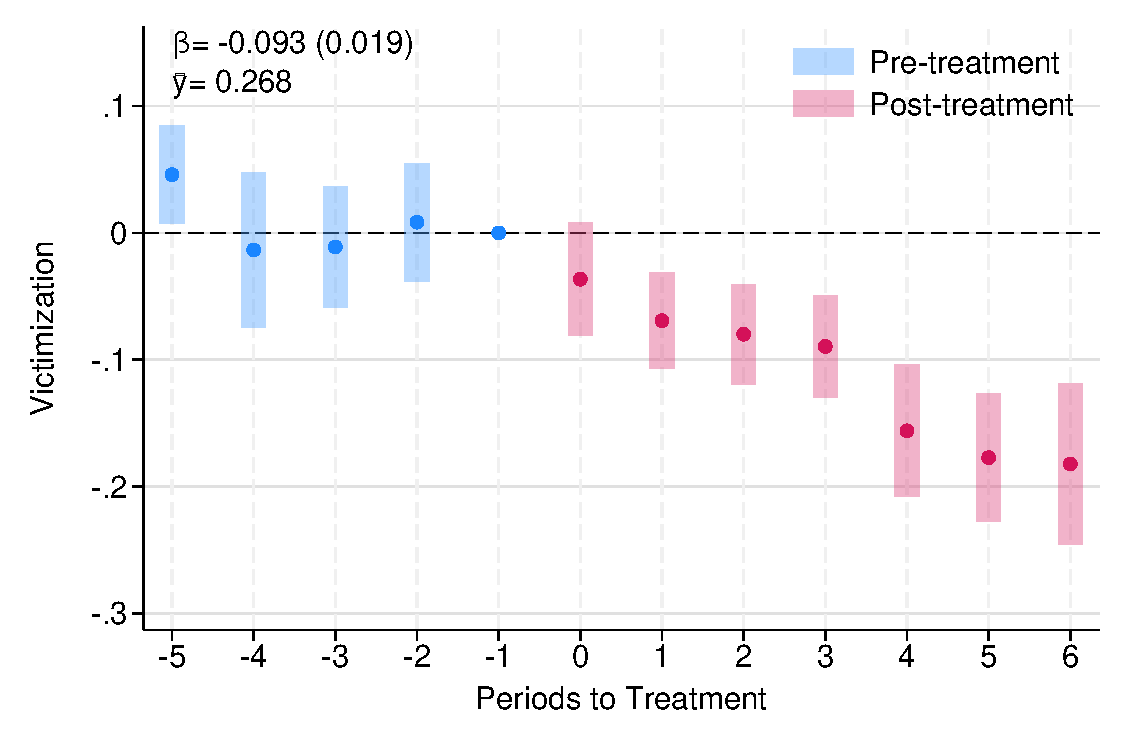
\includegraphics[width=\textwidth]{../manuscript/Graphs/results_victimization_noEQ.pdf}
        \caption{Victimization in last 12 months}
    \end{subfigure}%
    ~
    \begin{subfigure}{0.495\textwidth}
        \centering
        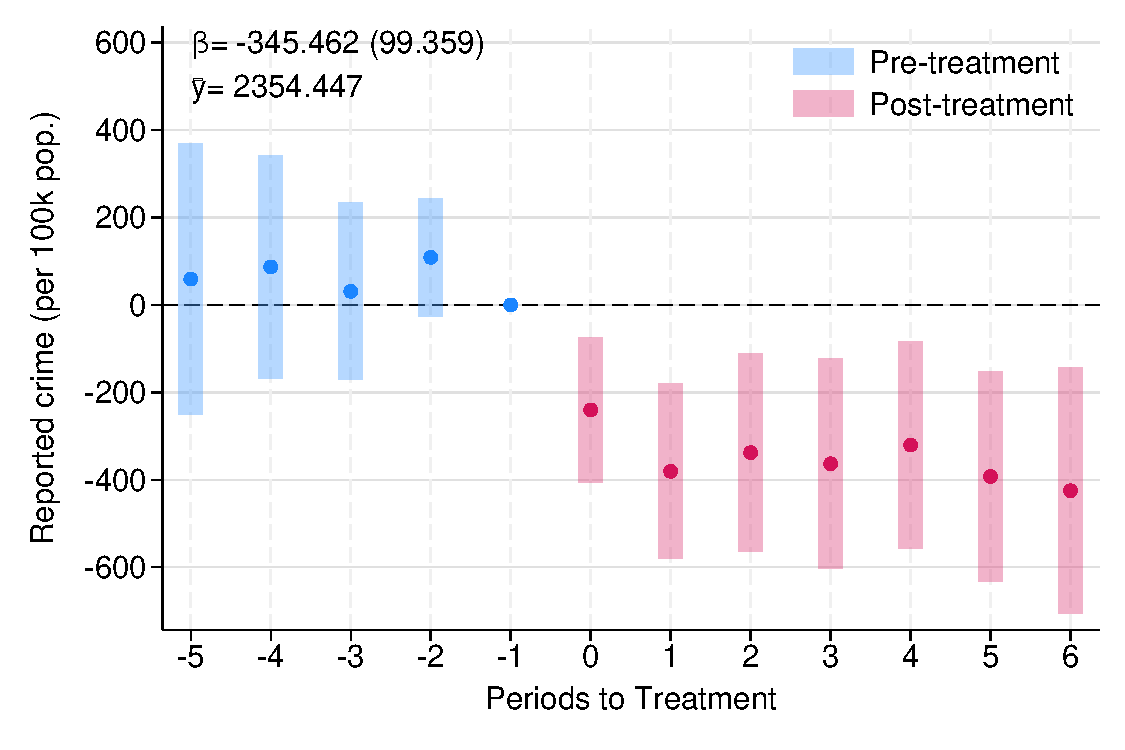
\includegraphics[width=\textwidth]{../manuscript/Graphs/totalreportedcrime_allcomunas_noEQ.pdf}
        \caption{Reported crime per 100k inhabitants}
    \end{subfigure}
    \begin{subfigure}{0.495\textwidth}
        \centering
        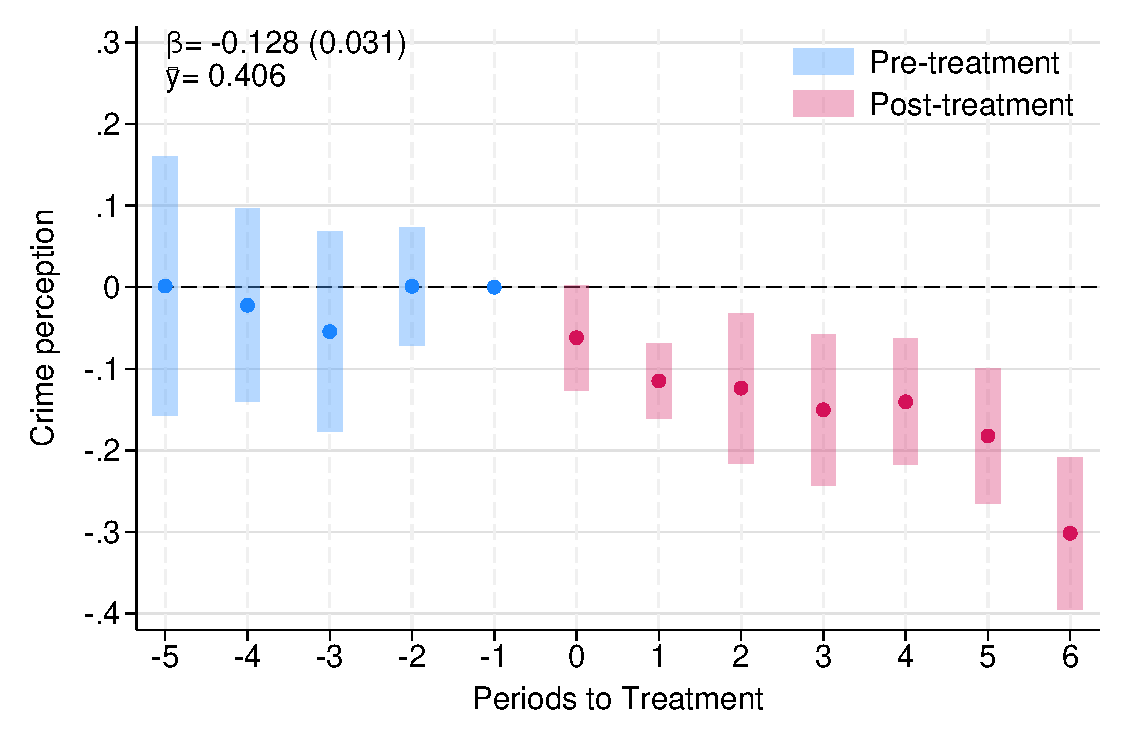
\includegraphics[width=\textwidth]{../manuscript/Graphs/results_perception_noEQ.pdf}
        \caption{Households reporting an increase in crime}
    \end{subfigure}%
    ~
    \begin{subfigure}{0.495\textwidth}
        \centering
        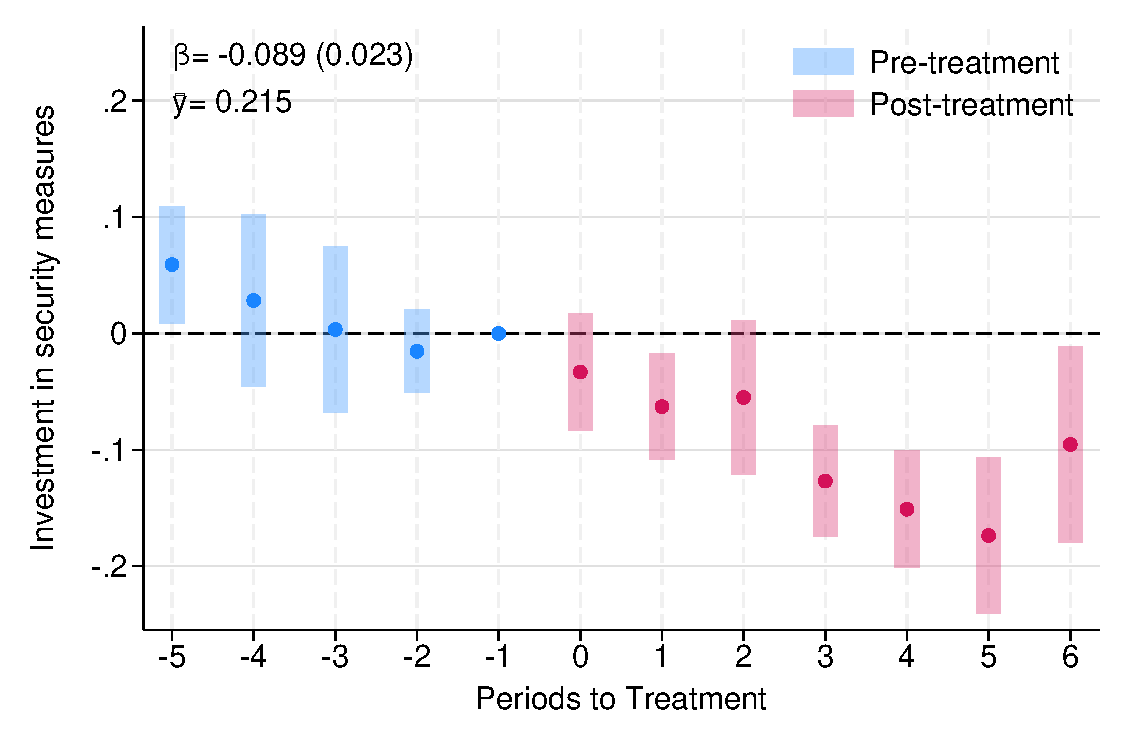
\includegraphics[width=\textwidth]{../manuscript/Graphs/results_hhprotectionmeasures_noEQ.pdf}
        \caption{Households adopting security measures}
    \end{subfigure}
    \\[12pt]
    \begin{minipage}{0.99\textwidth}
    \footnotesize
    Notes: This figure replicates the results of Figure \ref{fig:figure02} after excluding municipalities affected by the 2010 Maule earthquake, defined as those with a Modified Mercalli Intensity (MMI) score strictly greater than 7. The estimation is conducted using the procedure developed in \citet{Callaway} for difference-in-differences with staggered treatment adoption. The dots in the figure represent the estimated coefficients and the bars behind them 95\% confidence intervals. Standard errors are clustered at the municipality level using the wild bootstrapping procedure. The pooled effect and the mean outcome before the introduction of the treatment is also presented in each panel. Panel (a) reports the effect of \emph{Plan Cuadrante} on the probability of household victimization in the last 12 months using the ENUSC survey. Panel (b) reports the effect on the number of crimes reported to the police in the municipality per 100,000 inhabitants using administrative data. Panel (c) reports the effect on the probability of perceiving an increase in crime using the ENUSC survey. Panel (d) reports the effect on the probability of adopting security measures in the last twelve months using the ENUSC survey.
    \end{minipage}
\end{figure}
}


\begin{center}
{\renewcommand{\thefigure}{S1}
%--- Heterogeneity by exposure to the 2010 Maule earthquake (MMI > 7), all adopters
\begin{figure}[h!]
    \centering
    \caption{Effects of \emph{Plan Cuadrante} by Exposure to the 2010 Earthquake}
    \label{fig:heterogeneity_earthquake_mmi}
    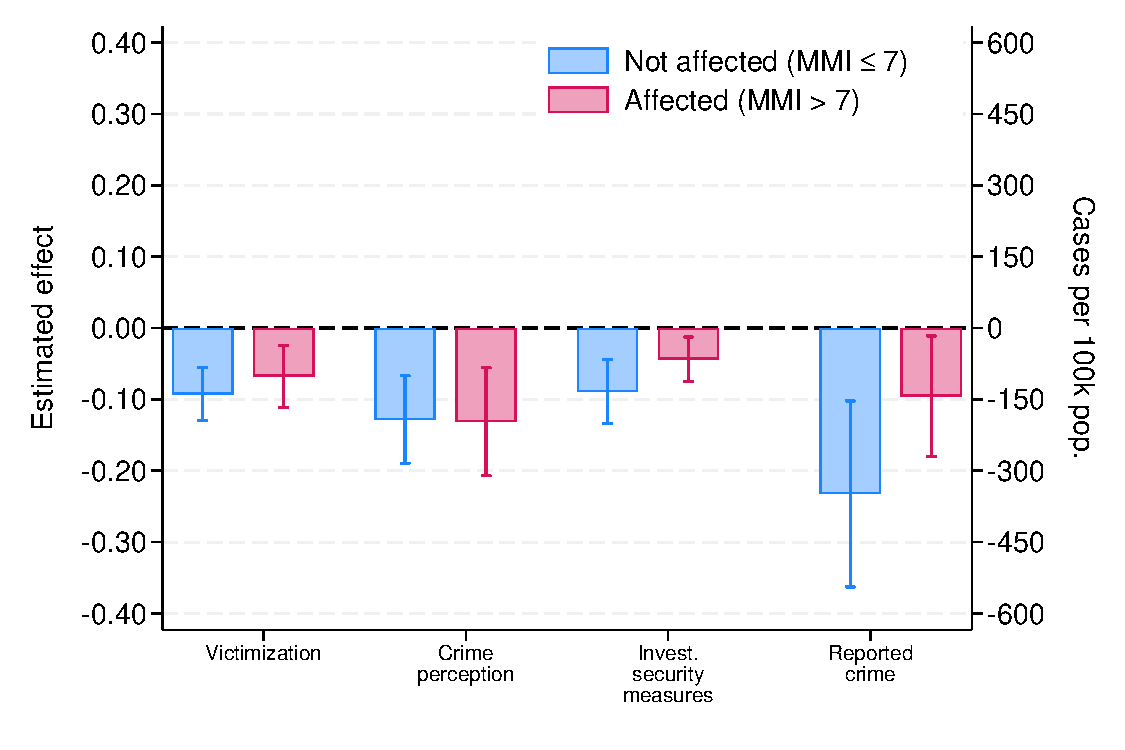
\includegraphics[width=0.8\textwidth]{../manuscript/Graphs/heterogeneity_earthquake_mmi.pdf}
    \\[10pt]
    \begin{minipage}{0.99\textwidth}
    \footnotesize
    Notes: This figure reports the heterogeneous effects of \emph{Plan Cuadrante} by exposure to the 2010 Maule earthquake, estimated separately for municipalities more exposed to the earthquake---defined as those with a Modified Mercalli Intensity (MMI) greater than 7, ``affected'' (red bars)---and municipalities with an MMI of 7 or lower (``not affected'', blue bars), using all adopters. For each exposure group, we estimate the pooled post-treatment effect of the program with the difference-in-differences estimator for staggered adoption of \citet{Callaway}, comparing municipalities of the same exposure level to each other so that the earthquake's direct effect on outcomes is differenced out within each group. Victimization is the probability of household victimization in the last 12 months; crime perception is the probability of perceiving an increase in crime; and investment in security measures is the probability of adopting security measures in the last twelve months---all from the ENUSC survey and read on the left axis. Reported crime is the number of crimes reported to the police per 100,000 inhabitants, from administrative data, and read on the right axis. Bars represent the average post-treatment effect and the whiskers the 95\% confidence intervals; standard errors are clustered at the municipality level using the wild bootstrapping procedure.
    \end{minipage}
\end{figure}
}
\end{center}


\clearpage 
\end{response}
\stepcounter{AnsweredComments}

\begin{refcomment}
\smallskip

4. In addition, to assess the impacts of the reform the authors look at the effects on the perceptions of police performance by comparing perceptions between early and late adopters (Figure 4). To interpret this exercise, it would first be necessary that the authors provide evidence that adoption timing was not driven by differences in other pre-policy changes in local outcomes. Even if not all survey questions are available in every year, a regression of outcomes on the number of years of exposure to the policy could provide an alternative way to address this.

\label{pt:r1_06}
\end{refcomment}

% Our reply to R1 - 6 
\begin{response}
	%2.4 In addition, to assess the impacts of the reform the authors look at the effects on the perceptions of police performance by comparing perceptions between early and late adopters (Figure 4). To interpret this exercise, it would first be necessary that the authors provide evidence that adoption timing was not driven by differences in other pre-policy changes in local outcomes. Even if not all survey questions are available in every year, a regression of outcomes on the number of years of exposure to the policy could provide an alternative way to address this.

This is an excellent point, thank you very much. The reviewer noted that, to interpret this exercise, it would be necessary to show that adoption timing was not driven by differences in other pre-policy changes. Following reviewer's suggestion, we regress perceived police performance outcomes on the year of adoption of \emph{Plan Cuadrante}, restricting the sample to municipalities that had not yet adopted the program as of 2005, the year for which information on perceived police performance is available. The results, reported in panel (a) of Figure \ref{fig:balance_doseresponse}, show that perceived police performance before \emph{Plan Cuadrante} did not predict the timing of adoption.


Following your suggestion, as an additional exercise, we also reestimate the comparison reported in panel (a) of Figure 4, measuring years of exposure to \emph{Plan Cuadrante} in 2005 rather than simply whether the municipality had adopted the program. The results, reported in panel (b) of Figure \ref{fig:balance_doseresponse}, show the expected correlations, consistent with an increasing effect of \emph{Plan Cuadrante} on perceived police performance.

We have included the following footnote in Section 4.4 of the manuscript to reference these results:

\begin{adjustwidth}{2em}{0em}
Information on police performance is only available in ENUSC round 2005. Using this round, we compare perceived police performance in municipalities that adopted \emph{Plan Cuadrante} in 2005 or earlier and in municipalities adopting after 2005. Figure \ref{fig:balance_doseresponse} in Online Appendix \ref{sec:appendixB} shows that the number of years of exposure to \emph{Plan Cuadrante} is positively correlated with perceived police performance. While these exercises on perceived police performance should be interpreted with caution, we show in the same appendix that the timing of future adoption is not correlated with perceived police performance in 2005 for municipalities that had not yet adopted the program by 2005.
\end{adjustwidth}

And we added the following subsection, ``Adoption Timing and Perceived Police Performance,'' to Online Appendix B reporting this exercise in detail:

\begin{adjustwidth}{2em}{0em}
Information on perceived police performance is only available in the 2005 round of ENUSC, so the comparison in Figure \ref{fig:figure05} relies on a single cross-section, comparing municipalities that had already adopted \emph{Plan Cuadrante} by 2005 (early adopters) with those that had not yet done so (late adopters). We consider seven measures of perceived police performance: the share of respondents who perceive police performance as good, and who perceive the police to be efficient, helpful, well informed, corrupt, failing to control crime, and failing to do their job well.

We start by assessing whether adoption timing is correlated with police performance. Using the sample of municipalities that introduced \emph{Plan Cuadrante} after 2005, Panel (a) of Figure \ref{fig:balance_doseresponse} examines the correlation between adoption timing and perceived police performance in 2005. The estimated coefficients are close to zero and statistically insignificant at conventional confidence levels, indicating that how soon a not-yet-treated municipality would go on to adopt the program is unrelated to its perceived police performance before treatment.

In Panel (b) of Figure \ref{fig:balance_doseresponse} we re-estimate the analysis conducted in Figure \ref{fig:figure05} but measuring years of exposure to \emph{Plan Cuadrante} in 2005 rather than simply whether they have adopted it or not. The results are qualitatively similar to those estimates reported in Figure \ref{fig:figure05}, showing strong correlations between years of exposure to \emph{Plan Cuadrante} and perceived police performance.
\end{adjustwidth}

\clearpage
\noindent\textbf{Other figures referenced above:}
\vspace{0.5em}

{\setcounter{figure}{3}\renewcommand{\thefigure}{\arabic{figure}}
%--- Implementation
\begin{figure}[!ht]
    \centering
    \caption[\emph{Plan Cuadrante} and Changes in Police Performance]{\emph{Plan Cuadrante} and Changes in Police Performance}
    \label{fig:figure05}
    \label{fig:police_performance}
    \label{fig:effectiveness_es}
    \begin{subfigure}[t]{0.44\textwidth}
        \centering
        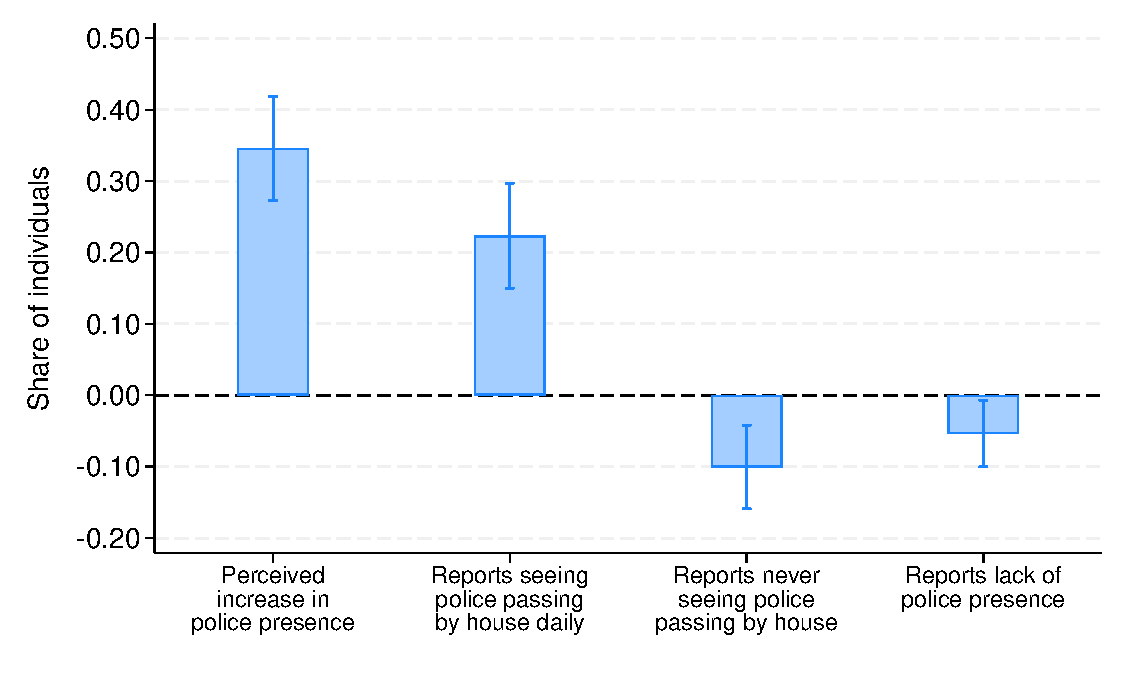
\includegraphics[width=\linewidth]{../manuscript/Graphs/results_policepresence.pdf}
        \caption{Effect on police presence}
    \end{subfigure}\hfill
    \begin{subfigure}[t]{0.44\textwidth}
        \centering
        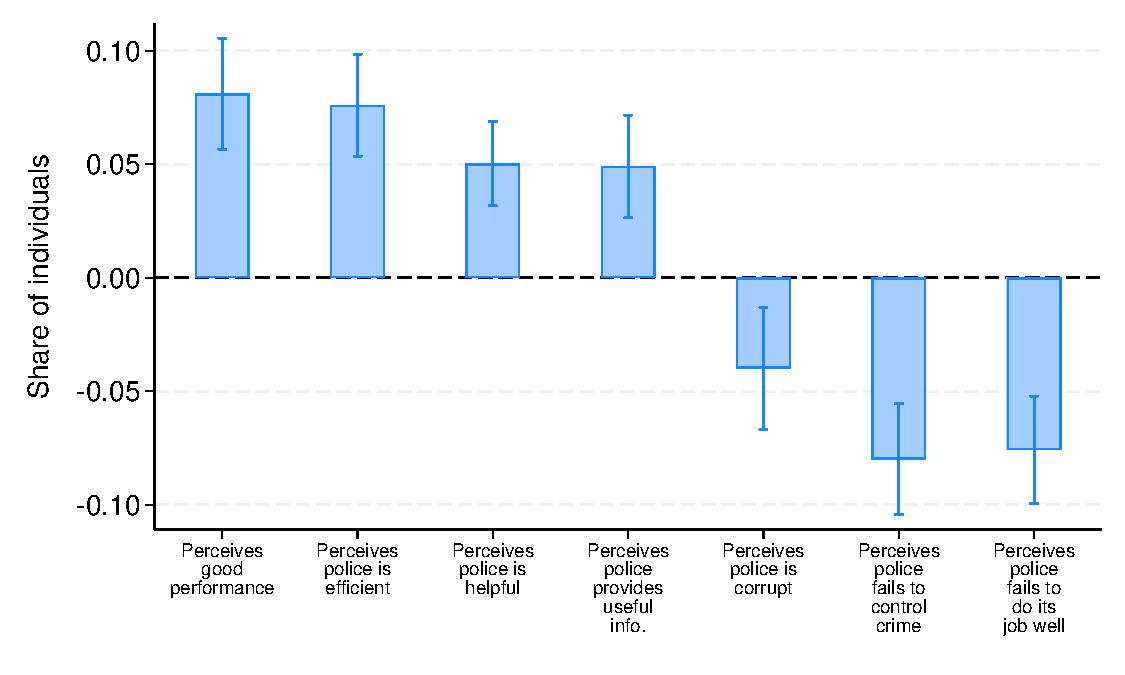
\includegraphics[width=\linewidth]{../manuscript/Graphs/combined_PCttest_2.pdf}
        \caption{Effect on perceived police performance}
    \end{subfigure}
    \\[6pt]
    \begin{subfigure}[t]{0.44\textwidth}
        \centering
        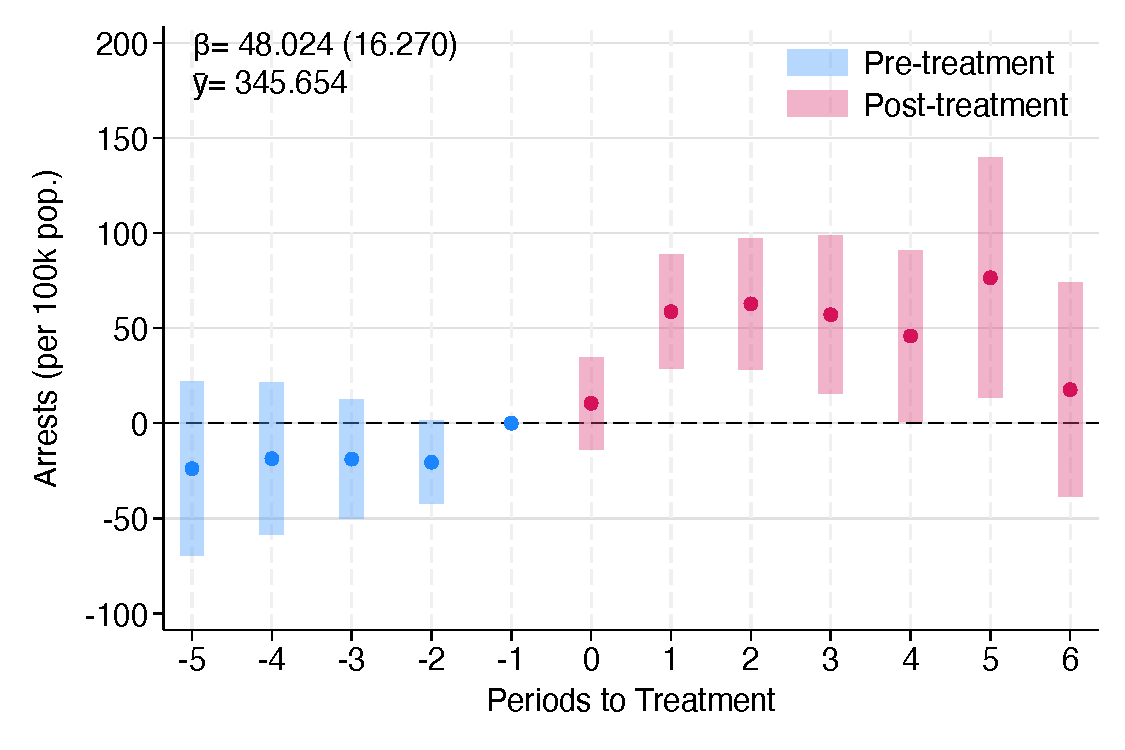
\includegraphics[width=\linewidth]{../manuscript/Graphs/totalarrestscrime_allcomunas.pdf}
        \caption{Arrests (per 100k pop.)}
    \end{subfigure}\hfill
    \begin{subfigure}[t]{0.44\textwidth}
        \centering
        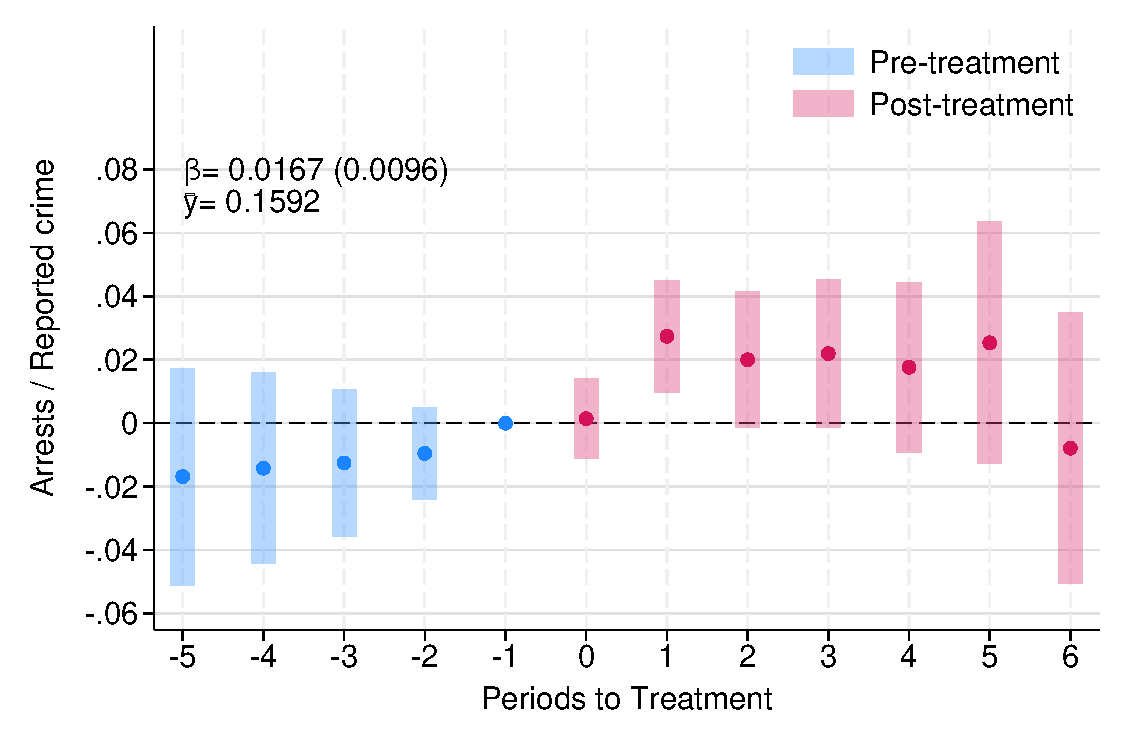
\includegraphics[width=\linewidth]{../manuscript/Graphs/arrests_over_reportedcrime_allcomunas.pdf}
        \caption{Arrests / Reported crime}
    \end{subfigure}
    \\[6pt]
    \begin{subfigure}[t]{0.44\textwidth}
        \centering
        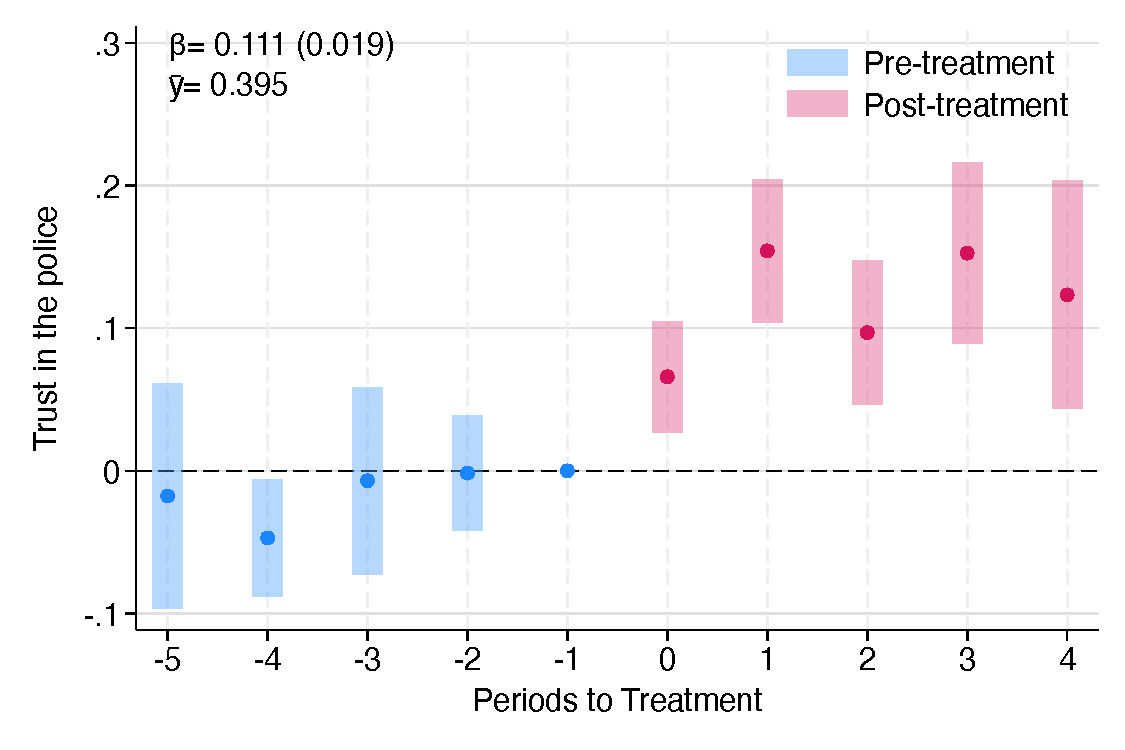
\includegraphics[width=\linewidth]{../manuscript/Graphs/results_trustcarabineros.pdf}
        \caption{Trust in the police}
    \end{subfigure}
    \\[8pt]
    \begin{minipage}{0.99\textwidth}
    \footnotesize Notes: Panel (a) reports the effects on perceived police presence. Panel (b) reports perceived police performance in 2005, comparing municipalities where \emph{Plan Cuadrante} was already implemented before 2006 with municipalities where it was implemented after 2005. Panels (c), (d), and (e) report dynamic event-study estimates for arrests per 100,000 inhabitants, the ratio of arrests to reported crime, and trust in the police. The estimation follows \citet{Callaway}. The graphs display estimated coefficients and 95\% confidence intervals. Standard errors are clustered at the municipality level using the wild bootstrapping procedure.
    \end{minipage}
\end{figure}
}

\clearpage

{\renewcommand{\thefigure}{B.6}
\begin{figure}[H]
    \centering
    \caption{Timing of Adoption of \emph{Plan Cuadrante} and Perceived Police Performance}
    \label{fig:balance_doseresponse}
    \begin{subfigure}{0.495\textwidth}
        \centering
        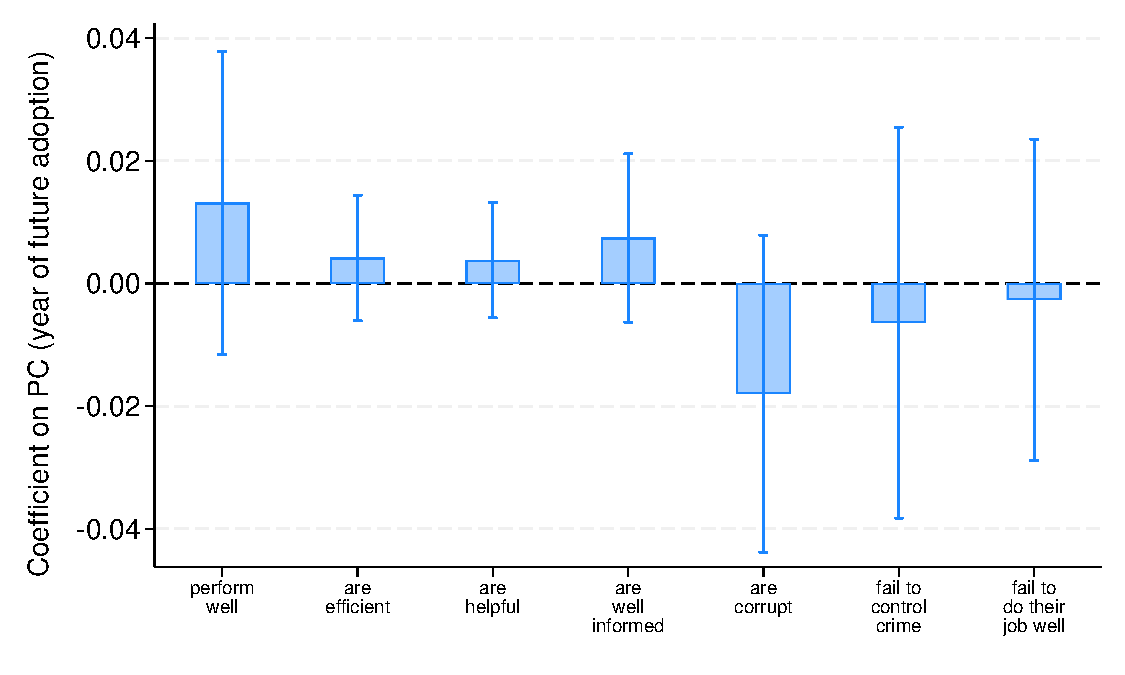
\includegraphics[width=\textwidth]{../manuscript/Graphs/balance_carabperc.pdf}
        \caption{Year of adoption and police performance before adoption}
    \end{subfigure}%
    ~
    \begin{subfigure}{0.495\textwidth}
        \centering
        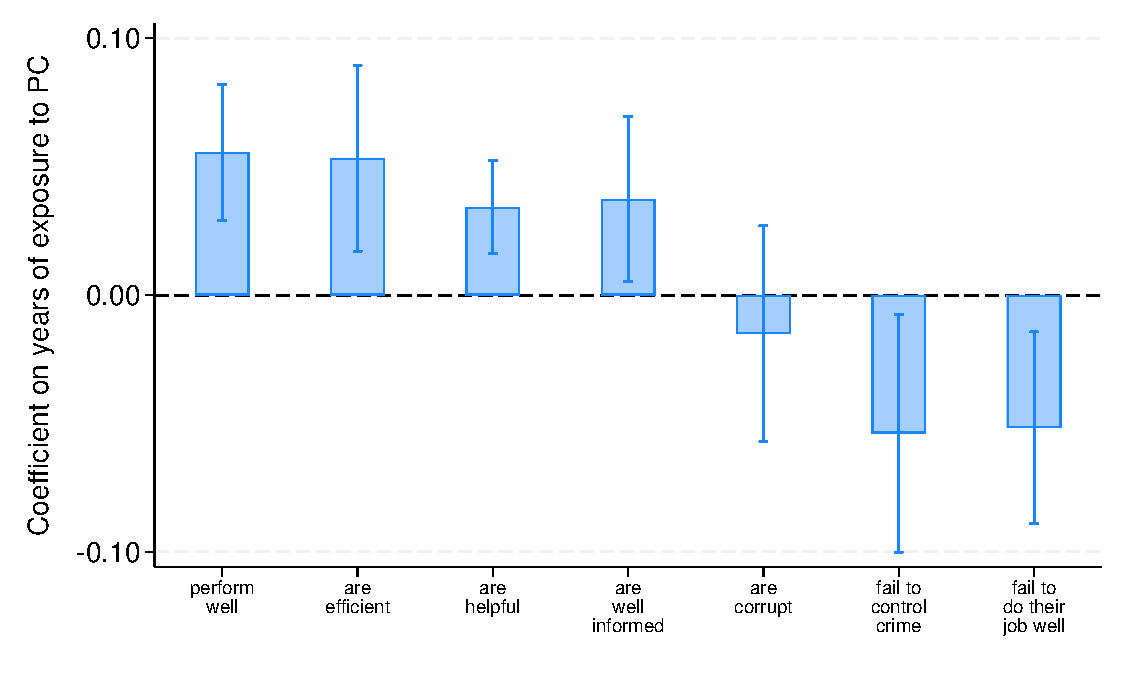
\includegraphics[width=\textwidth]{../manuscript/Graphs/doseresponse_carabperc.pdf}
        \caption{Years exposed to \emph{Plan Cuadrante} (dose response)}
    \end{subfigure}%
    \\[12pt]
    \begin{minipage}{0.99\textwidth}
    Notes: The figure considers seven measures of police performance: the share of respondents who perceive police performance as good, and who perceive the police to be efficient, helpful, well informed, corrupt, failing to control crime, and failing to do their job well. Using the sample of municipalities that adopted \emph{Plan Cuadrante} after 2005, panel (a) examines whether the future timing of adoption of \emph{Plan Cuadrante} is correlated with perceived police performance in 2005, before the introduction of the program. Panel (b) reestimates the same comparison as Figure \ref{fig:figure05}, replacing the binary adoption indicator with the municipality's number of years of exposure to \emph{Plan Cuadrante} as of 2005. In both panels, each bar plots the coefficient from a separate regression of one performance measure. The graphs display the estimated coefficients and 95\% confidence intervals.
    \end{minipage}
\end{figure}
}

\clearpage

 
\end{response}
\stepcounter{AnsweredComments}

\begin{refcomment}
\smallskip

\textbf{Contribution}: Once the ingredients of the policy are clarified, the paper’s contribution should be expanded, because at present it does not fully engage with the most recent literature. Beyond the large body of work on police size and crime, a few recent papers have examined how the allocation of police resources across space and time affects police effectiveness (among others, Adda et al. (2014), Blanes i Vidal and Mastrobuoni (2018), Mastrobuoni (2019, 2020)). Furthermore, it should also connect more explicitly with the growing body of work on the impact of policing on community-related outcomes such as trust, perceptions, and willingness to cooperate (e.g. Blanco et al. (2013), Ang et al. (2025), Facchetti (2025), Gonçalves et al. (2025)).

I appreciate the effort to relate to work that inform how to organize state presence in space. However, to make this a convincing contribution, the authors would need to discuss explicitly whether centralizing policing over a larger jurisdiction improves the allocation of resources compared to spreading them, and I am not sure if they can currently do it. A cost-benefit analysis, or even a marginal value of public funds (MVPF) estimate, could help.


\label{pt:r1_07}
\end{refcomment}

% Our reply to R1 - 7 
\begin{response}
	%% Comment 3: 3.	Contribution
%Once the ingredients of the policy are clarified, the paper’s contribution should be expanded, because at present it does not fully engage with the most recent literature. Beyond the large body of work on police size and crime, a few recent papers have examined how the allocation of police resources across space and time affects police effectiveness (among others, Adda et al. (2014), Blanes i Vidal and Mastrobuoni (2018), Mastrobuoni (2019, 2020)). Furthermore, it should also connect more explicitly with the growing body of work on the impact of policing on community-related outcomes such as trust, perceptions, and willingness to cooperate (e.g. Blanco et al. (2013), Ang et al. (2025), Facchetti (2025), Gonçalves et al. (2025)).

%I appreciate the effort to relate to work that inform how to organize state presence in space. However, to make this a convincing contribution, the authors would need to discuss explicitly whether centralizing policing over a larger jurisdiction improves the allocation of resources compared to spreading them, and I am not sure if they can currently do it. A cost-benefit analysis, or even a marginal value of public funds (MVPF) estimate, could help.


Thank you for these suggestions. We have read all the cited studies carefully and agree that they are highly relevant and should have been included in our discussion. They are now integrated into the motivation of the paper.

\citet{Adda_etal_2014}, \citet{Blanes_Mastrobuoni_2018}, \citet{MASTROBUONI2019}, \citet{facchetti2025}, and \citet{Mastrobuoni_2020} were particularly helpful in sharpening our understanding of how the allocation of police resources and efforts across space, time and crimes affects policing outcomes and public safety, the mechanisms driving these effects, and of the role that technology can play in improving police effectiveness. We now engage more explicitly with this literature when discussing the contributions of our results.

\citet{Blanco_2025} and \citet{ang_etal_2025} helped us better motivate the importance of community trust in the police, its drivers, and how it shapes policing outcomes, and \citet{Goncalves_etal_2025} documented police misconduct. We now connect our findings more explicitly to this growing literature, highlighting how the intervention we examine can increase trust in the police and the beneficial secondary effects of it. 


Below are the paragraphs in the updated introduction where we have integrated the relevant literature and highlighted the contributions of our results: 

\begin{adjustwidth}{2em}{0em}

Our findings contribute to two related strands of the literature on police organization and public safety. First, they provide some of the first causal evidence on the effects of beat policing on crime and security perceptions. Beat policing has become one of the most widely adopted policing models globally \citep{NASEM2018,PCSP2014}, yet robust causal evidence on its effectiveness remains scarce. We show that this model can generate substantial reductions in crime victimization, reported crime, and insecurity perceptions.

These results also speak to recent work on other policing models. Hot-spot policing reallocates police resources toward high-crime locations and has been shown to reduce crime in targeted areas, though often with displacement to nearby places \citep{DiTella, Blattman_Tobon_JEEA, Draca_2011, Weisburd_restat}. Beat policing differs fundamentally. Rather than concentrating police presence in selected locations---where the same officers need not return repeatedly---it provides continuous, territory-wide coverage through permanent officer-to-area assignment. This distinction matters in our setting, where many quadrants were not crime hot spots and the reform generated municipality-wide declines in crime and insecurity perceptions, with no evidence of spillovers to neighboring municipalities. Community policing, another model that has received growing attention in the economics literature, emphasizes citizen participation in defining policing priorities and, in some cases, in implementation itself. While it has been shown to increase trust in police in developed countries, evidence from low- and middle-income settings points to more limited effects on crime and trust \citep{blair2021, Tobon}. Beat policing also differs from that approach. By permanently assigning officers to stable territorial units, it strengthens local knowledge and brings police closer to communities without requiring direct citizen participation in strategy or operations. Our findings show that this model can reduce crime and insecurity perceptions while increasing trust in police institutions in a middle-income country.

A second contribution is to the broader literature showing that specific features of police organization matter for police effectiveness and public security outcomes. Research has shown that faster police response times improve crime clearance \citep{Blanes_Kirchmaier}, that the effectiveness of police presence depends on how this is organized and deployed rather than simply on their intensity \citep{facchetti2025, MASTROBUONI2019, Blanes_Mastrobuoni_2018}, that shifts in police prioritization across crime types shape criminal behavior \citep{Adda_etal_2014}, and that better information systems and technology can improve police performance \citep{Mastrobuoni_2020}. Earlier work also found that areas covered by smaller, more localized police departments outperform, in terms of security, those covered by larger centralized ones, hypothesizing that this might be related, among other factors, to closer citizen-police engagement \citep{ostrom1973, ostrom1978}. We add to this literature by studying a policing model that combines several of these margins within a single organizational reform. By assigning officers permanently to smaller territorial units rather than rotating them across larger ones, beat policing is designed to increase police visibility, strengthen knowledge of local conditions, and improve the capacity of officers to adapt their practices to local crime patterns. In line with these mechanisms, we show that the adoption of \emph{Plan Cuadrante} increased perceived police presence in neighborhoods and raised police effectiveness, as arrests increased even while victimization and reported crime declined. These organizational improvements translated into meaningful gains in public safety and security perceptions.

A third contribution concerns the literature on police resources, which documents elasticities of crime with respect to officers and expenditure ranging from $-0.1$ to $-2$, with larger effects in developed settings and for violent crimes \citep{Chalfin_JEL, Levitt_1997, DiTella}. We complement this body of work by showing that the quantity of resources is not the only margin that matters. How those resources are deployed matters as well. \emph{Plan Cuadrante} improved public safety outcomes even in municipalities that experienced no increase in police resources relative to controls, suggesting that reorganizing deployment can raise public safety and police effectiveness without expanding the resource base.

We also contribute to the literature on police practices, institutional trust, and citizen cooperation. A persistent challenge is that security perceptions often diverge from actual crime trends \citep{ajzenman2022}, limiting the scope for improving both simultaneously. Rising crime erodes institutional trust \citep{Blanco_2025}, while police misconduct undermines cooperation \citep{ang_etal_2025}.\footnote{Racial disparities in police behavior are also well documented; see, e.g., \citet{Goncalves_etal_2025}, who develop a method to correct for selection bias in estimates of racial disparities in the use of force.} Our results show that beat policing can improve both dimensions---security and security perceptions---by bringing officers into sustained engagement with local communities through permanent territorial assignment. We document not only increases in police trust and evaluations of police performance, but also substantial reductions in private security investment, indicating that households revised their threat assessments in response to the program. 

Finally, our findings speak to a broader question about how organizational design shapes public-service effectiveness. A growing literature shows that the spatial organization of service provision matters. In policing, we show that a model organizing officers around fixed territorial units---allowing them to build local knowledge, coordinate with local actors, and adapt practices accordingly---can substantially improve both crime control and institutional legitimacy. This aligns with evidence from health and education showing that bringing providers closer to the populations they serve can improve outcomes \citep{besley2003centralized, Bardhan, Bloom_2015, Basurto}. In a rigorously identified setting, we show that this type of organizational proximity generates meaningful gains in police effectiveness and citizen security.

\end{adjustwidth}


Regarding the connection of our results with the literature on state service provision organization, we agree that addressing whether centralizing policing over a larger jurisdiction—or, alternatively, spreading officers across smaller, fixed territorial units—improves the allocation of police resources is central to the contribution of the paper. Our findings speak directly to this question. The organizational logic of \emph{Plan Cuadrante} is precisely one of territorial or local specialization: rather than maintaining a centralized dispatch model in which officers patrol in rotation large, undifferentiated areas, the reform assigns officers permanently to small, fixed quadrants, enabling them to build local knowledge and adapt their practices to local crime patterns. Municipalities receiving large increases in police officers and patrol vehicles experienced improvements in victimization similar to those in municipalities receiving resource increases similar to control, indicating that the scale of resource infusion alone does not drive effectiveness. This result supports the view that the organizational model---with permanent assignment to small territorial  areas--- is a key driver of effectiveness. While our design does not allow a direct budget-constrained comparison between a centralized rotating model and a beat policing model, these findings suggest that spreading officers across smaller fixed units, as \emph{Plan Cuadrante} does, generates efficiency gains in resource allocation.

Regarding the request for a cost-benefit analysis or an MVPF estimate, we agree that this would be valuable in principle, but we do not think we can credibly implement it with the data currently available. On the cost side, the budget documents we were able to access (including Budget Office reports) do not cleanly separate baseline police expenditure that would have occurred in the absence of \emph{Plan Cuadrante} from the truly incremental expenditure required to implement and operate the reform. On the benefit side, we also lack a credible context-specific willingness-to-pay measure that would allow us to monetize the welfare gains from the observed reductions in victimization and insecurity. These limitations rule out a credible cost-benefit or MVPF calculation.

That said, an important feature of our setting is that \emph{Plan Cuadrante} is fundamentally an organizational reform of police deployment. Many municipalities that adopted the program experienced resource increases similar to those observed in control municipalities, suggesting that a substantial part of those resources would likely have been deployed even without the reform. In this sense, the gains associated with the beat-policing component are largely linked to how existing police capacity is organized and deployed across territory, rather than to large additional spending above the cost of maintaining a police force. We therefore interpret our findings as evidence that organizational redesign can generate sizeable improvements in public safety even when incremental budgetary costs are limited.


 
\end{response}
\stepcounter{AnsweredComments}

\begin{refcomment}
\smallskip

\textbf{Mechanisms}: I encourage the authors to expand the discussion of mechanisms, that at present is not very well developed. First, the authors should be explicit on what they mean with “police effectiveness”. Typically, effectiveness is proxied by arrests or clearance rates. This would also help separate two channels: deterrence and police effectiveness. Deterrence would change the incentives to commit crime, and thus would be reflected in reductions in crime, whereas the latter would be reflected in the ability of the police to deal with crime, which would show up in arrests conditional on crime. Furthermore, to shed light on this, it would be useful to consider whether the reform affected response times, patrolling patterns, or any other proxies that capture the ability of the police to solve crime, such as improved technology. An alternative channel is that the reform increased the salience of policing and thus raised citizen awareness. For instance, was the policy advertised? Of course, these mechanisms are not mutually exclusive, and I recognize that disentangling them empirically may be difficult, but a more systematic discussion would be very valuable.

\label{pt:r1_08}
\end{refcomment}

% Our reply to R1 - 8 
\begin{response}
	%% Comment 4:	Mechanisms

%I encourage the authors to expand the discussion of mechanisms, that at present is not very well developed. First, the authors should be explicit on what they mean with “police effectiveness”. Typically, effectiveness is proxied by arrests or clearance rates. This would also help separate two channels: deterrence and police effectiveness. Deterrence would change the incentives to commit crime, and thus would be reflected in reductions in crime, whereas the latter would be reflected in the ability of the police to deal with crime, which would show up in arrests conditional on crime. Furthermore, to shed light on this, it would be useful to consider whether the reform affected response times, patrolling patterns, or any other proxies that capture the ability of the police to solve crime, such as improved technology. An alternative channel is that the reform increased the salience of policing and thus raised citizen awareness. For instance, was the policy advertised? Of course, these mechanisms are not mutually exclusive, and I recognize that disentangling them empirically may be difficult, but a more systematic discussion would be very valuable.

Thanks for the specific and clear guidance to improve the analysis of mechanisms.

We revised the manuscript so that the mechanism discussion now distinguishes more clearly between deterrence and police effectiveness as two conceptually distinct but empirically intertwined channels through which beat policing may improve public safety and security perceptions. In the revised framing, police effectiveness is no longer used as a label for the main outcomes; instead, it refers to the capacity of police to prevent and resolve crime. In practice, with our data we cannot cleanly separate how much of the total effect comes from each channel, because they can reinforce each other: stronger preventive action and higher police presence can deter crime, and improved capacity to solve crimes can also deter crime by increasing the expected probability of apprehension; at the same time, lower crime incidence may allow police to concentrate effort on crime resolution. While we were not granted access to patrolling patterns or response times, we provide evidence consistent with both channels operating. Specifically, \emph{Plan Cuadrante} increases perceived police presence (Panel (a) of Figure \ref{fig:police_performance}), reduces household victimization and reported crime (Panels (a) and (b) of Figure \ref{fig:figure02}), increases arrests (Panel (c) of Figure \ref{fig:police_performance}), and increases arrests per reported crime (Panel (d) of Figure \ref{fig:police_performance}). The latter result should nonetheless be interpreted with caution, as the composition of reported crimes may also change with the program, affecting the ratio independently of any change in police effectiveness. Accordingly, in Section 4.4 the focus is not to isolate deterrence from effectiveness, but to disentangle which components of \emph{Plan Cuadrante}---resources, territorial deployment, and policing strategy---are most likely to explain the effects we document.

Regarding the possibility that the reform was accompanied by an advertisement campaign that increased the salience of policing and raised citizen awareness, we believe this is unlikely for two reasons. First, \emph{Plan Cuadrante} was an internal operational reform of Carabineros with no formal public communication component in its design. While the program received some media attention when it was broadly rolled out across Santiago in 2000, we find no evidence of targeted information campaigns at the municipality level when individual municipalities subsequently joined the program, and the staggered rollout over more than a decade makes a sustained media salience mechanism implausible. Second, and more importantly, if the improvement in crime were driven by media coverage or information campaigns, one would expect the effects to be concentrated shortly after adoption and to fade over time. Instead, the dynamic estimates show that the effects for most outcomes grow and persist over time.


Below we provide the updated mechanism section:

\begin{adjustwidth}{2em}{0em}
{\setcounter{figure}{3}\renewcommand{\thefigure}{\arabic{figure}}
%\textbf{4.4 What Is Driving the Effects of \emph{Plan Cuadrante}?}


To reduce crime and improve security perceptions, police forces need to strengthen both prevention and police effectiveness. Both margins can be shaped by resources, territorial deployment, and policing strategy. This section examines which components of \emph{Plan Cuadrante} are most likely to drive the effects documented in Section \ref{results}. 

The central objective of \emph{Plan Cuadrante} was to introduce a beat policing model by reorganizing deployment. Police operational territories that had typically matched municipal boundaries were subdivided into quadrants, and officers were permanently assigned to these quadrants. During our study period, national operational guidelines remained the same in adopting and non-adopting municipalities. Still, this new deployment likely affected policing strategy at a more operational level, because it allowed officers to adapt patrol routes, schedules, and prevention practices using the local knowledge that the program sought to build.

Although changes in resources were not the core of the reform, implementation contemplated increases in municipalities that lacked the personnel and patrol capacity required to move to this model. During the period we study, Chile was expanding public spending on security, and police resources increased in most municipalities regardless of whether or when they adopted \emph{Plan Cuadrante}. On average, however, municipalities adopting the program experienced larger increases in officers and patrol vehicles, as shown in panels (a) and (b) of Figure \ref{fig:resources}. Since increases in police resources have been shown to reduce crime in some contexts \citep{Evans}, this pattern raises a central question for interpretation, namely whether our estimates reflect resource expansion or the deployment and strategy changes introduced by \emph{Plan Cuadrante}. We address this question through a set of exercises that exploit heterogeneity in resource increases across municipalities and over time.

\FloatBarrier
%--- Implementation
\begin{figure}[H]
    \centering
    \caption{Plan Cuadrante and Changes in Police Resources}
    \label{fig:resources}
    \label{fig:figure_resources}
    \begin{tabular}{cc}
        \begin{minipage}[t]{0.48\textwidth}
            \centering
            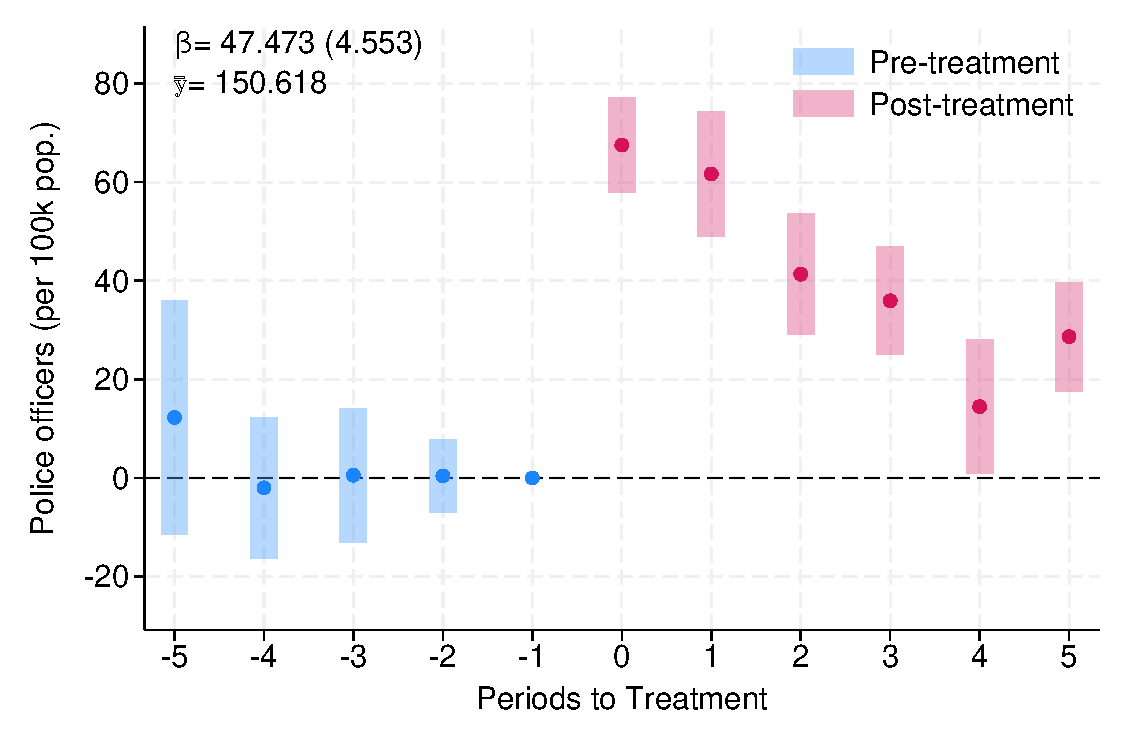
\includegraphics[width=\linewidth]{../manuscript/Graphs/fig4_officers.pdf}

            \small (a) Effect on the number of police officers
        \end{minipage}
        &
        \begin{minipage}[t]{0.48\textwidth}
            \centering
            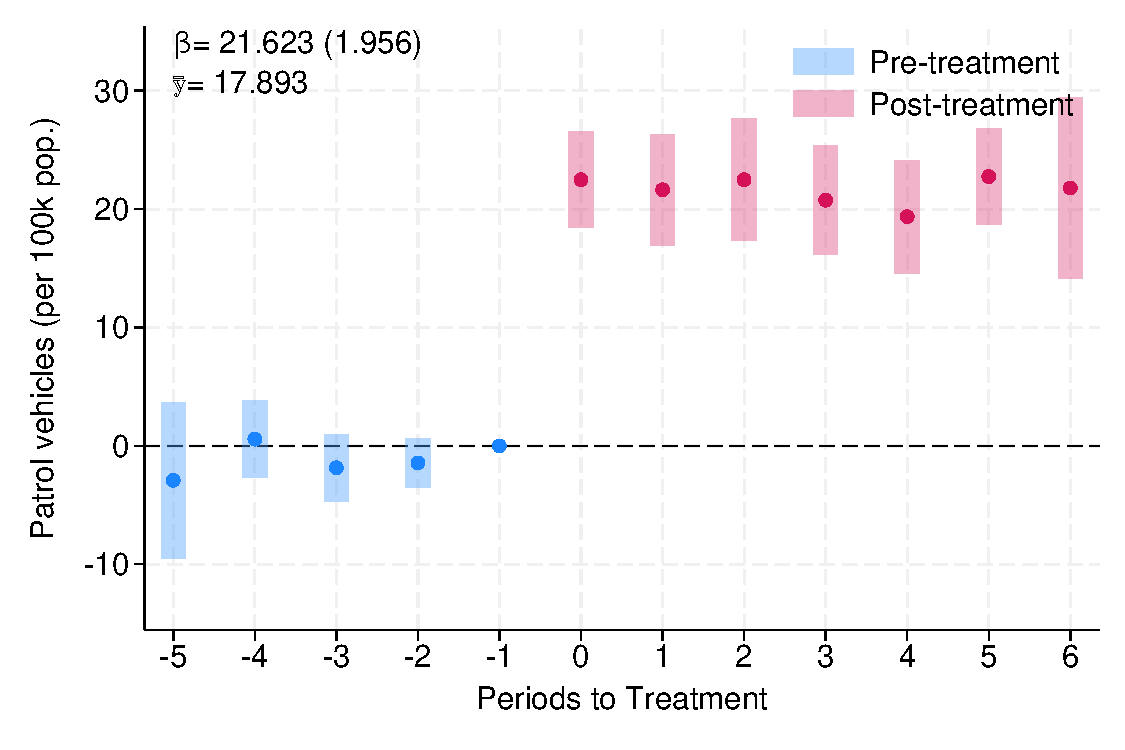
\includegraphics[width=\linewidth]{../manuscript/Graphs/fig4_patrols.pdf}

            \small (b) Effect on the number of patrol vehicles
        \end{minipage}
        \\[4pt]
        \begin{minipage}[t]{0.48\textwidth}
            \centering
            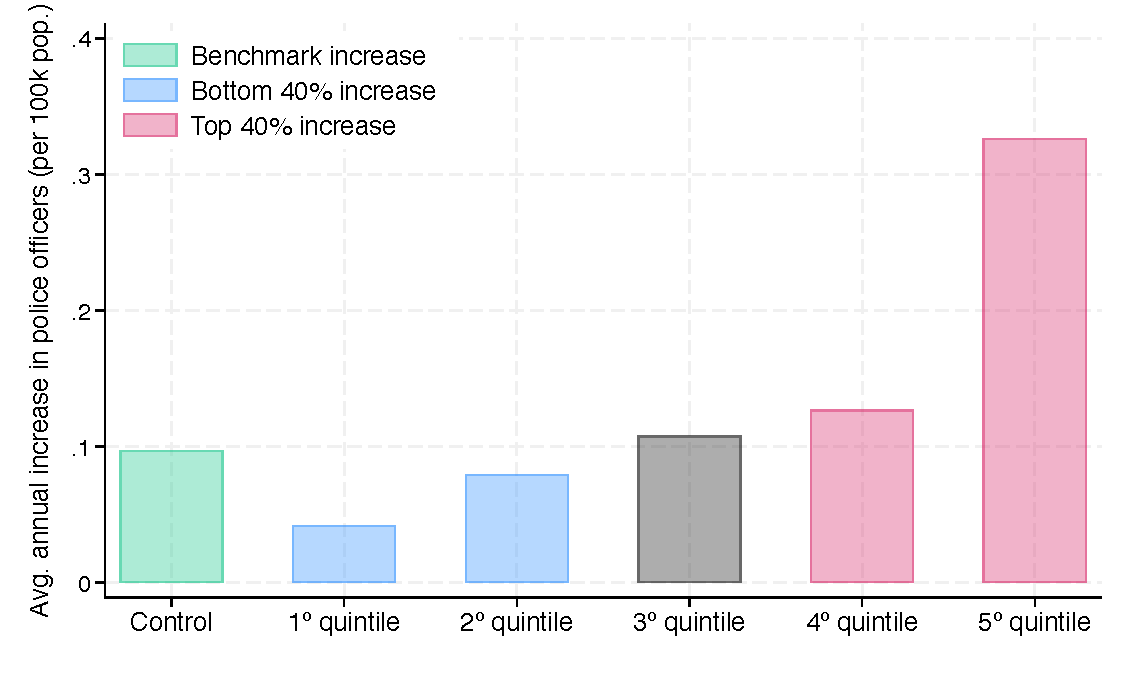
\includegraphics[width=\linewidth]{../manuscript/Graphs/increase_enusc_off_quintiles.pdf}

            \small (c) Distribution of $\Delta$ in police officers
        \end{minipage}
        &
        \begin{minipage}[t]{0.48\textwidth}
            \centering
            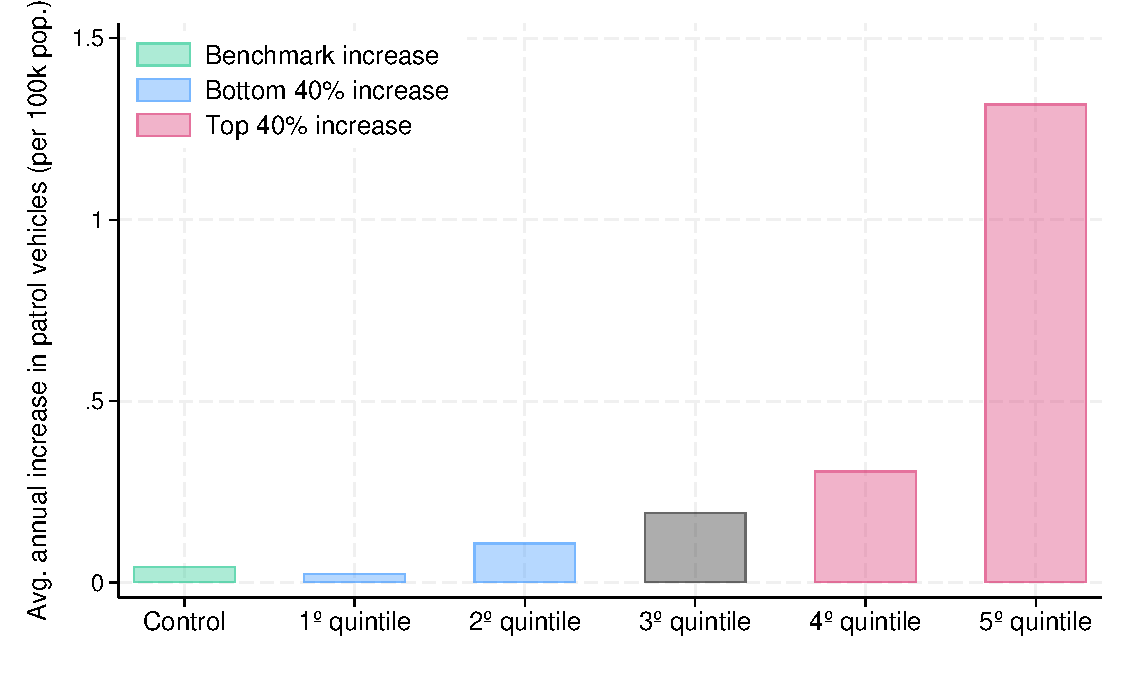
\includegraphics[width=\linewidth]{../manuscript/Graphs/increase_enusc_pv_quintiles.pdf}

            \small (d) Distribution of $\Delta$ in patrol vehicles
        \end{minipage}
        \\[4pt]
        \begin{minipage}[t]{0.48\textwidth}
            \centering
            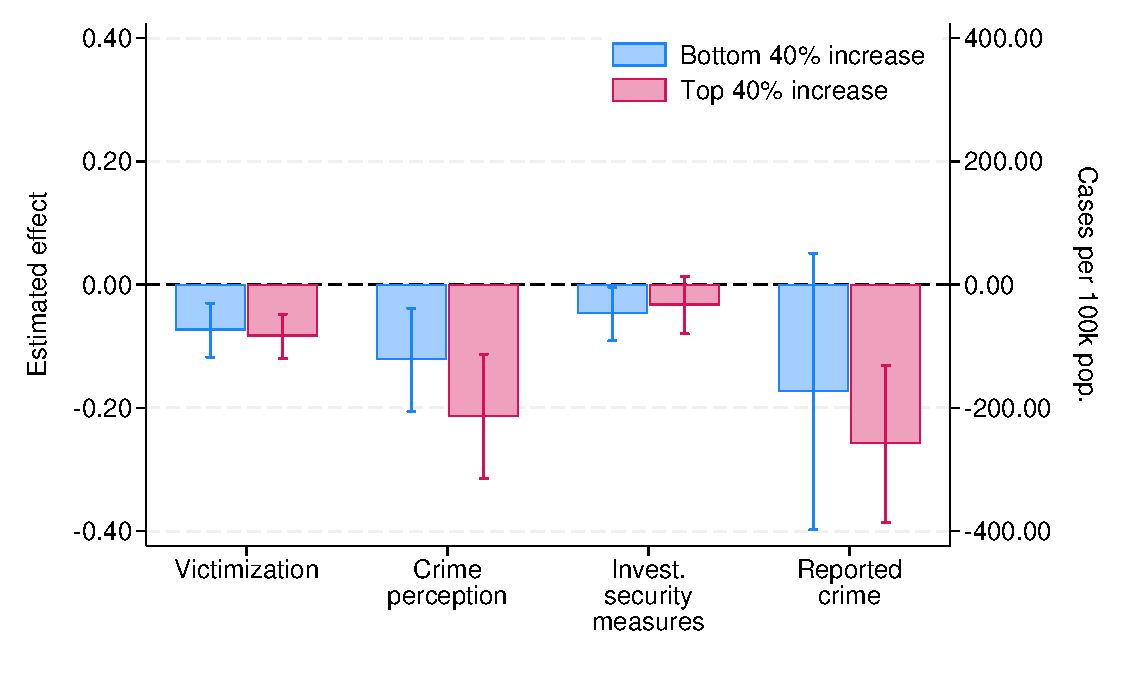
\includegraphics[width=\linewidth]{../manuscript/Graphs/heterogeneity_off.pdf}

            \small (e) Effects by the intensity of $\Delta$ in police officers
        \end{minipage}
        &
        \begin{minipage}[t]{0.48\textwidth}
            \centering
            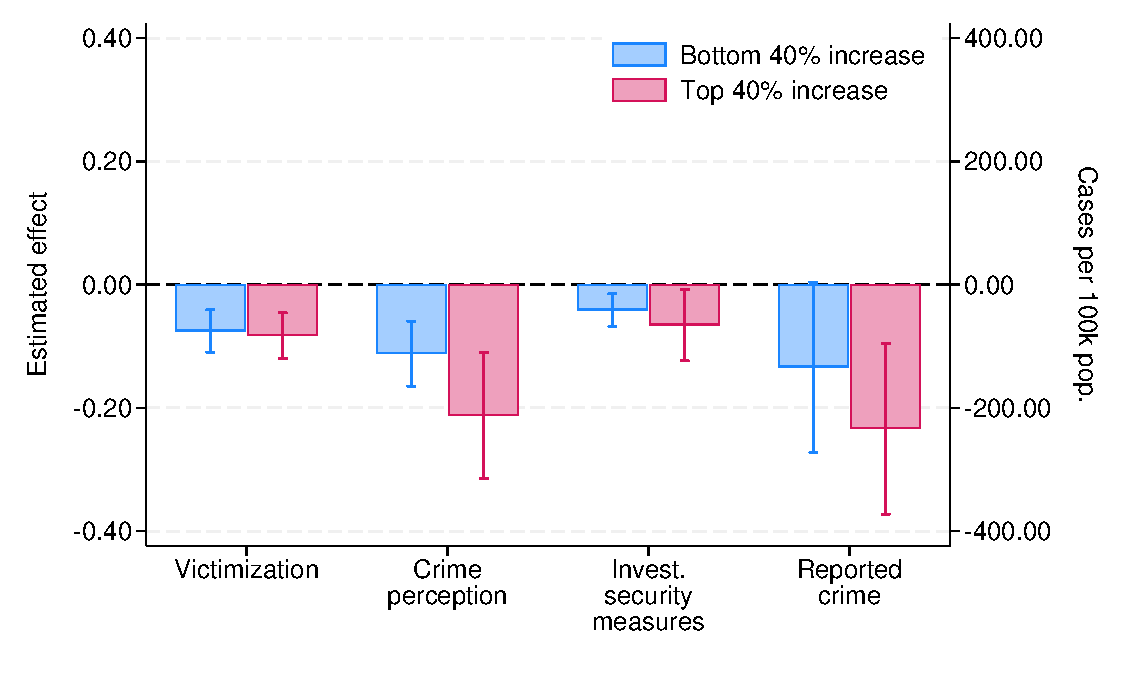
\includegraphics[width=\linewidth]{../manuscript/Graphs/heterogeneity_pv.pdf}

            \small (f) Effects by the intensity of $\Delta$ in patrol vehicles
        \end{minipage}
    \end{tabular}
    \vspace{4pt}
    \begin{minipage}{0.99\textwidth}
    \footnotesize Notes: Panels (a) and (b) show the effect of \emph{Plan Cuadrante} on police officers and patrol vehicles per 100,000 inhabitants. Panels (c) and (d) show the distribution of annual changes in officers and patrol vehicles across municipalities. Panels (e) and (f) report effects by the intensity of resource changes, comparing municipalities in the bottom 40\% and top 40\% of the distribution. The estimation follows \citet{Callaway}. The graphs display estimated coefficients and 95\% confidence intervals. Standard errors are clustered at the municipality level using wild bootstrapping.
    \end{minipage}
\end{figure}
\FloatBarrier
Panels (c) and (d) of Figure \ref{fig:resources} show that the average increase in police resources masks substantial heterogeneity. Municipalities in the bottom 40\% of the resource-change distribution (blue bars) experienced increases close to the average annual variation observed among never treated and not-yet-treated municipalities (green bar). By contrast, municipalities in the top 40\% (red bars) experienced much larger increases, with officers rising by around 22\% and patrol vehicles by around 80\%. If the effects of \emph{Plan Cuadrante} were driven by resource increases alone, we would not expect effects in municipalities whose resource increases were similar to those of the control group. Yet panels (e) and (f) of Figure \ref{fig:resources} show sizeable effects for most crime and crime-perception outcomes even in that low-increase group. While there may be a resource gradient for some crime-perception outcomes, the effects on twelve-month victimization and private investment in security among municipalities with control-like resource increases are close in magnitude to those in municipalities with larger increases. Reassuringly, municipalities in the top and bottom 40\% of the resource-increase distribution do not display differential pre-treatment trends in outcomes or police resources, which suggests that this heterogeneity is not driven by differential pre-existing trends.\footnote{We test for the joint significance of the pre-treatment coefficients between the two groups, separately for the split based on the increase in police officers and the split based on the increase in patrol vehicles. The resulting p-values are, respectively, 0.823 and 0.048 for victimization, 0.059 and 0.379 for crime perception, 0.820 and 0.157 for investment in security measures, and 0.213 and 0.419 for reported crime, as well as 0.616 and 0.444 for police officers and 0.405 and 0.157 for patrol vehicles.}

Although we cannot fully separate the beat policing component from the resource component of the reform---resources may have been important to enable effective implementation of the program, or may explain part of the effects in some municipalities---the fact that municipalities with resource increases similar to those experienced by control municipalities still display sizeable effects indicates that the effects of \emph{Plan Cuadrante} are not driven entirely by resources.\footnote{We also re-estimate the results in Figure \ref{fig:figure02} but controlling for police resources. Online Appendix Table \ref{tab:results_controlbyresources} shows that the magnitude of the estimated effects remains similar for most variables, although the statistical significance is reduced in some estimations. This likely reflects a mechanical feature of the \citet{Callaway} estimation procedure: control variables are not incorporated parametrically, but are instead used to construct the comparison group via outcome regression or propensity-score weighting, so the resulting estimation uncertainty propagates to the ATT standard errors. Note, in addition, that police resources are a bad control---i.e., at least part of their variation is a result of the adoption of \emph{Plan Cuadrante}---so these results should be interpreted cautiously.}\footnote{Table \ref{tab:resourcecorrelates} in Online Appendix \ref{sec:appendixB} examines which factors are associated with a larger increase in police resources upon the adoption of \emph{Plan Cuadrante}.}


\FloatBarrier
%--- Implementation
\begin{figure}[h!]
    \centering
    \caption{Police Resources and Public Safety}
    \label{fig:resources2}
    \begin{subfigure}[t]{0.55\textwidth}
        \centering
        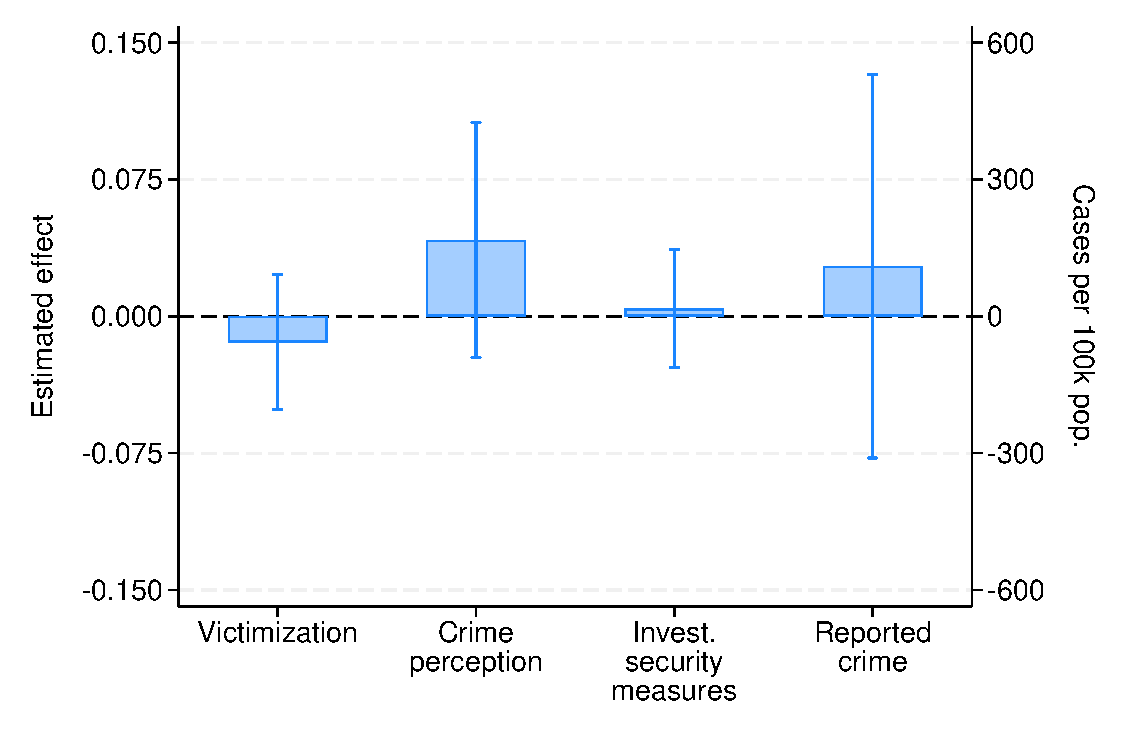
\includegraphics[width=\linewidth]{../manuscript/Graphs/results_SC_att_combined.pdf}
        \caption{Effects of \emph{Seguridad Ciudadana}}
    \end{subfigure}
    \\[6pt]
    \begin{subfigure}[t]{0.55\textwidth}
        \centering
        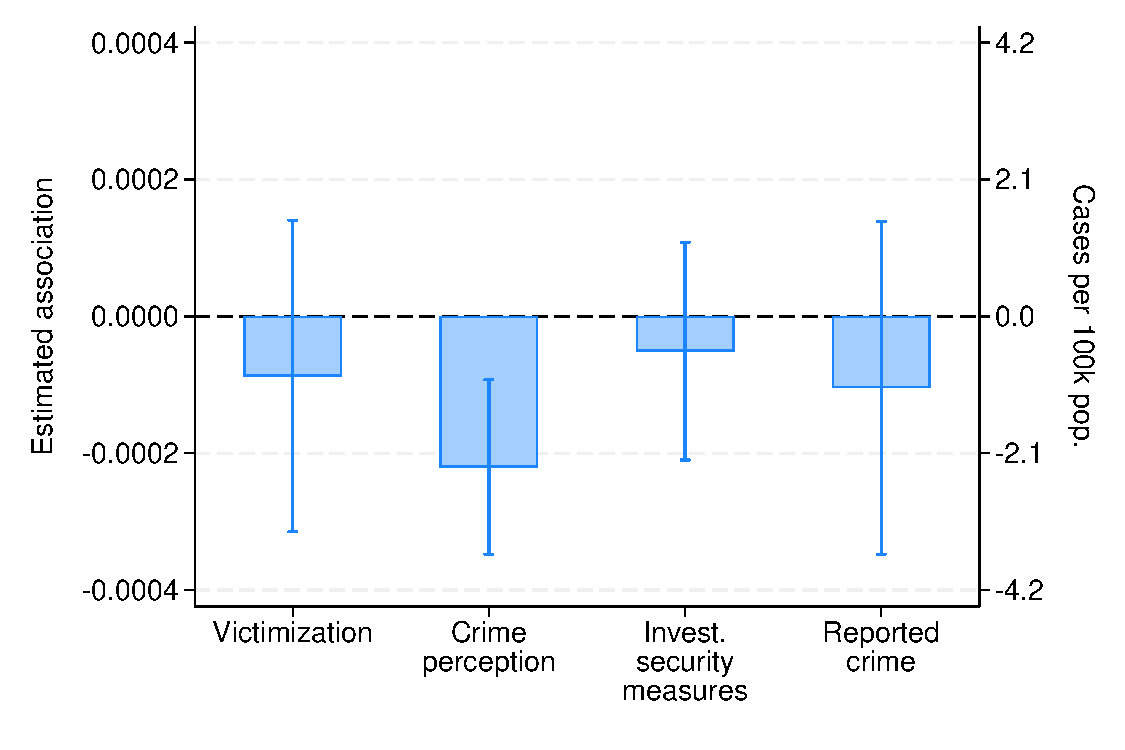
\includegraphics[width=\linewidth]{../manuscript/Graphs/results_corr_novariation_off_santiago.pdf}
        \caption{Association between police officers and effectiveness}
    \end{subfigure}
    \\[6pt]
    \begin{subfigure}[t]{0.55\textwidth}
        \centering
        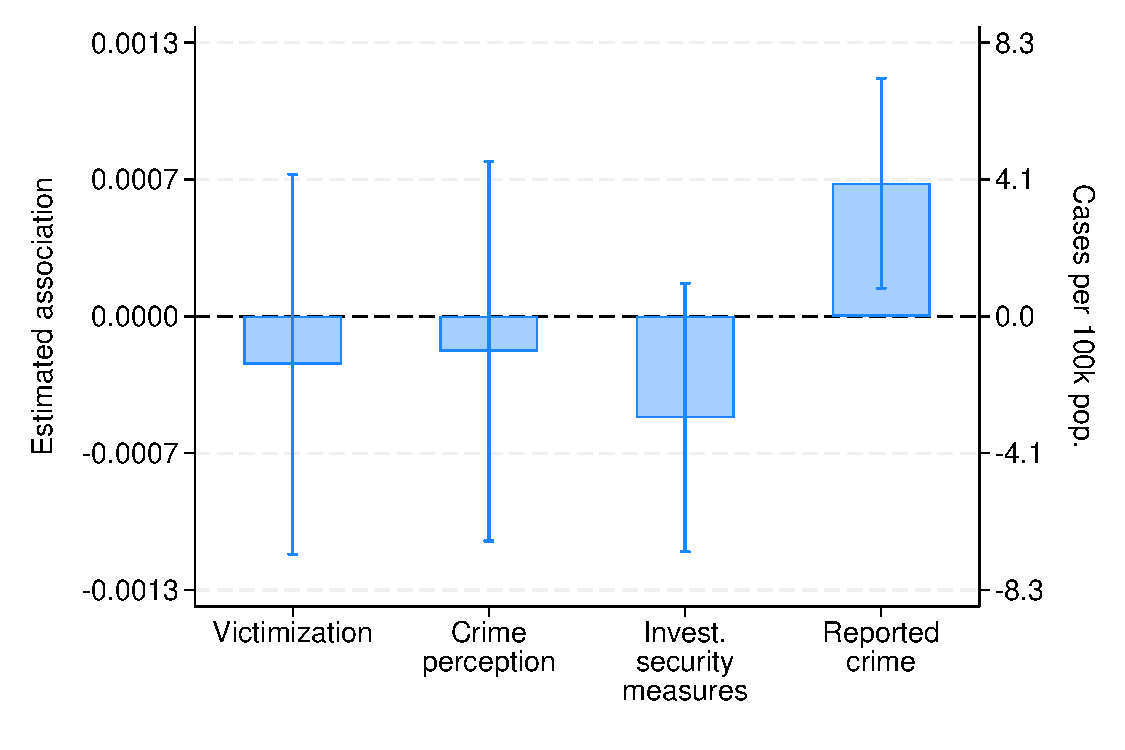
\includegraphics[width=\linewidth]{../manuscript/Graphs/results_corr_novariation_veh_santiago.pdf}
        \caption{Association between patrol vehicles and effectiveness}
    \end{subfigure}
    \\[8pt]
    \begin{minipage}{0.99\textwidth}
    \footnotesize Notes: Panel (a) reports the pooled effect of \emph{Seguridad Ciudadana}, a program that expanded local security personnel to support patrolling and deterrence but did not replicate the deployment-and-strategy features of \emph{Plan Cuadrante}. Panels (b) and (c) report within-municipality associations between police resources and police-effectiveness outcomes among the 41 municipalities of the Santiago Metropolitan Region, all of which had adopted \emph{Plan Cuadrante} by 2000. The regressions include municipality and year fixed effects. Standard errors are clustered at the municipality level using the wild bootstrapping procedure.
    \end{minipage}
\end{figure}
\FloatBarrier

To further investigate whether resource increases alone can explain our results, we assess the effects of \emph{Seguridad Ciudadana}, a program that expanded local security personnel to support patrolling and deterrence, but did not replicate the core deployment-and-strategy features of \emph{Plan Cuadrante}. Using a difference-in-differences specification following \citet{Callaway}, panel (a) of Figure \ref{fig:resources2} shows no significant effects of these resource changes on police effectiveness. Further details about this exercise and the corresponding event-study estimates are reported in Online Appendix \ref{sec:appendixB} and Online Appendix Figure \ref{fig:figureA5}. 


Finally, we study whether variation in police resources in municipalities that had already adopted \emph{Plan Cuadrante} improves public safety and security perceptions. Using ENUSC data and information on resources for 2006--2012 in the 41 municipalities of the Santiago Metropolitan Region---all of which had adopted \emph{Plan Cuadrante} by 2000---we exploit variation in officers and patrol vehicles that is unrelated to program adoption. Panels (b) and (c) of Figure \ref{fig:resources2} show the association between police resources and our main outcomes, conditional on municipality and year fixed effects. With one exception---the association between police officers and crime perception---none of these associations is statistically significant at conventional confidence levels. \footnote{Online Appendix Figure \ref{fig:figureA7B} reports the same exercise and also shows similar results for the broader set of municipalities that adopted \emph{Plan Cuadrante} before 2006 and never-treated municipalities (red bars); see Online Appendix \ref{sec:appendixB} for further details.}

Taken together, these results suggest that resource increases alone do not account for the effects of \emph{Plan Cuadrante}. We next turn to evidence that speaks more directly to the beat-policing components of the reform.

Panel (a) of Figure \ref{fig:police_performance} shows that, following the adoption of \emph{Plan Cuadrante}, households are much more likely to report increased police presence in their neighborhoods. The share of households perceiving increased police presence rises by 35 percentage points (156\%), the share reporting that police pass by their house daily rises by 22 percentage points (59\%), the share reporting never seeing police patrols near their house falls by 10 percentage points (57\%), and complaints about lack of police surveillance fall by around 5 percentage points (20\%). This evidence is consistent with both larger resources and the new deployment model. Yet the latter estimate---the only police-presence outcome for which we can separately estimate effects in municipalities with small and large resource increases---is similar in magnitude across the two groups, which suggests that the increase in police presence is not explained only by larger resource increases (see Online Appendix Figure \ref{fig:heterogeneity_appendix}).\footnote{We cannot estimate heterogeneous effects for other police-presence outcomes, such as the reporting of police passing by or the share of households perceiving an increase in police presence, because those variables are available only in ENUSC rounds 2003, 2005, and 2006, while resource data start in 2006.} More importantly, the broader pattern of results suggests that \emph{Plan Cuadrante} did more than simply increase patrolling intensity. Existing work shows that police presence can reduce crime while officers are present, but that its overall effects may be attenuated when crime is displaced across places or time windows \citep{MASTROBUONI2019, Blanes_Mastrobuoni_2018}. Our results point to something broader. As discussed in Section \ref{results}, we find actual declines in victimization and reported crime, together with no evidence of spillovers to neighboring municipalities. This pattern is more consistent with officers accumulating local knowledge and adapting prevention strategies to local conditions under stable territorial assignment than with a purely mechanical increase in patrol intensity.

Panel (b) of Figure \ref{fig:police_performance} reinforces this interpretation. Households in early-adopting municipalities report better police performance across multiple dimensions. They are 8.1 percentage points (16\%) more likely to rate police performance as good or very good, 7.6 percentage points (11\%) more likely to describe police as efficient, 5 percentage points (6\%) more likely to report that police are helpful, and 4.9 percentage points (7\%) more likely to report that police are well informed. They are also 3.9 percentage points (10\%) less likely to perceive police as corrupt, 7.9 percentage points (21\%) less likely to believe police fail to control crime, and 7.6 percentage points (22\%) less likely to report that police do not perform their duties effectively.\footnote{Information on police performance is only available in ENUSC round 2005. Using this round, we compare perceived police performance in municipalities that adopted \emph{Plan Cuadrante} in 2005 or earlier and in municipalities adopting after 2005. Figure \ref{fig:balance_doseresponse} in Online Appendix \ref{sec:appendixB} shows that the number of years of exposure to \emph{Plan Cuadrante} is positively correlated with perceived police performance. While these exercises on perceived police performance should be interpreted with caution, we show in the same appendix that the timing of future adoption is not correlated with perceived police performance in 2005 for municipalities that had not yet adopted the program by 2005.} %These perceived improvements are consistent with a setting in which officers become better informed about local routines and more effective in how they patrol and respond.

The administrative evidence points in the same direction. Panel (c) of Figure \ref{fig:police_performance} shows that arrests per 100,000 inhabitants increase by 48 (14\%) in our main estimates, even as crime declines overall.\footnote{As with reported crime, this event study is restricted to 5 pre-treatment and 7 post-treatment periods for symmetry with the ENUSC-based analysis; Online Appendix Figure \ref{fig:admin_uncapped} reports the results for arrests using the full set of pre-treatment and post-treatment periods.} This effect is also significant among municipalities with resource increases similar to those in the control group (see Online Appendix Figure \ref{fig:heterogeneity_appendix}). Consistent with this pattern, panel (d) of Figure \ref{fig:police_performance} shows that the arrest rate per reported crime also increases by 1.7 percentage points (10\%), suggesting that a higher share of crimes reported to the police are being solved. Because these gains appear even where resources did not increase more than in control municipalities, they are difficult to reconcile with a pure resource story and are more naturally interpreted as improvements in police effectiveness under the deployment and strategy changes introduced by \emph{Plan Cuadrante}. The corresponding event-study estimates for arrests, the arrest rate per reported crime, and trust in the police in Figure \ref{fig:police_performance} confirm that these changes emerge only after adoption.

Finally, panel (e) of Figure \ref{fig:police_performance} shows a sharp increase in trust in the police in our main specification (Section \ref{results}), consistent with one of the objectives of beat policing, namely bringing officers closer to the community and allowing them to accumulate local knowledge through repeated interaction. Online Appendix Figure \ref{fig:heterogeneity_appendix} shows that this effect remains sizeable both in municipalities that experienced resource increases similar to the control group and in those with larger increases.

Overall, although resources were likely important for implementation and may explain part of the effects in some municipalities, the results in this section indicate that resource changes alone are not enough to explain our findings. The evidence is more consistent with a combination of deployment changes and the strategy adjustments enabled by local knowledge accumulation under permanent assignment to quadrants.

\FloatBarrier
%--- Implementation
\begin{figure}[!ht]
    \centering
    \caption[\emph{Plan Cuadrante} and Changes in Police Performance]{\emph{Plan Cuadrante} and Changes in Police Performance}
    \label{fig:figure05}
    \label{fig:police_performance}
    \label{fig:effectiveness_es}
    \begin{subfigure}[t]{0.44\textwidth}
        \centering
        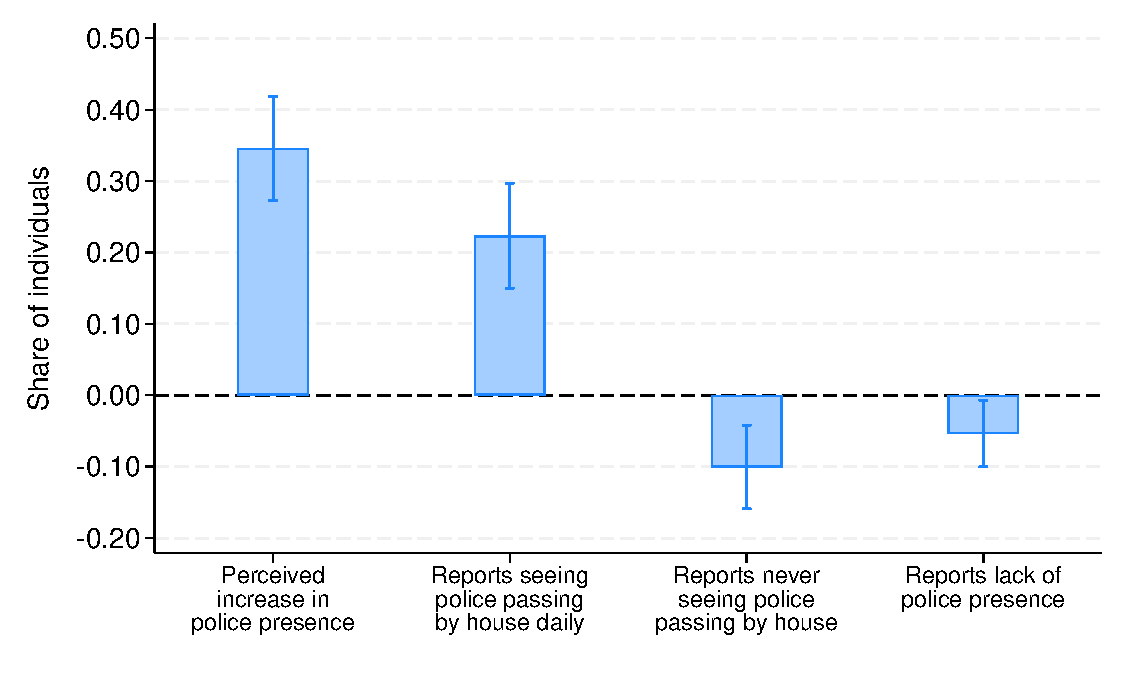
\includegraphics[width=\linewidth]{../manuscript/Graphs/results_policepresence.pdf}
        \caption{Effect on police presence}
    \end{subfigure}\hfill
    \begin{subfigure}[t]{0.44\textwidth}
        \centering
        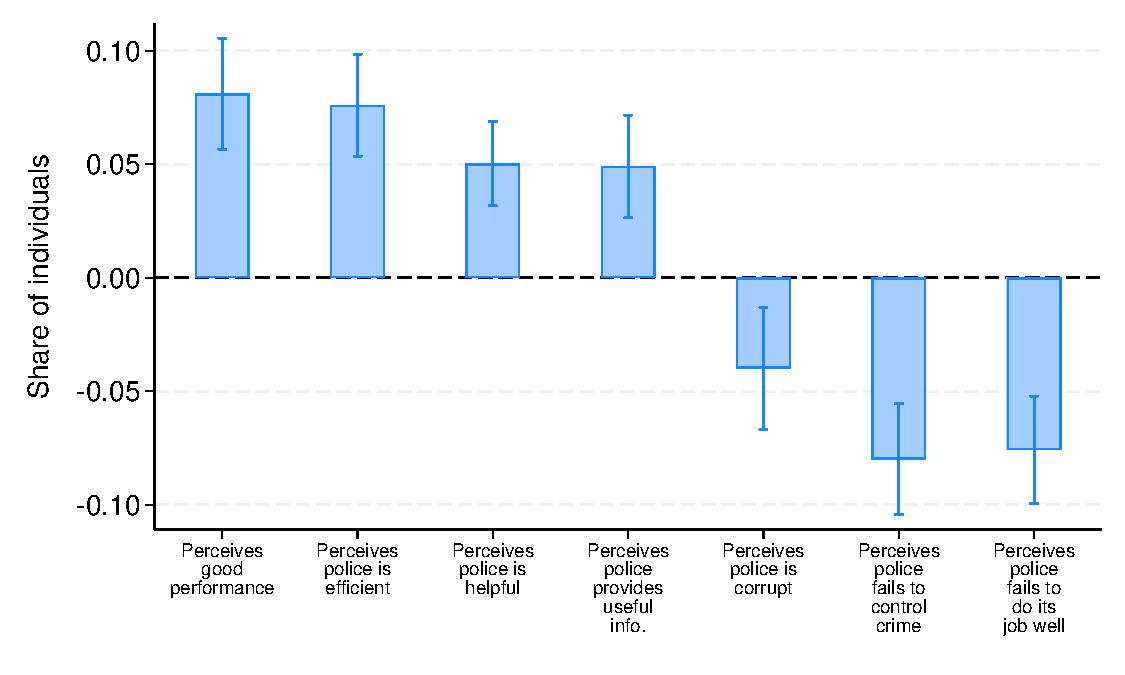
\includegraphics[width=\linewidth]{../manuscript/Graphs/combined_PCttest_2.pdf}
        \caption{Effect on perceived police performance}
    \end{subfigure}
    \\[6pt]
    \begin{subfigure}[t]{0.44\textwidth}
        \centering
        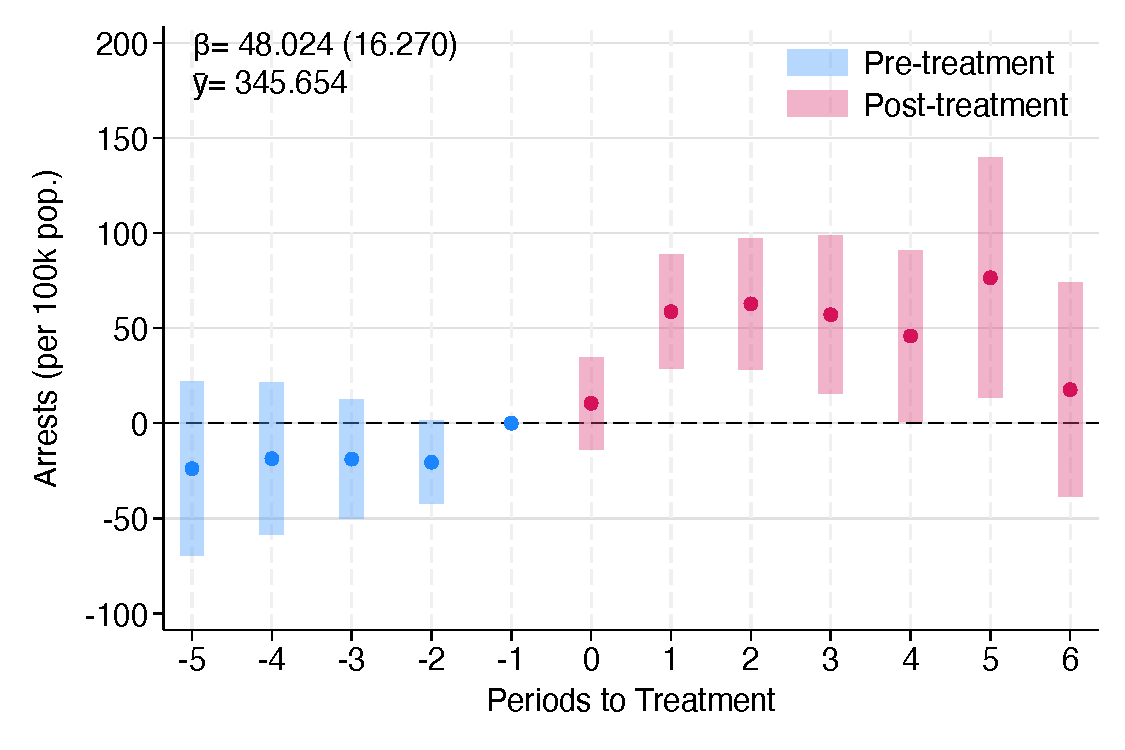
\includegraphics[width=\linewidth]{../manuscript/Graphs/totalarrestscrime_allcomunas.pdf}
        \caption{Arrests (per 100k pop.)}
    \end{subfigure}\hfill
    \begin{subfigure}[t]{0.44\textwidth}
        \centering
        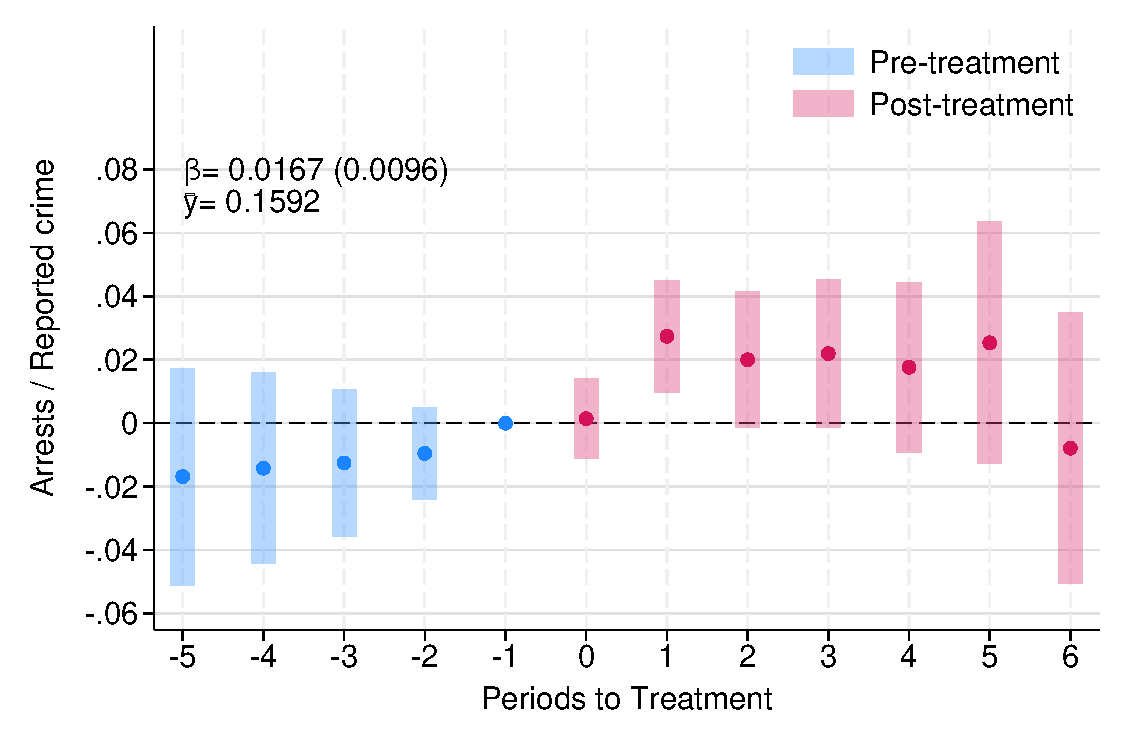
\includegraphics[width=\linewidth]{../manuscript/Graphs/arrests_over_reportedcrime_allcomunas.pdf}
        \caption{Arrests / Reported crime}
    \end{subfigure}
    \\[6pt]
    \begin{subfigure}[t]{0.44\textwidth}
        \centering
        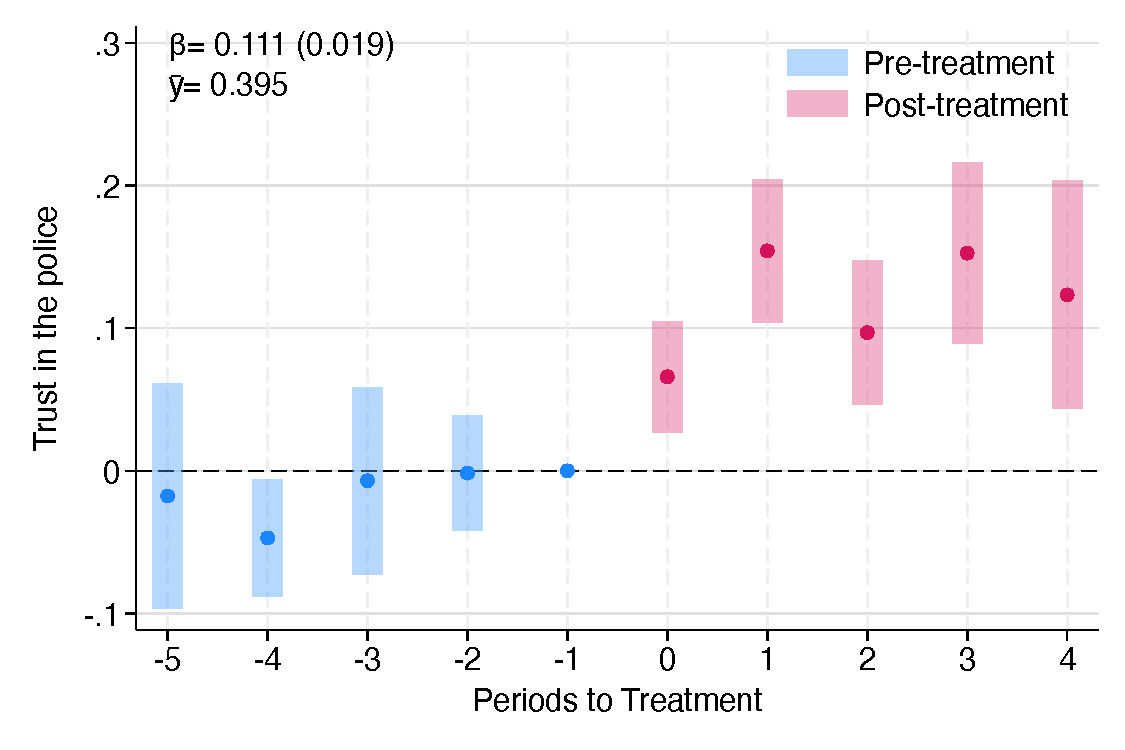
\includegraphics[width=\linewidth]{../manuscript/Graphs/results_trustcarabineros.pdf}
        \caption{Trust in the police}
    \end{subfigure}
    \\[8pt]
    \begin{minipage}{0.99\textwidth}
    \footnotesize Notes: Panel (a) reports the effects on perceived police presence. Panel (b) reports perceived police performance in 2005, comparing municipalities where \emph{Plan Cuadrante} was already implemented before 2006 with municipalities where it was implemented after 2005. Panels (c), (d), and (e) report dynamic event-study estimates for arrests per 100,000 inhabitants, the ratio of arrests to reported crime, and trust in the police. The estimation follows \citet{Callaway}. The graphs display estimated coefficients and 95\% confidence intervals. Standard errors are clustered at the municipality level using the wild bootstrapping procedure.
    \end{minipage}
\end{figure}

\FloatBarrier

%Overall, while resources were arguably important for implementation, the evidence suggests that the beat policing elements---permanent assignment of officers to quadrants and greater local knowledge---were important drivers of the improvements in public safety and security perceptions we document in the paper.



 
}
\end{adjustwidth}

\clearpage
\noindent\textbf{Other figures and tables referenced above:}
\vspace{0.5em}

{\setcounter{figure}{1}\renewcommand{\thefigure}{\arabic{figure}}
%--- Implementation
\begin{figure}[h!]
    \centering
    \caption{Effects of \emph{Plan Cuadrante} on Crime Outcomes and Security Perceptions}
    \label{fig:figure02}
    \begin{subfigure}{0.495\textwidth}
        \centering
        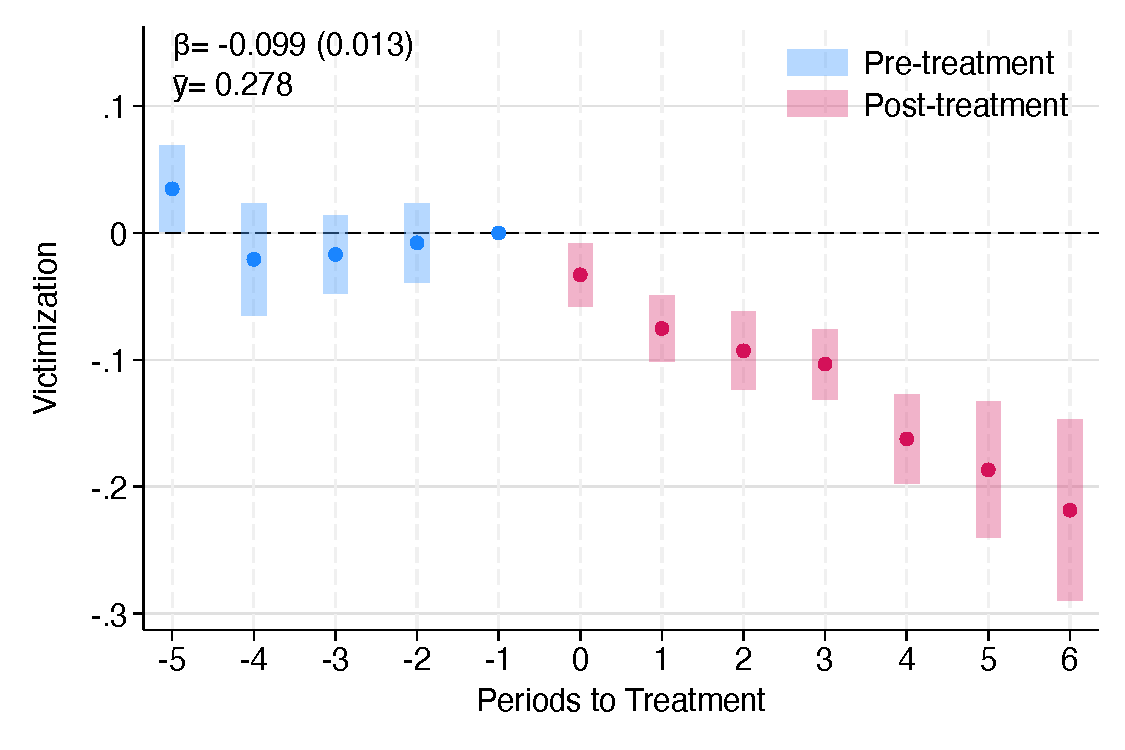
\includegraphics[width=\textwidth]{../manuscript/Graphs/results_victimization.pdf}
        \caption{Victimization in last 12 months}
    \end{subfigure}%
    ~
    \begin{subfigure}{0.495\textwidth}
    \centering
    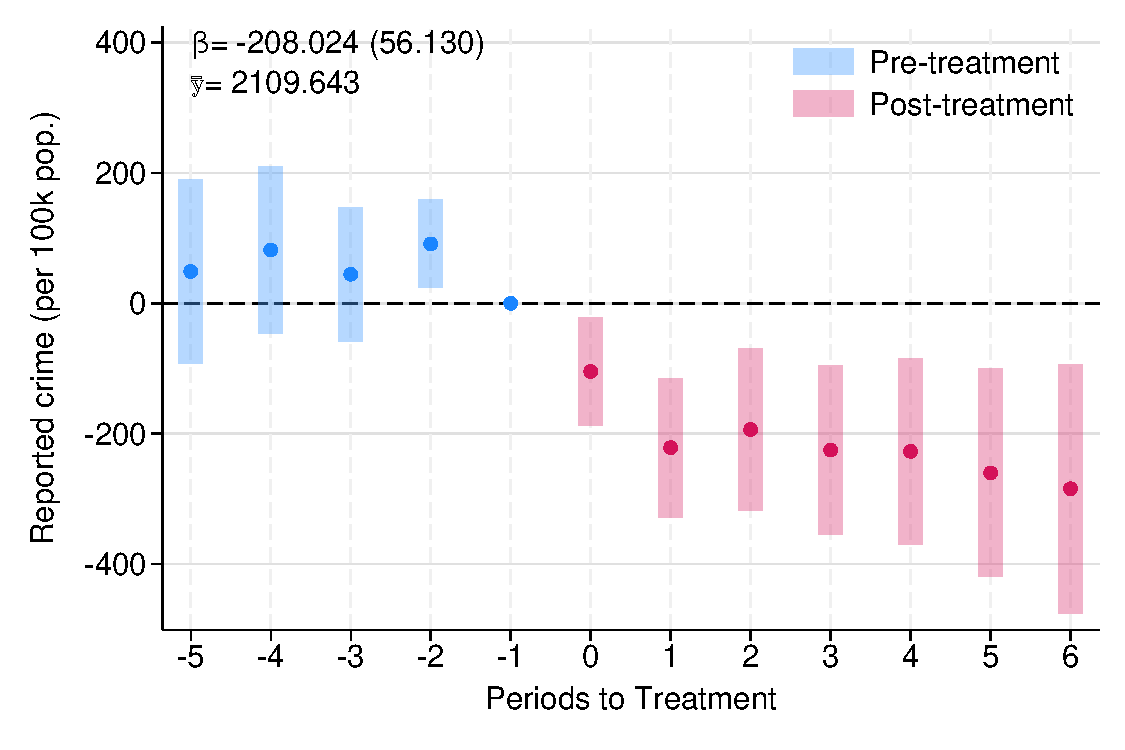
\includegraphics[width=\textwidth]{../manuscript/Graphs/totalreportedcrime_allcomunas.pdf}
        \caption{Reported crime per 100k inhabitants}
    \end{subfigure}
        \begin{subfigure}{0.495\textwidth}
        \centering
        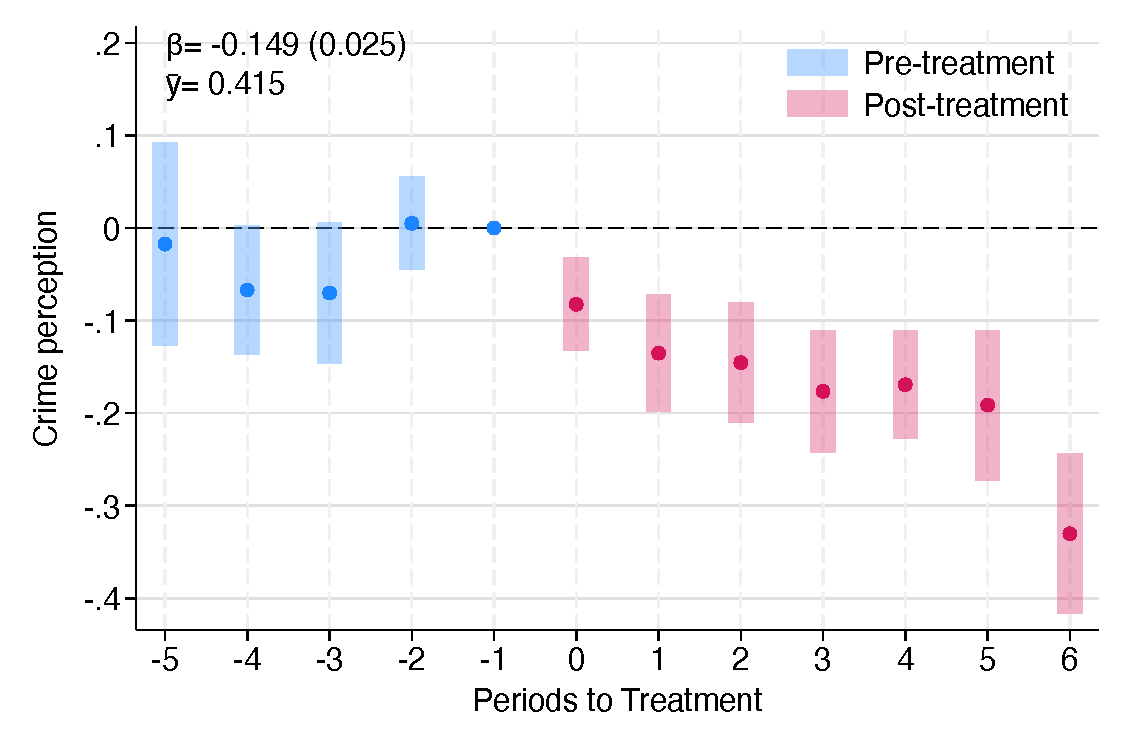
\includegraphics[width=\textwidth]{../manuscript/Graphs/results_perception.pdf}
        \caption{Households reporting an increase in crime}
    \end{subfigure}%
    ~
    \begin{subfigure}{0.495\textwidth}
    \centering
    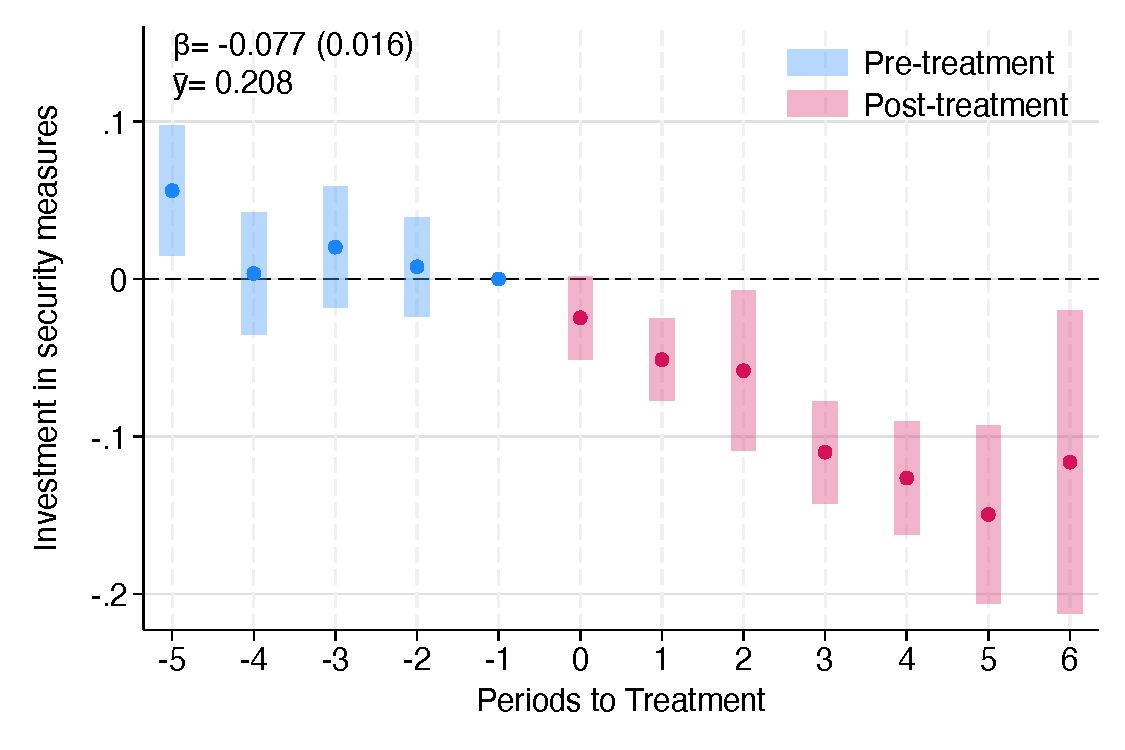
\includegraphics[width=\textwidth]{../manuscript/Graphs/results_hhprotectionmeasures.pdf}
        \caption{Households adopting security measures}
    \end{subfigure}
    \\[12pt]
    \begin{minipage}{0.99\textwidth}
    \footnotesize
    Notes: This figure shows the dynamic effects of the \emph{Plan Cuadrante} on different measures of police effectiveness. The estimation is conducted using the procedure developed in \citet{Callaway} for difference-in-differences with staggered treatment adoption. The dots in the figure represent the estimated coefficients and the bars behind them 95\% confidence intervals. Standard errors are clustered at the municipality level using the wild bootstrapping procedure. The pooled effect and the mean outcome before the introduction of the treatment is also presented in each panel. Panel (a) reports the effect of \emph{Plan Cuadrante} on the probability of household victimization in the last 12 months using the ENUSC survey. Panel (b) reports the effect on the number of crimes reported to the police in the municipality per 100,000 inhabitants using administrative data. Panel (c) reports the effect on the probability of perceiving an increase in crime using the ENUSC survey. Panel (d) reports the effect on the probability of adopting security measures in the last twelve months using the ENUSC survey. Panel (a) includes 93,041 observations; panel (b), 4,231; panel (c), 89,578; and panel (d), 93,041 observations.
    \end{minipage}
\end{figure}
}

\clearpage

{\renewcommand{\thetable}{B.3}
\begin{table}[h!]\centering
\caption{Effects of \emph{Plan Cuadrante} Controlling for Police Resources}
\label{tab:results_controlbyresources}
\resizebox{\textwidth}{!}{
\begin{threeparttable}
\begin{tabular}{l ccccc}
\toprule
 & (1) & (2) & (3) & (4) & (5) \\
\midrule
\multicolumn{6}{l}{\textit{Panel A. Victimization}} \\[0.2em]
ATT &       -0.099*** &       -0.077*** &       -0.086** &       -0.094*** &       -0.087* \\
  & (0.013) & (0.013) & (0.043) & (0.028) & (0.053) \\
N &    93,041 &    53,973 &    53,553 &    72,017 &    53,553 \\[0.4em]
\multicolumn{6}{l}{\textit{Panel B. Crime perception}} \\[0.2em]
ATT &       -0.149*** &       -0.140*** &       -0.112** &       -0.082** &       -0.111 \\
  & (0.025) & (0.032) & (0.057) & (0.033) & (0.106) \\
N &    89,578 &    52,160 &    51,746 &    69,434 &    51,746 \\[0.4em]
\multicolumn{6}{l}{\textit{Panel C. Investment in security measures}} \\[0.2em]
ATT &       -0.077*** &       -0.066*** &       -0.109*** &       -0.081*** &       -0.168*** \\
  & (0.016) & (0.019) & (0.041) & (0.019) & (0.064) \\
N &    93,041 &    53,973 &    53,553 &    72,017 &    53,553 \\[0.4em]
\multicolumn{6}{l}{\textit{Panel D. Reported crime (per 100k pop.)}} \\[0.2em]
ATT &     -208.024*** &     -190.446*** &       29.230 &     -261.439 &     -245.555 \\
  & (56.130) & (67.908) & (147.261) & (170.954) & (165.221) \\
N &     4,231 &     1,918 &     1,911 &     2,248 &     1,911 \\[0.4em]
\midrule
Sample                   & Full & Resource yrs & Resource yrs & Resource yrs & Resource yrs \\
Police officers (per 100k pop.) &      &            & \checkmark &            & \checkmark \\
Patrol vehicles (per 100k pop.) &      &            &            & \checkmark & \checkmark \\
\bottomrule
\end{tabular}
\begin{tablenotes}[flushleft]
\item \footnotesize{Note: ATT estimates of the effect of \emph{Plan Cuadrante} on each outcome. Column (1) is the baseline (full estimation sample, no controls) and reproduces the headline estimate of the corresponding estimator. Column (2) restricts the estimation to 2006--2012, the window over which police resources are observed, without including any control variable. Columns (3)--(5) add time-varying controls for police resources per 100{,}000 inhabitants: officers only; patrol vehicles only; and officers and patrol vehicles jointly (entered as separate regressors). Columns (3) and (5) cover 2006--2012, the years for which the number of officers is observed; column (4) also includes 2005, the first year for which patrol vehicles are observed. Patrol vehicles are measured, per 100{,}000 inhabitants, as all patrol automobiles (radiopatrulla, auto patrullero, auto policial, automovil, station wagon, jeep and camioneta) plus motorcycles. Standard errors in parentheses; row N reports the estimation-sample size. Estimation follows \citet{Callaway}; standard errors clustered at the municipality level using wild bootstrapping procedures. $^{*}p<0.1$, $^{**}p<0.05$, $^{***}p<0.01$.}
\end{tablenotes}
\end{threeparttable}}
\end{table}
}

\clearpage

{\renewcommand{\thefigure}{B.3}
\begin{figure}[h!]
    \centering
    \caption{Effects of \emph{Plan Cuadrante} by Resource Increase: Trust, Complaints, and Arrests}
    \label{fig:heterogeneity_appendix}
    \begin{subfigure}[t]{0.48\textwidth}
        \centering
        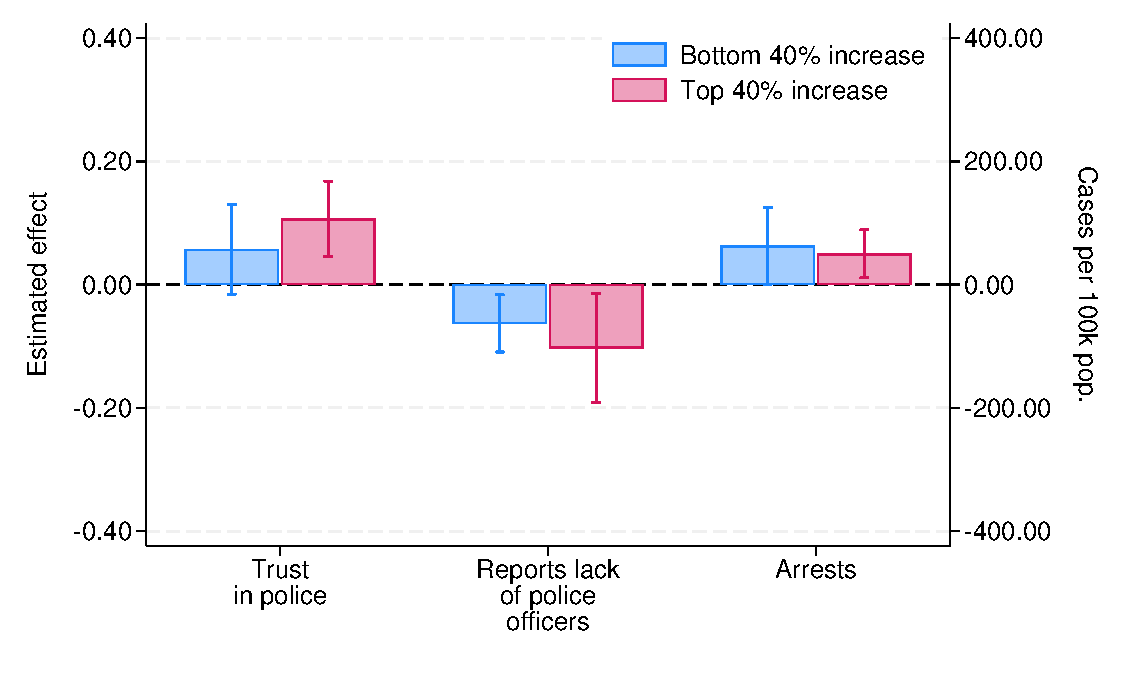
\includegraphics[width=\linewidth]{../manuscript/Graphs/heterogeneity_off_appendix.pdf}
        \caption{By the intensity of $\Delta$ in police officers}
    \end{subfigure}\hfill
    \begin{subfigure}[t]{0.48\textwidth}
        \centering
        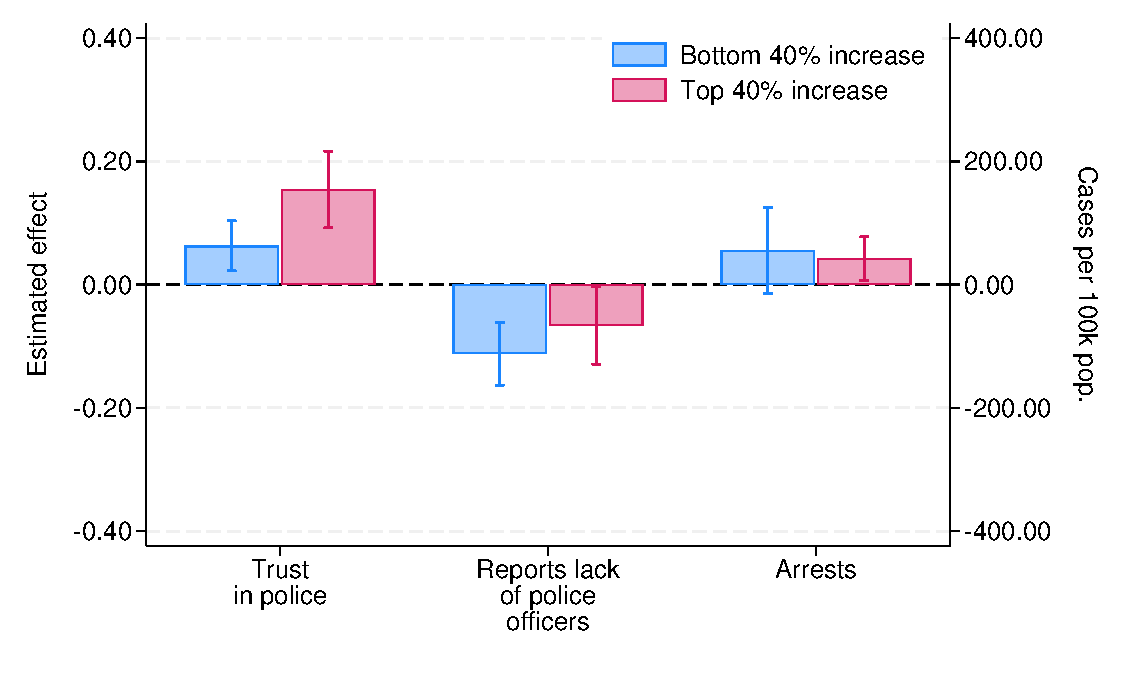
\includegraphics[width=\linewidth]{../manuscript/Graphs/heterogeneity_pv_appendix.pdf}
        \caption{By the intensity of $\Delta$ in patrol vehicles}
    \end{subfigure}
    \\[8pt]
    \begin{minipage}{0.99\textwidth}
    \footnotesize Notes: This figure complements Figure \ref{fig:figure_resources} by reporting, for the three outcomes not shown there, the effect of \emph{Plan Cuadrante} estimated separately for municipalities in the bottom 40\% (blue) and top 40\% (red) of the resource-increase distribution. Panel (a) splits municipalities by the increase in police officers and panel (b) by the increase in patrol vehicles. In each panel, arrests (administrative data, in cases per 100,000 inhabitants) are read on the right axis; the other two outcomes, from the ENUSC survey (trust in the police, and reports about the lack of police officers), are read on the left axis. Effects are estimated using the difference-in-differences estimator for staggered treatment adoption developed in \citet{Callaway}; bars are point estimates and whiskers 95\% confidence intervals, with standard errors clustered at the municipality level using the wild bootstrapping procedure.
    \end{minipage}
\end{figure}
}

\clearpage

{\renewcommand{\thefigure}{B.4}
\begin{figure}[h!]
    \centering
    \caption{Effects of \textit{Seguridad Ciudadana} on Crime Outcomes and Security Perceptions}
    \label{fig:figureA5}
    
    % Primera fila: panel (a) y (b)
    \begin{subfigure}{0.495\textwidth}
        \centering
        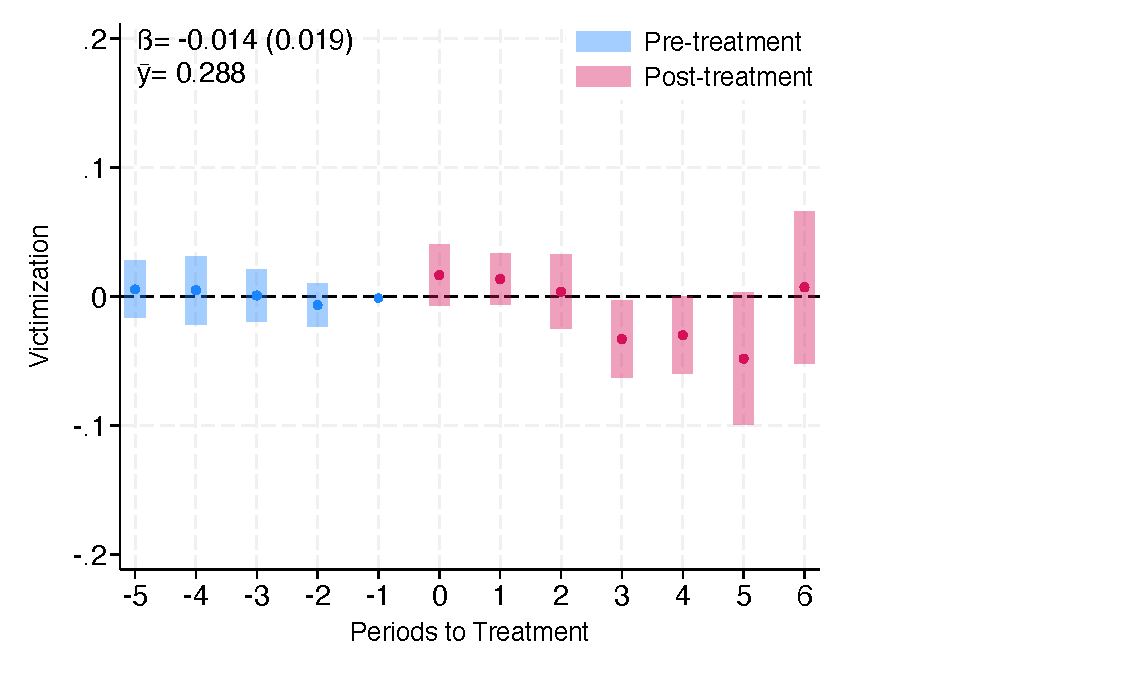
\includegraphics[width=\textwidth]{../manuscript/Graphs/results_victimization_SC.pdf}
        \caption{Victimization in last 12 months}
    \end{subfigure}%
    \hfill
    \begin{subfigure}{0.495\textwidth}
        \centering
        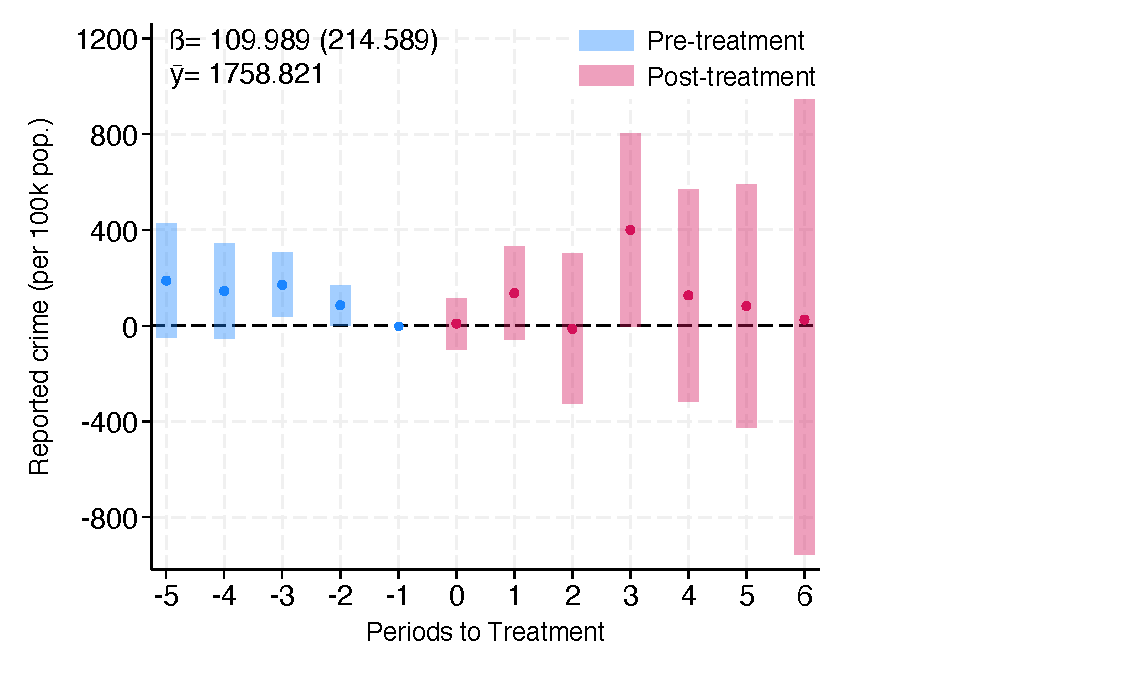
\includegraphics[width=\textwidth]{../manuscript/Graphs/totalreportedcrime_allcomunas_SC.pdf}
        \caption{Reported crime per 100k inhabitants}
    \end{subfigure}

    \vspace{12pt} % Espacio entre filas
    
    % Segunda fila: panel (c) y (d)
    \begin{subfigure}{0.495\textwidth}
        \centering
        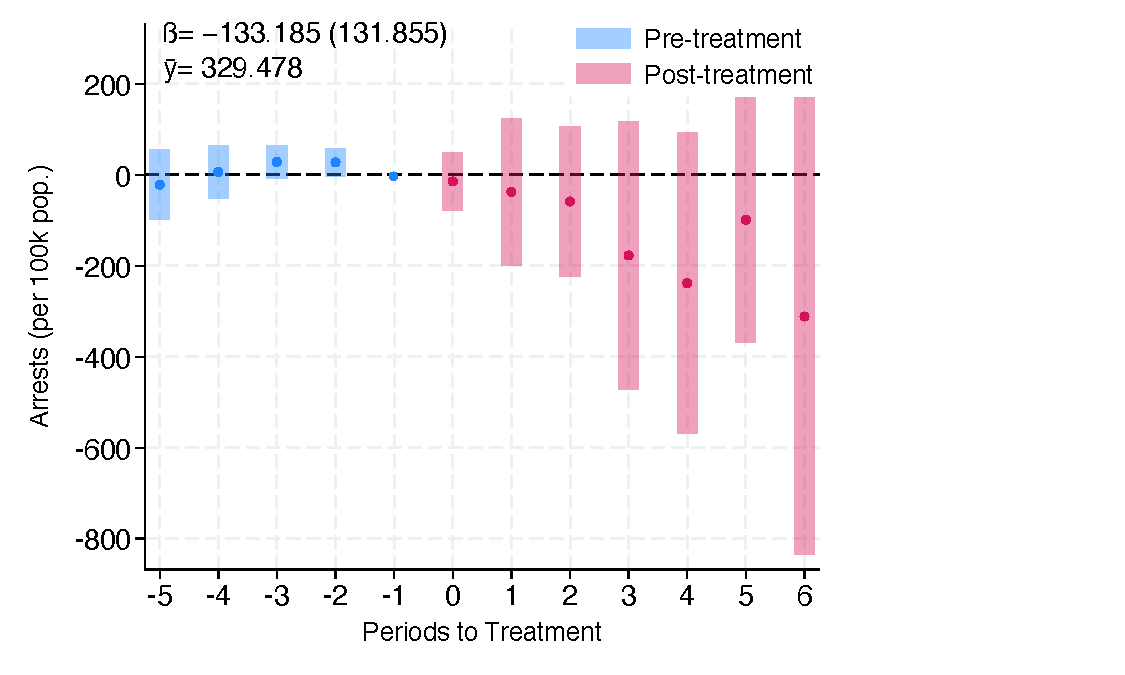
\includegraphics[width=\textwidth]{../manuscript/Graphs/totalarrestscrime_allcomunas_SC.pdf}
        \caption{Arrests per 100k inhabitants}
    \end{subfigure}%
    \hfill
    \begin{subfigure}{0.495\textwidth}
        \centering
        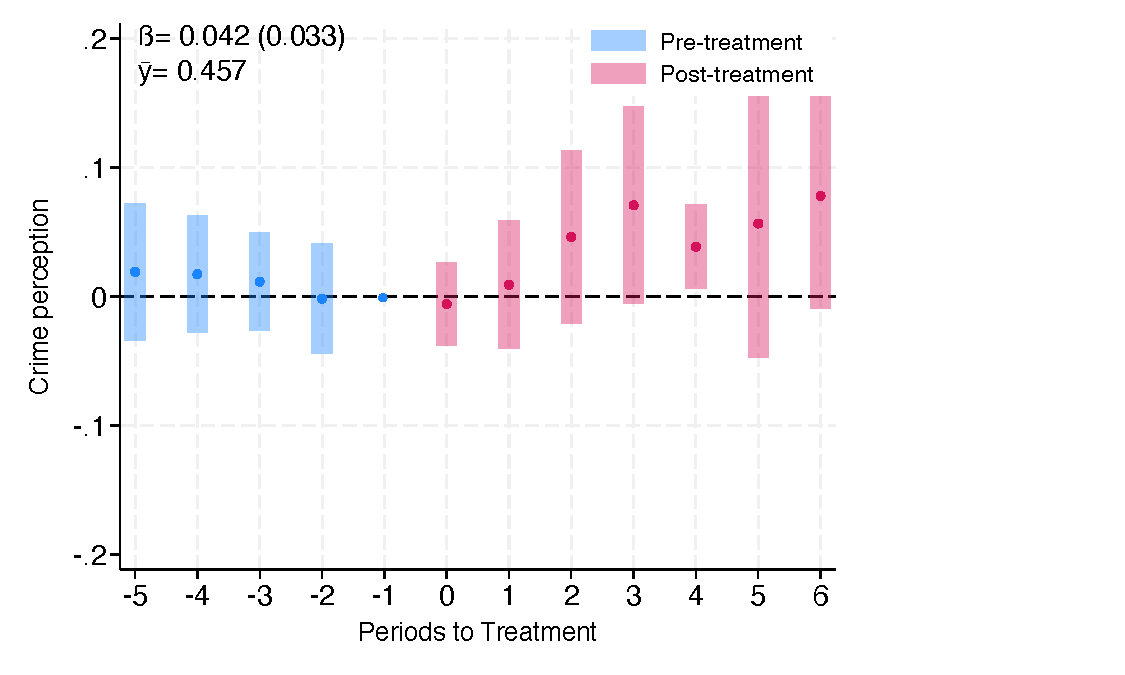
\includegraphics[width=\textwidth]{../manuscript/Graphs/results_perception_SC.pdf}
        \caption{Households reporting an \\ increase in crime}
    \end{subfigure}
    
    \vspace{12pt} % Espacio entre filas
    
    % Tercera fila: panel (e)
    \begin{subfigure}{0.495\textwidth}
        \centering
        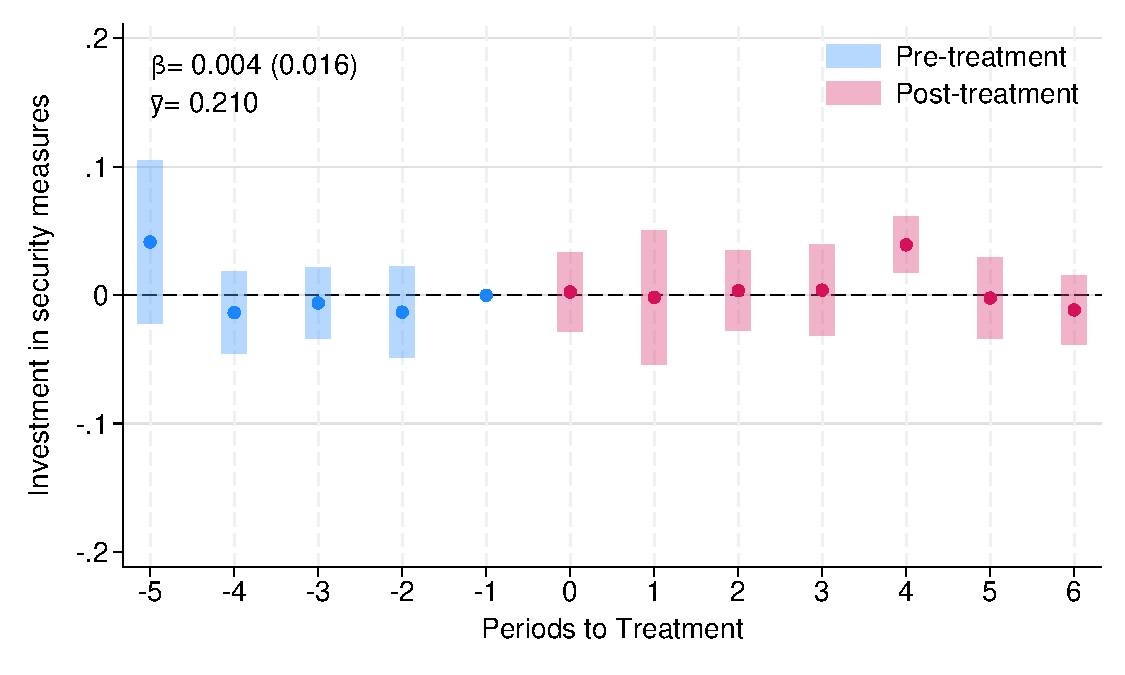
\includegraphics[width=\textwidth]{../manuscript/Graphs/results_hhprotectionmeasures_SC.pdf}
        \caption{Households adopting security measures}
    \end{subfigure}

    \vspace{12pt} % Espacio para las notas
    
    \begin{minipage}{0.99\textwidth}
        \footnotesize
        Notes: This figure shows the dynamic effects of the \textit{Seguridad Ciudadana} program on different measures of crime and security perceptions. The estimation is conducted using the procedure developed in \citet{Callaway} for difference-in-differences with staggered treatment adoption. The dots in the figure represent the estimated coefficients and the bars behind them 95\% confidence intervals. Standard errors are clustered at the municipality level using wild bootstrapping. The pooled effect and the mean outcome before the introduction of the treatment for the outcome---computed as in Figure \ref{fig:figure02}, using only the pre-treatment observations of treated units---is also presented in each panel. Panel (a) reports the effect of \textit{Seguridad Ciudadana} on the probability of household victimization in the last 12 months using the ENUSC survey. Panel (b) reports the effect on the number of crimes reported to the police in the municipality per 100,000 inhabitants using administrative data. Panel (c) reports the effect on the number of arrests in the municipality per 100,000 inhabitants using administrative data. Panel (d) reports the effect on the probability of perceiving an increase in crime using the ENUSC survey. Panel (e) reports the effect on the probability of adopting security measures in the last twelve months using the ENUSC survey. Panel (a) includes 210,102 observations; panel (b), 2,234; panel (c), 1,908; panel (d), 203,078; and panel (e), 74,316 observations.
    \end{minipage}
\end{figure}
}

\clearpage

{\renewcommand{\thefigure}{B.5}
\begin{figure}[h!]
    \centering
    \caption{Association between Police Resources and Police Effectiveness (No \emph{Plan Cuadrante} Variation)}
    \label{fig:figureA7B}
    \begin{subfigure}[t]{0.48\textwidth}
        \centering
        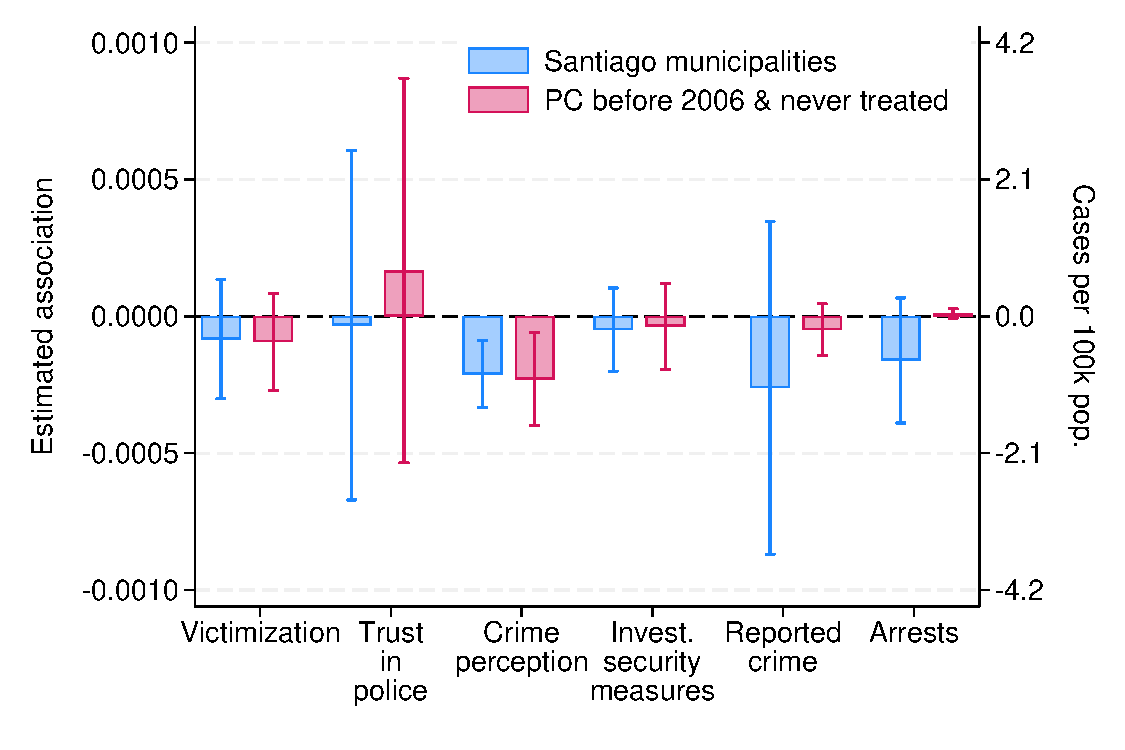
\includegraphics[width=\linewidth]{../manuscript/Graphs/results_corr_novariation_off.pdf}
        \caption{Association with police officers}
    \end{subfigure}\hfill
    \begin{subfigure}[t]{0.48\textwidth}
        \centering
        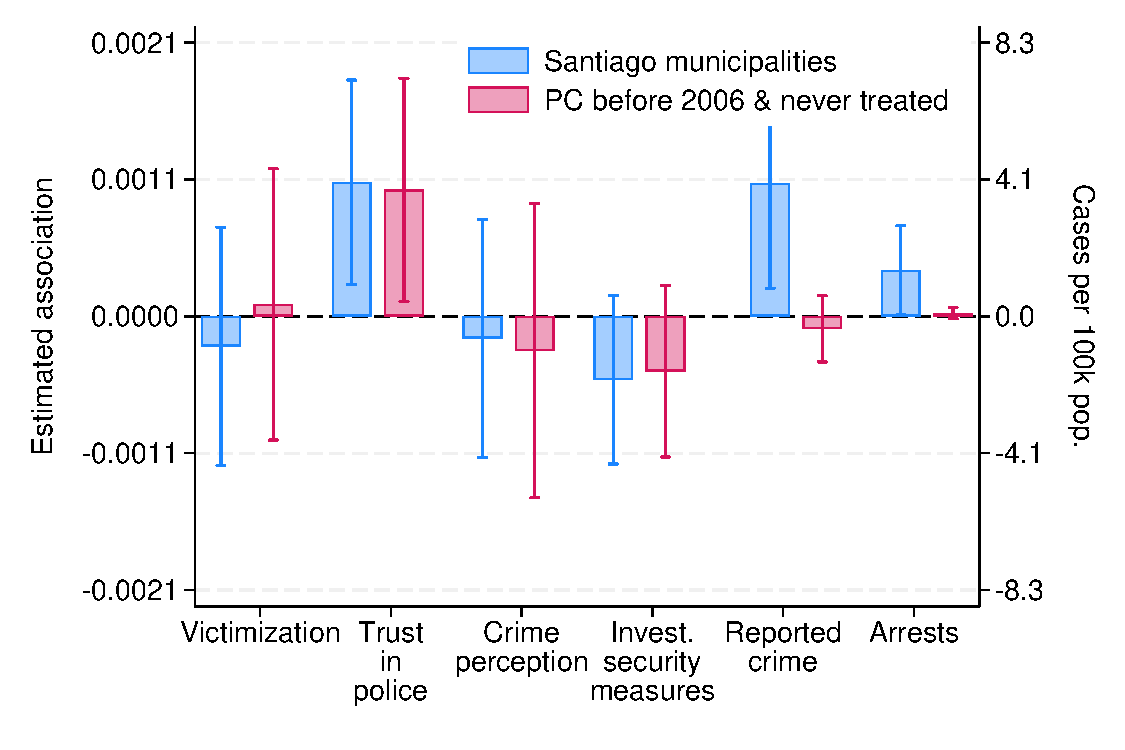
\includegraphics[width=\linewidth]{../manuscript/Graphs/results_corr_novariation_veh.pdf}
        \caption{Association with patrol vehicles}
    \end{subfigure}
    \\[10pt]
    \begin{minipage}{0.99\textwidth}
    \footnotesize Notes: The figure shows the estimated within-municipality association between police resources (per 100,000 inhabitants) and the main outcomes, in municipalities where \emph{Plan Cuadrante} does not vary over the sample period. Estimates come from OLS regressions of each outcome on the resource measure with municipality and year fixed effects; standard errors are clustered at the municipality level. Blue bars use the 41 metropolitan municipalities of Santiago, all of which adopted \emph{Plan Cuadrante} in 2000; red bars use the broader set of municipalities that adopted \emph{Plan Cuadrante} before 2006 together with the never-treated municipalities surveyed in ENUSC (2006--2012). Reported crime and arrests (administrative data, in cases per 100,000 inhabitants) are read on the right axis; all other outcomes, from the ENUSC survey (victimization, trust in the police, crime perception, and investment in security measures), are read on the left axis. Panel (a) reports associations with the number of police officers; panel (b) with the number of patrol vehicles. Bars are point estimates with 95\% confidence intervals.
    \end{minipage}
\end{figure}
}

\clearpage

{\renewcommand{\thetable}{B.4}
\begin{table}[H]
\centering
\caption{Predictors of the Increase in Police Resources under \emph{Plan Cuadrante}}
\label{tab:resourcecorrelates}
\begin{threeparttable}
\small
\setlength{\tabcolsep}{6pt}
\renewcommand{\arraystretch}{1.1}
\begin{tabular}{@{}l cc cc@{}}
\toprule
& \multicolumn{2}{c}{Administrative sample} & \multicolumn{2}{c}{ENUSC sample} \\
\cmidrule(lr){2-3} \cmidrule(lr){4-5}
& Police & Patrol & Police & Patrol \\
Dep.\ var: avg.\ annual increase & officers & vehicles & officers & vehicles \\
in resources (share of pre-adoption level) & (1) & (2) & (3) & (4) \\
\midrule
Reported crime (per 100k pop.) & $-0.203^{**}$ & $-0.199^{**}$ & $-0.319^{*}$ & $0.272^{*}$ \\
 & (0.099) & (0.097) & (0.182) & (0.137) \\
Arrests (per 100k pop.) & $0.099$ & $-0.041$ & $0.003$ & $0.297$ \\
 & (0.136) & (0.129) & (0.186) & (0.223) \\
Victimization &  &  & $-0.017^{*}$ & $-0.025^{*}$ \\
 &  &  & (0.010) & (0.013) \\
Crime perception &  &  & $0.005$ & $0.008$ \\
 &  &  & (0.017) & (0.014) \\
Trust in the police &  &  & $0.024$ & $0.027$ \\
 &  &  & (0.018) & (0.019) \\
Investment in security measures &  &  & $0.004$ & $-0.003$ \\
 &  &  & (0.010) & (0.009) \\
Police officers (per 100k pop.) & $-0.207$ & $0.155$ & $-0.888^{***}$ & $0.571^{***}$ \\
 & (0.155) & (0.129) & (0.154) & (0.136) \\
Patrol vehicles (per 100k pop.) & $-0.129$ & $-0.139$ & $0.537^{**}$ & $-0.507^{***}$ \\
 & (0.129) & (0.126) & (0.212) & (0.169) \\
Log population & $-0.529^{***}$ & $-0.203^{*}$ & $-0.193$ & $-0.626^{**}$ \\
 & (0.145) & (0.112) & (0.189) & (0.269) \\
Poverty rate (2004) & $0.170$ & $0.308^{**}$ & $0.027$ & $-0.017$ \\
 & (0.113) & (0.126) & (0.108) & (0.108) \\
\midrule
Observations & 65 & 65 & 8,781 & 8,781 \\
R-squared & 0.342 & 0.282 & 0.614 & 0.545 \\
\bottomrule
\end{tabular}
\begin{tablenotes}[flushleft]
\footnotesize
\item \textit{Note:} OLS regressions of the average annual increase in police officers (columns 1 and 3) and patrol vehicles (columns 2 and 4) per 100{,}000 inhabitants, from the year before adoption of \emph{Plan Cuadrante} to 2012. As in panels (a) and (b) of Figure \ref{fig:figure_resources}, the increase is expressed as a share of the resources available the year before adoption. Columns 1--2 use the administrative sample at the municipality level; columns 3--4 use ENUSC survey respondents interviewed before 2007 (survey outcomes at the respondent level, other regressors as pre-2006 municipality aggregates). All variables are standardized. Standard errors clustered by municipality in parentheses.
\item $^{*}p<0.1$; $^{**}p<0.05$; $^{***}p<0.01$.
\end{tablenotes}
\end{threeparttable}
\end{table}
}

\clearpage

{\renewcommand{\thefigure}{B.6}
\begin{figure}[H]
    \centering
    \caption{Timing of Adoption of \emph{Plan Cuadrante} and Perceived Police Performance}
    \label{fig:balance_doseresponse}
    \begin{subfigure}{0.495\textwidth}
        \centering
        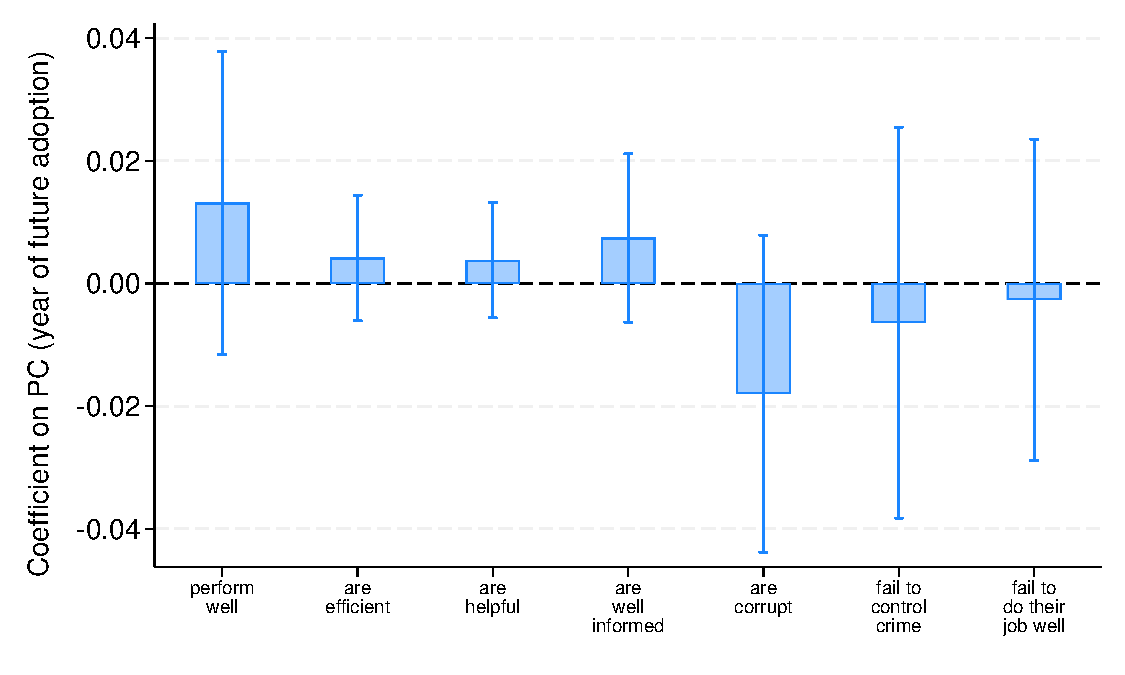
\includegraphics[width=\textwidth]{../manuscript/Graphs/balance_carabperc.pdf}
        \caption{Year of adoption and police performance before adoption}
    \end{subfigure}%
    ~
    \begin{subfigure}{0.495\textwidth}
        \centering
        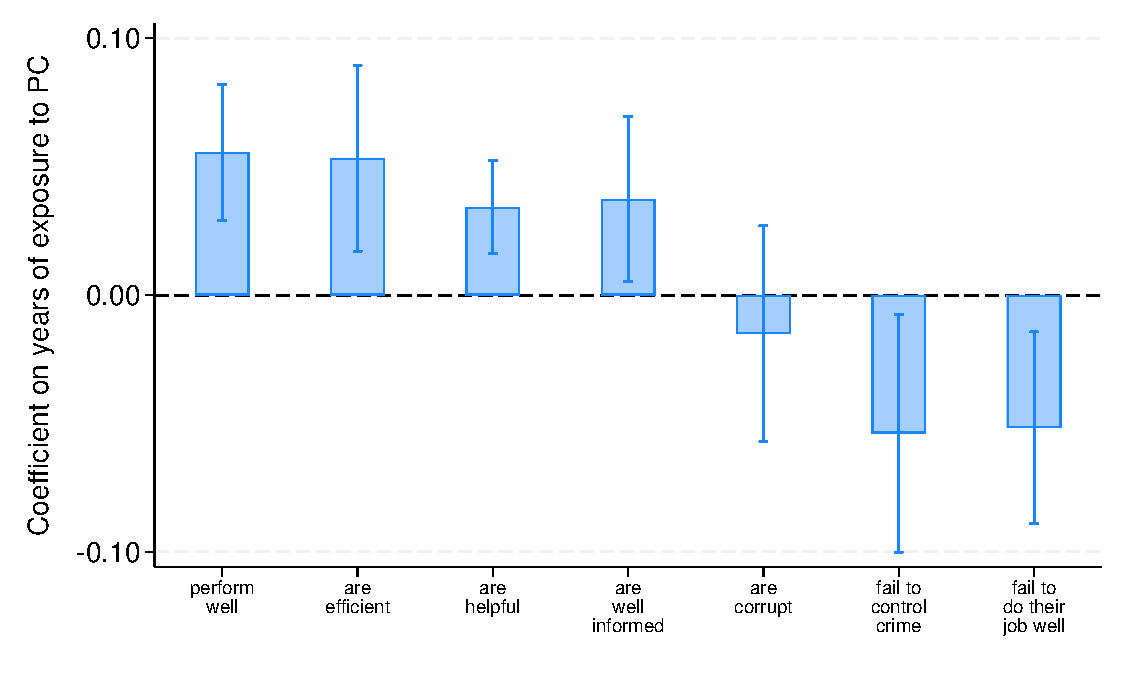
\includegraphics[width=\textwidth]{../manuscript/Graphs/doseresponse_carabperc.pdf}
        \caption{Years exposed to \emph{Plan Cuadrante} (dose response)}
    \end{subfigure}%
    \\[12pt]
    \begin{minipage}{0.99\textwidth}
    Notes: The figure considers seven measures of police performance: the share of respondents who perceive police performance as good, and who perceive the police to be efficient, helpful, well informed, corrupt, failing to control crime, and failing to do their job well. Using the sample of municipalities that adopted \emph{Plan Cuadrante} after 2005, panel (a) examines whether the future timing of adoption of \emph{Plan Cuadrante} is correlated with perceived police performance in 2005, before the introduction of the program. Panel (b) reestimates the same comparison as Figure \ref{fig:figure05}, replacing the binary adoption indicator with the municipality's number of years of exposure to \emph{Plan Cuadrante} as of 2005. In both panels, each bar plots the coefficient from a separate regression of one performance measure. The graphs display the estimated coefficients and 95\% confidence intervals.
    \end{minipage}
\end{figure}
}

\clearpage

{\renewcommand{\thefigure}{C.8}
\begin{figure}[h!]
    \centering
    \caption{Effects of \emph{Plan Cuadrante} on Reported Crime and Arrests Using the Full Set of Post-treatment and Pre-treatment Periods}
    \label{fig:admin_uncapped}
    \begin{subfigure}{0.495\textwidth}
        \centering
        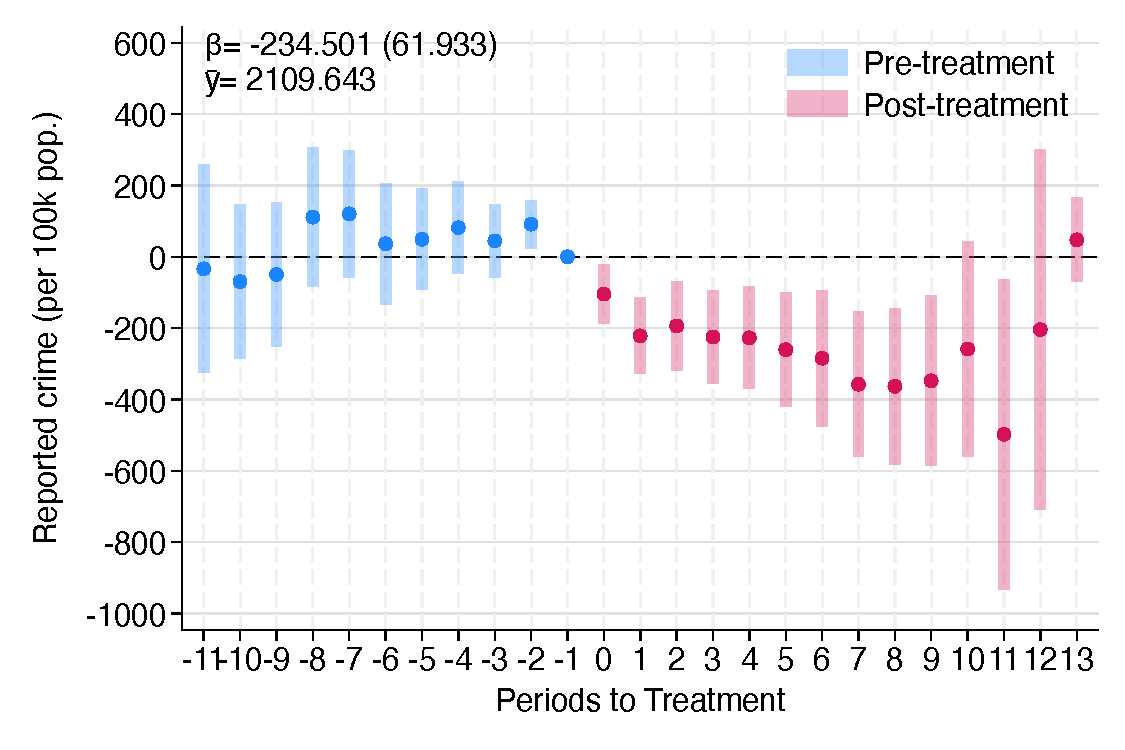
\includegraphics[width=0.98\textwidth]{../manuscript/Graphs/totalreportedcrime_allcomunas_uncapped.pdf}
        \caption{Reported crime per 100k inhabitants}
    \end{subfigure}%
    ~
    \begin{subfigure}{0.495\textwidth}
    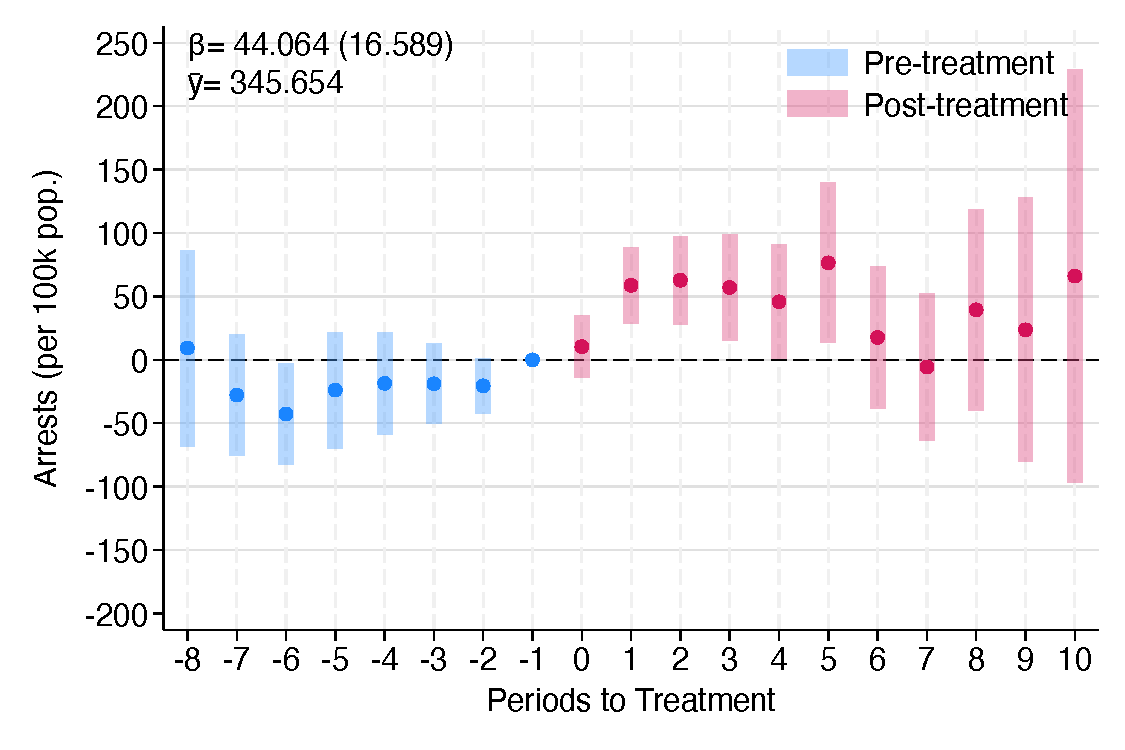
\includegraphics[width=0.98\textwidth]{../manuscript/Graphs/totalarrestscrime_allcomunas_uncapped.pdf}
        \caption{Arrests per 100k inhabitants}
    \end{subfigure}
    \begin{minipage}{\textwidth}
    \footnotesize
   Notes: This figure shows the dynamic effects of \emph{Plan Cuadrante} on the number of crimes reported to the police in the municipality per 100,000 inhabitants (panel a) and on the number of arrests in the municipality per 100,000 inhabitants (panel b), using administrative data. The estimation is conducted using the procedure developed in \citet{Callaway} for difference-in-differences with staggered treatment adoption. The dots in the figure represent the estimated coefficients and the bars behind them 95\% confidence intervals. Standard errors are clustered at the municipality level using the wild bootstrapping procedure. The pooled effect and the mean outcome before the introduction of the treatment are also presented in each panel. Unlike Figure \ref{fig:figure02} in the main text, we do not cap the event study to the same 5 pre-treatment and 6 post-treatment periods used for symmetry with the ENUSC-based analysis. Instead, we exploit the full set of post-treatment and pre-treatment periods. Panel (a) includes 4,371 observations and panel (b) 3,372 observations.
    \end{minipage}
\end{figure}
}

\clearpage

 
\end{response}
\stepcounter{AnsweredComments}

\begin{refcomment}
\smallskip

\textbf{Minor points:} 

1. Sample selection: I understand the final sample selection is driven by data availability, but sometimes I was confused by when the policy started and what years are covered by each data source. For example, survey data appear to be available from 2003, and administrative crime records also start in 2003 and run until 2018. Why, then, does the analysis stop in 2012? If this is due to survey availability, that should be made explicit, while the administrative data could still be shown descriptively for the later years. In addition, what distinguishes the municipalities included in the analysis from those excluded? How do early adopters compare to late adopters? For both the survey data and the police records, it would be useful to provide a comparison of characteristics between included and excluded municipalities to give readers confidence that the results are not being driven by sample selection.

\label{pt:r1_09}
\end{refcomment}

% Our reply to R1 - 9 
\begin{response}
	%Minor points

%Sample selection: I understand the final sample selection is driven by data availability, but sometimes I was confused by when the policy started and what years are covered by each data source. For example, survey data appear to be available from 2003, and administrative crime records also start in 2003 and run until 2018. Why, then, does the analysis stop in 2012? If this is due to survey availability, that should be made explicit, while the administrative data could still be shown descriptively for the later years. In addition, what distinguishes the municipalities included in the analysis from those excluded? How do early adopters compare to late adopters? For both the survey data and the police records, it would be useful to provide a comparison of characteristics between included and excluded municipalities to give readers confidence that the results are not being driven by sample selection.


Thank you very much for the opportunity to clarify this point. This is related to the availability of data by year and municipality across our two main data sources, and to how the \citet{Callaway} estimator is constructed. When the control group is formed from not-yet-treated units, the estimator only uses data up to the year in which the last treated unit in the data adopts the treatment.

Most outcomes in the paper rely on information from the ENUSC survey, which covers 101 urban municipalities. All of these municipalities were eventually treated except one. Because ENUSC was first conducted in 2003 and not administered in 2004, our main analytical sample includes the 46 urban municipalities that adopted \emph{Plan Cuadrante} between 2005 and 2012---the year in which the last municipality surveyed in ENUSC adopted the program---plus the one never-treated municipality. Even if the ENUSC survey were available after 2012, using these data in the estimation would mean relying only on this single never-treated municipality as the control group for all subsequent periods, which would make the estimates unreliable. We therefore limit the study period in the main analysis to 2003--2012.


Regarding the outcomes constructed from administrative records: these are provided by the Undersecretary for Crime Prevention and are available yearly for all Chilean municipalities---reported crimes from 2002 to 2016, and arrests from 2005 to 2016. This comprehensive coverage results in a much larger number of never-treated units, allowing for a longer estimation period that includes all the data period and municipalities adopting the program up to 2013, when the last Chilean municipality joined \emph{Plan Cuadrante}. In total, we use an analytical sample of 292 municipalities for reported crime and 281 for arrests. For simplicity and symmetry with the ENUSC-based analysis, our main specification nonetheless restricts the event study to 5 pre-treatment and 7 post-treatment periods. We show in Figure \ref{fig:admin_uncapped} in the updated manuscript that the results are very similar when the full set of pre- and post-adoption periods is used instead.

Below we reproduce the relevant paragraphs from the Data subsection of the updated manuscript:

\begin{adjustwidth}{2em}{0em}
We combine administrative and survey data from \emph{Carabineros}, the Undersecretary for Crime Prevention, and the National Institute of Statistics (INE).

\emph{Carabineros} provided information on \emph{Plan Cuadrante} implementation, which we use to define treatment status across municipalities over time. The National Institute of Statistics granted access to the National Survey on Security and Crime (ENUSC), a repeated cross-section first conducted in 2003 and administered annually between October and December since 2005. The survey covers more than 25,000 households across 101 urban municipalities, collecting information on crime victimization, perceptions, trust in police, and household prevention measures over the previous 12 months.\footnote{The survey is administered to a randomly selected household member who must: a) live in the household, b) be 15 years or older, c) not be a domestic worker, and d) not have any disability preventing survey comprehension.}

Our empirical approach excludes always-treated municipalities \citep{Callaway}. Given ENUSC's first implementation in 2003 and absence in 2004, our main sample includes households from 46 urban municipalities that adopted \emph{Plan Cuadrante} between 2005 and 2012 plus one never-treated municipality.\footnote{This sample excludes municipalities adopting \emph{Plan Cuadrante} in 2013 as they are not covered by ENUSC. Also, there is only one never treated municipality covered by ENUSC.} The treated municipalities in this analytical sample account for approximately 27\% of Chile's population.

The Undersecretary for Crime Prevention provided data on the number of reported crimes (2002--2016) and arrests (2005--2016) for all municipalities. This comprehensive coverage allows us to expand the analytical sample: for reported crime, we include all municipalities adopting \emph{Plan Cuadrante} after 2002 together with never-treated municipalities, for a total of 292 municipalities; for arrests, the corresponding sample includes all post-2005 adopters and never-treated municipalities, for a total of 281 municipalities. The treated municipalities in these analytical samples account for over half of Chile's population.

The study period differs across the two data sources, as each covers a different time span and a different set of municipalities. For the ENUSC-based analysis, it is restricted to 2003--2012. The \citet{Callaway} estimator uses not-yet-treated and never-treated municipalities as the comparison group. Since only one municipality in the survey sample is never treated, extending the analysis beyond 2012---the last year in which a municipality surveyed in ENUSC adopts the program---would leave only that single never-treated unit as the comparison group for subsequent periods, making the estimates unreliable. The administrative data, by contrast, cover a large number of never-treated municipalities that can serve as controls throughout the full data period, allowing us to exploit the complete administrative coverage---2002--2016 for reported crime and 2005--2016 for arrests---and to include all municipalities adopting the program from 2003 to 2013, when the last municipality joins \emph{Plan Cuadrante}.

Together, the treated municipalities in our two analytical samples represent substantial shares of the Chilean population---approximately 27\% in the ENUSC-based analysis and over half in the administrative data analysis---and are geographically distributed across the country rather than clustered in a single region. Tables \ref{tab:sum_statsA2} and \ref{tab:sum_statsA3} in Online Appendix \ref{sec:appendixA} and Table \ref{tab:comparing_samples} and Figure \ref{fig:pcsp_maps} in Online Appendix \ref{sec:appendixB} provide a detailed characterization of the treated municipalities in each analytical sample relative to the average Chilean municipality.
\end{adjustwidth}

Note the following footnote to Section 4 in the main manuscript:

\begin{adjustwidth}{2em}{0em}
Online Appendix Figure \ref{fig:admin_uncapped} reports the results for reported crime and arrests using the full set of post-treatment and pre-treatment periods, which are very similar to those presented here.
\end{adjustwidth}

and also the following subsection to Online Appendix C, ``Effects of \emph{Plan Cuadrante} Using the Full Set of Post-treatment and Pre-treatment Periods'':

\begin{adjustwidth}{2em}{0em}
For symmetry with the ENUSC-based analysis, the event studies for reported crime and arrests reported in the main text are restricted to 5 pre-treatment and 7 post-treatment periods. Because the administrative data are available for the full set of Chilean municipalities and therefore include a much larger number of never-treated municipalities than the ENUSC sample, we can estimate these effects over a longer window without exhausting the pool of valid comparison units. Figure \ref{fig:admin_uncapped} reports the effects of \emph{Plan Cuadrante} on reported crime and arrests using the full set of post-treatment and pre-treatment periods rather than capping the event study to the 5 pre-treatment and 7 post-treatment periods used in the main specification. The results are very similar to those presented in Section \ref{main_results}.
\end{adjustwidth}


Finally, we have added the following subsection, ``Characterization of the Analytical Samples,'' to Online Appendix B, comparing the characteristics of the municipalities included in each analytical sample with those excluded from it or always treated:

\begin{adjustwidth}{2em}{0em}
The treated municipalities in our analytical samples are geographically distributed across the country. As shown in Figure \ref{fig:pcsp_maps}, the 46 treated municipalities in the ENUSC-based sample span Chile from north to south, covering a wide range of geographic and socioeconomic contexts, and together account for approximately 27\% of Chile's population. The 96 treated municipalities in the administrative data sample provide even broader national coverage, together accounting for over half of Chile's population.

Table \ref{tab:comparing_samples} characterizes the treated municipalities in each analytical sample relative to all Chilean municipalities (Column 1), all \emph{Plan Cuadrante} municipalities (Column 2), the always-treated municipalities excluded from our estimation samples (Column 3), and never-treated municipalities (Column 6). Columns (4) and (5) report characteristics for the treated municipalities in the ENUSC and administrative data analytical samples respectively. On several dimensions our samples broadly resemble the overall Chilean population: the poverty rate of the 46 treated municipalities in the ENUSC sample (21.7\%) and the 96 treated municipalities in the administrative data sample (24.0\%) are both close to the national average of 23.7\%, and the crime rates of the treated ENUSC municipalities closely track the average across all \emph{Plan Cuadrante} municipalities (2,202 vs.\ 2,132 per 100,000 inhabitants). They do differ on other dimensions---particularly crime rates relative to all Chilean municipalities and population density---but both differences have natural explanations. Higher crime rates are expected because \emph{Plan Cuadrante} exclusively targeted urban municipalities, where crime is more prevalent. The lower-than-average population density in our samples (215 and 135 inhabitants per km$^2$, vs.\ a national mean of 870) reflects the fact that the most densely populated \emph{Plan Cuadrante} municipalities---those of the Santiago metropolitan area---were the earliest adopters of the program and are therefore excluded from our analytical samples as always-treated.
\end{adjustwidth}





\clearpage
\noindent\textbf{Other figures and tables referenced above:}
\vspace{0.5em}

{\renewcommand{\thefigure}{C.8}
\begin{figure}[h!]
    \centering
    \caption{Effects of \emph{Plan Cuadrante} on Reported Crime and Arrests Using the Full Set of Post-treatment and Pre-treatment Periods}
    \label{fig:admin_uncapped}
    \begin{subfigure}{0.495\textwidth}
        \centering
        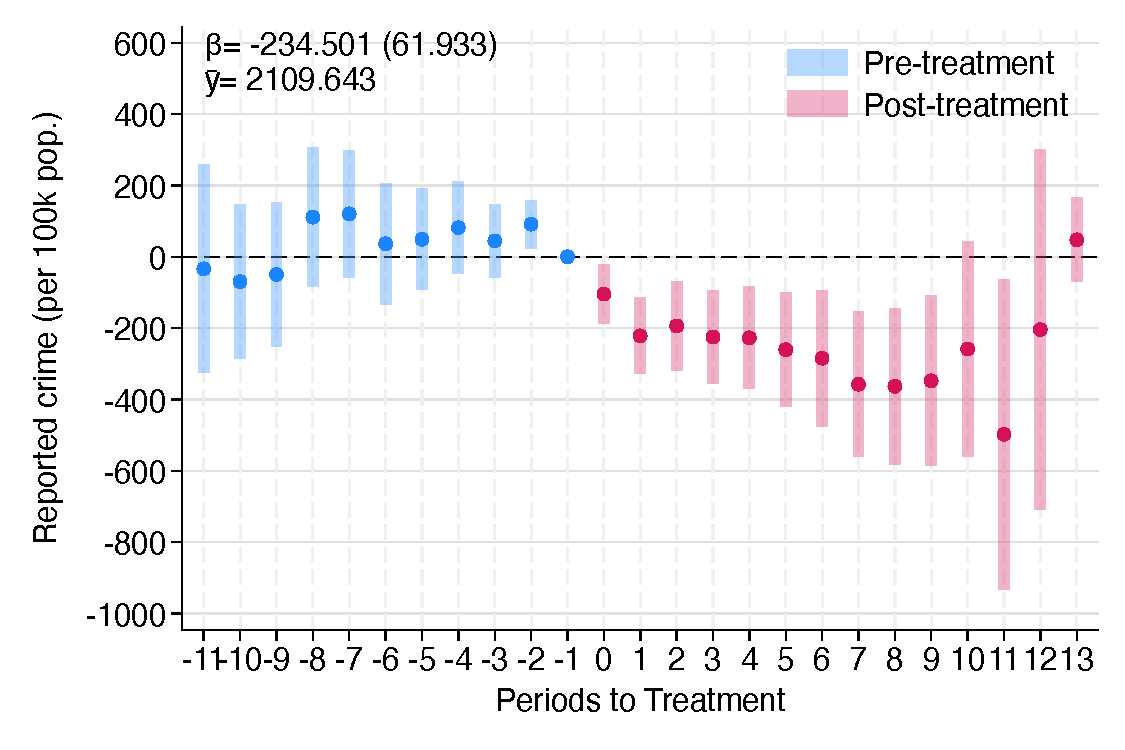
\includegraphics[width=0.98\textwidth]{../manuscript/Graphs/totalreportedcrime_allcomunas_uncapped.pdf}
        \caption{Reported crime per 100k inhabitants}
    \end{subfigure}%
    ~
    \begin{subfigure}{0.495\textwidth}
    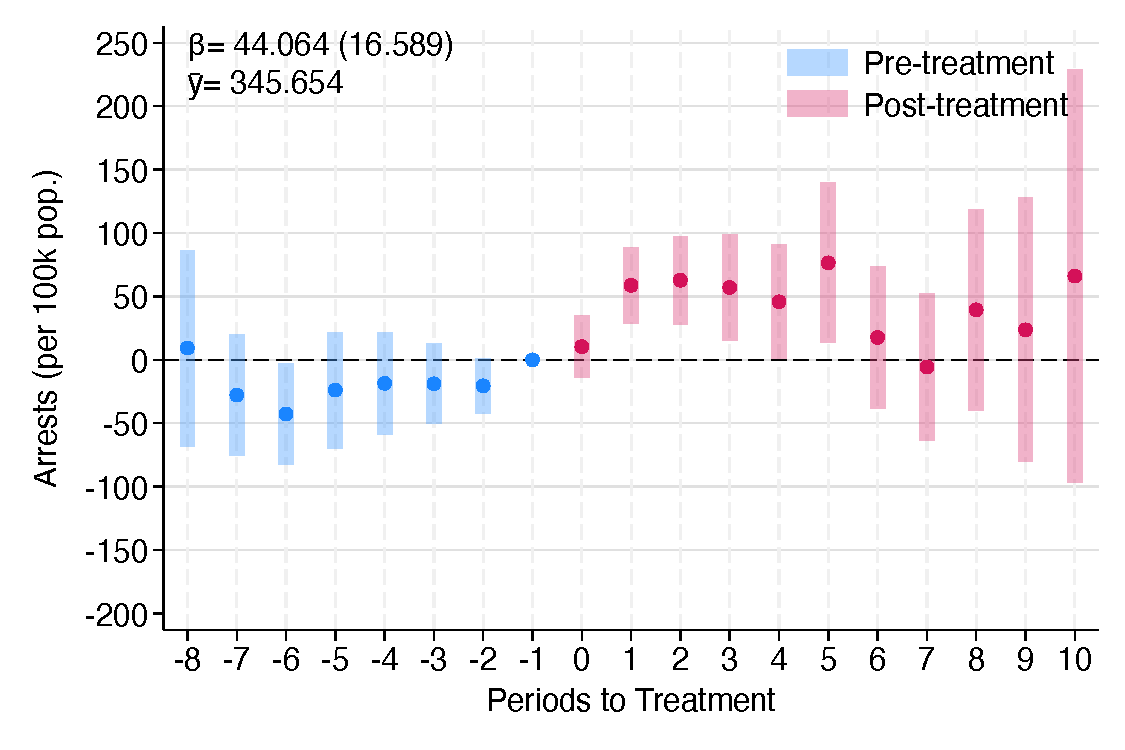
\includegraphics[width=0.98\textwidth]{../manuscript/Graphs/totalarrestscrime_allcomunas_uncapped.pdf}
        \caption{Arrests per 100k inhabitants}
    \end{subfigure}
    \begin{minipage}{\textwidth}
    \footnotesize
   Notes: This figure shows the dynamic effects of \emph{Plan Cuadrante} on the number of crimes reported to the police in the municipality per 100,000 inhabitants (panel a) and on the number of arrests in the municipality per 100,000 inhabitants (panel b), using administrative data. The estimation is conducted using the procedure developed in \citet{Callaway} for difference-in-differences with staggered treatment adoption. The dots in the figure represent the estimated coefficients and the bars behind them 95\% confidence intervals. Standard errors are clustered at the municipality level using the wild bootstrapping procedure. The pooled effect and the mean outcome before the introduction of the treatment are also presented in each panel. Unlike Figure \ref{fig:figure02} in the main text, we do not cap the event study to the same 5 pre-treatment and 6 post-treatment periods used for symmetry with the ENUSC-based analysis. Instead, we exploit the full set of post-treatment and pre-treatment periods. Panel (a) includes 4,371 observations and panel (b) 3,372 observations.
    \end{minipage}
\end{figure}
}

\clearpage

{\renewcommand{\thetable}{A.2}
\begin{table}[H]
\centering
\caption{Summary Statistics -- ENUSC sample}
\label{tab:sum_statsA2}
\begin{threeparttable}
\begin{tabular}{l r r r r r}
\toprule
 & Mean & SD & Min & Max & N \\
\midrule
\multicolumn{6}{@{}l}{\textit{Household}} \\
\quad Socioeconomic status               & 3.58  & 0.73  & 1    & 5    & 99,298 \\
\quad Victimization                    & 0.26  & 0.44  & 0    & 1    & 99,298 \\
\quad Crime perception (neighborhood)  & 0.38  & 0.49  & 0    & 1    & 95,598 \\
\quad Crime perception (municipality)  & 0.66  & 0.48  & 0    & 1    & 96,794 \\
\quad Crime perception (country)       & 0.79  & 0.41  & 0    & 1    & 98,525 \\
\quad Trust in the police              & 0.44  & 0.50  & 0    & 1    & 51,445 \\
\quad Investment in security measures  & 0.21  & 0.40  & 0    & 1    & 99,298 \\
\quad \emph{Plan Cuadrante} (year)                  & 2007  & 1.85  & 2005 & 2012 & 97,847 \\
\addlinespace
\multicolumn{6}{@{}l}{\textit{Household member interviewed}} \\
\quad Female                      & 0.55  & 0.50  & 0  & 1  & 99,298 \\
\quad Age                         & 43.87 & 17.95 & 15 & 99 & 99,298 \\
\quad Primary school attendance   & 0.98  & 0.14  & 0  & 1  & 99,298 \\
\quad Secondary school attendance & 0.72  & 0.45  & 0  & 1  & 99,298 \\
\quad University attendance       & 0.20  & 0.40  & 0  & 1  & 99,298 \\
\bottomrule
\end{tabular}
\begin{tablenotes}[flushleft]
\footnotesize
\item Note: This table presents summary statistics from the ENUSC sample, covering the 47 municipalities used in the survey-based analysis (46 that adopted \emph{Plan Cuadrante} between 2005 and 2012 plus one never-treated municipality). Socioeconomic status is a 1 to 5 measure produced by ENUSC surveys and based on self-reported socioeconomic strata, being 1 the highest ranked and 5 the lowest. Crime perception is equal to 1 if the interviewed person reports that crime has increased in the last 12 months. The \emph{Plan Cuadrante} (year) row is computed over treated municipalities only.
\end{tablenotes}
\end{threeparttable}
\end{table}
}

\clearpage

{\renewcommand{\thetable}{A.3}
\begin{table}[H]
\centering
\caption{Summary Statistics -- Administrative municipality level sample}
\label{tab:sum_statsA3}
\begin{threeparttable}
\begin{tabular}{l r r r r r}
\toprule
 & Mean & SD & Min & Max & N \\
\midrule
\multicolumn{6}{@{}l}{\textit{Panel A. Reported-crime sample (292 municipalities)}} \\
\quad Reported crime (per 100k pop.)            & 1,732.39 & 1,036.68 & 0.00   & 11,434.40 & 4,371 \\
\quad Arrests (per 100k pop.)                   & 332.07   & 271.75   & 0.00   & 1,712.30  & 3,504 \\
\quad Poverty rate (\%)                         & 25.74    & 9.72     & 5.65   & 58.33     & 3,720 \\
\quad Pop.\ density (pop./km\textsuperscript{2}) & 63.51   & 140.47   & 0.09   & 1,109.58  & 4,065 \\
\quad \emph{Plan Cuadrante} (year)                     & 2010     & 2.82     & 2003   & 2013      & 1,440 \\
\addlinespace
\multicolumn{6}{@{}l}{\textit{Panel B. Arrests sample (281 municipalities)}} \\
\quad Reported crime (per 100k pop.)            & 1,684.74 & 1,014.67 & 0.00   & 11,434.40 & 4,209 \\
\quad Arrests (per 100k pop.)                   & 313.21   & 251.23   & 0.00   & 1,712.30  & 3,372 \\
\quad Poverty rate (\%)                         & 26.01    & 9.72     & 5.65   & 58.33     & 3,570 \\
\quad Pop.\ density (pop./km\textsuperscript{2}) & 57.90   & 127.30   & 0.09   & 1,109.58  & 3,900 \\
\quad \emph{Plan Cuadrante} (year)                     & 2010     & 2.26     & 2006   & 2013      & 1,275 \\
\bottomrule
\end{tabular}
\begin{tablenotes}[flushleft]
\footnotesize
\item Note: The table reports municipality-level summary statistics for the two administrative estimation samples used in the paper. Panel A covers the 292 municipalities in the reported-crime sample (municipalities adopting \emph{Plan Cuadrante} from 2003 onward plus never-treated); Panel B the 281 municipalities in the arrests sample (adopters from 2006 onward plus never-treated --- municipalities adopting in 2005 are excluded because arrest data begin that year, leaving no pre-treatment period). Reported crime and arrests are measured per 100,000 inhabitants over 2002--2016 and 2005--2016, respectively. Minimum reported crime and arrests of zero correspond to tiny, remote never-treated comunas (e.g., Juan Fernández, Cabo de Hornos). The \emph{Plan Cuadrante} (year) row is computed over treated municipalities only. Data from the Undersecretary for Crime Prevention.
\end{tablenotes}
\end{threeparttable}
\end{table}
}

\clearpage

{\renewcommand{\thefigure}{B.1}
\begin{figure}[h!]
    \centering
    \caption{Geographic Distribution of \emph{Plan Cuadrante}}
    \label{fig:pcsp_maps}
    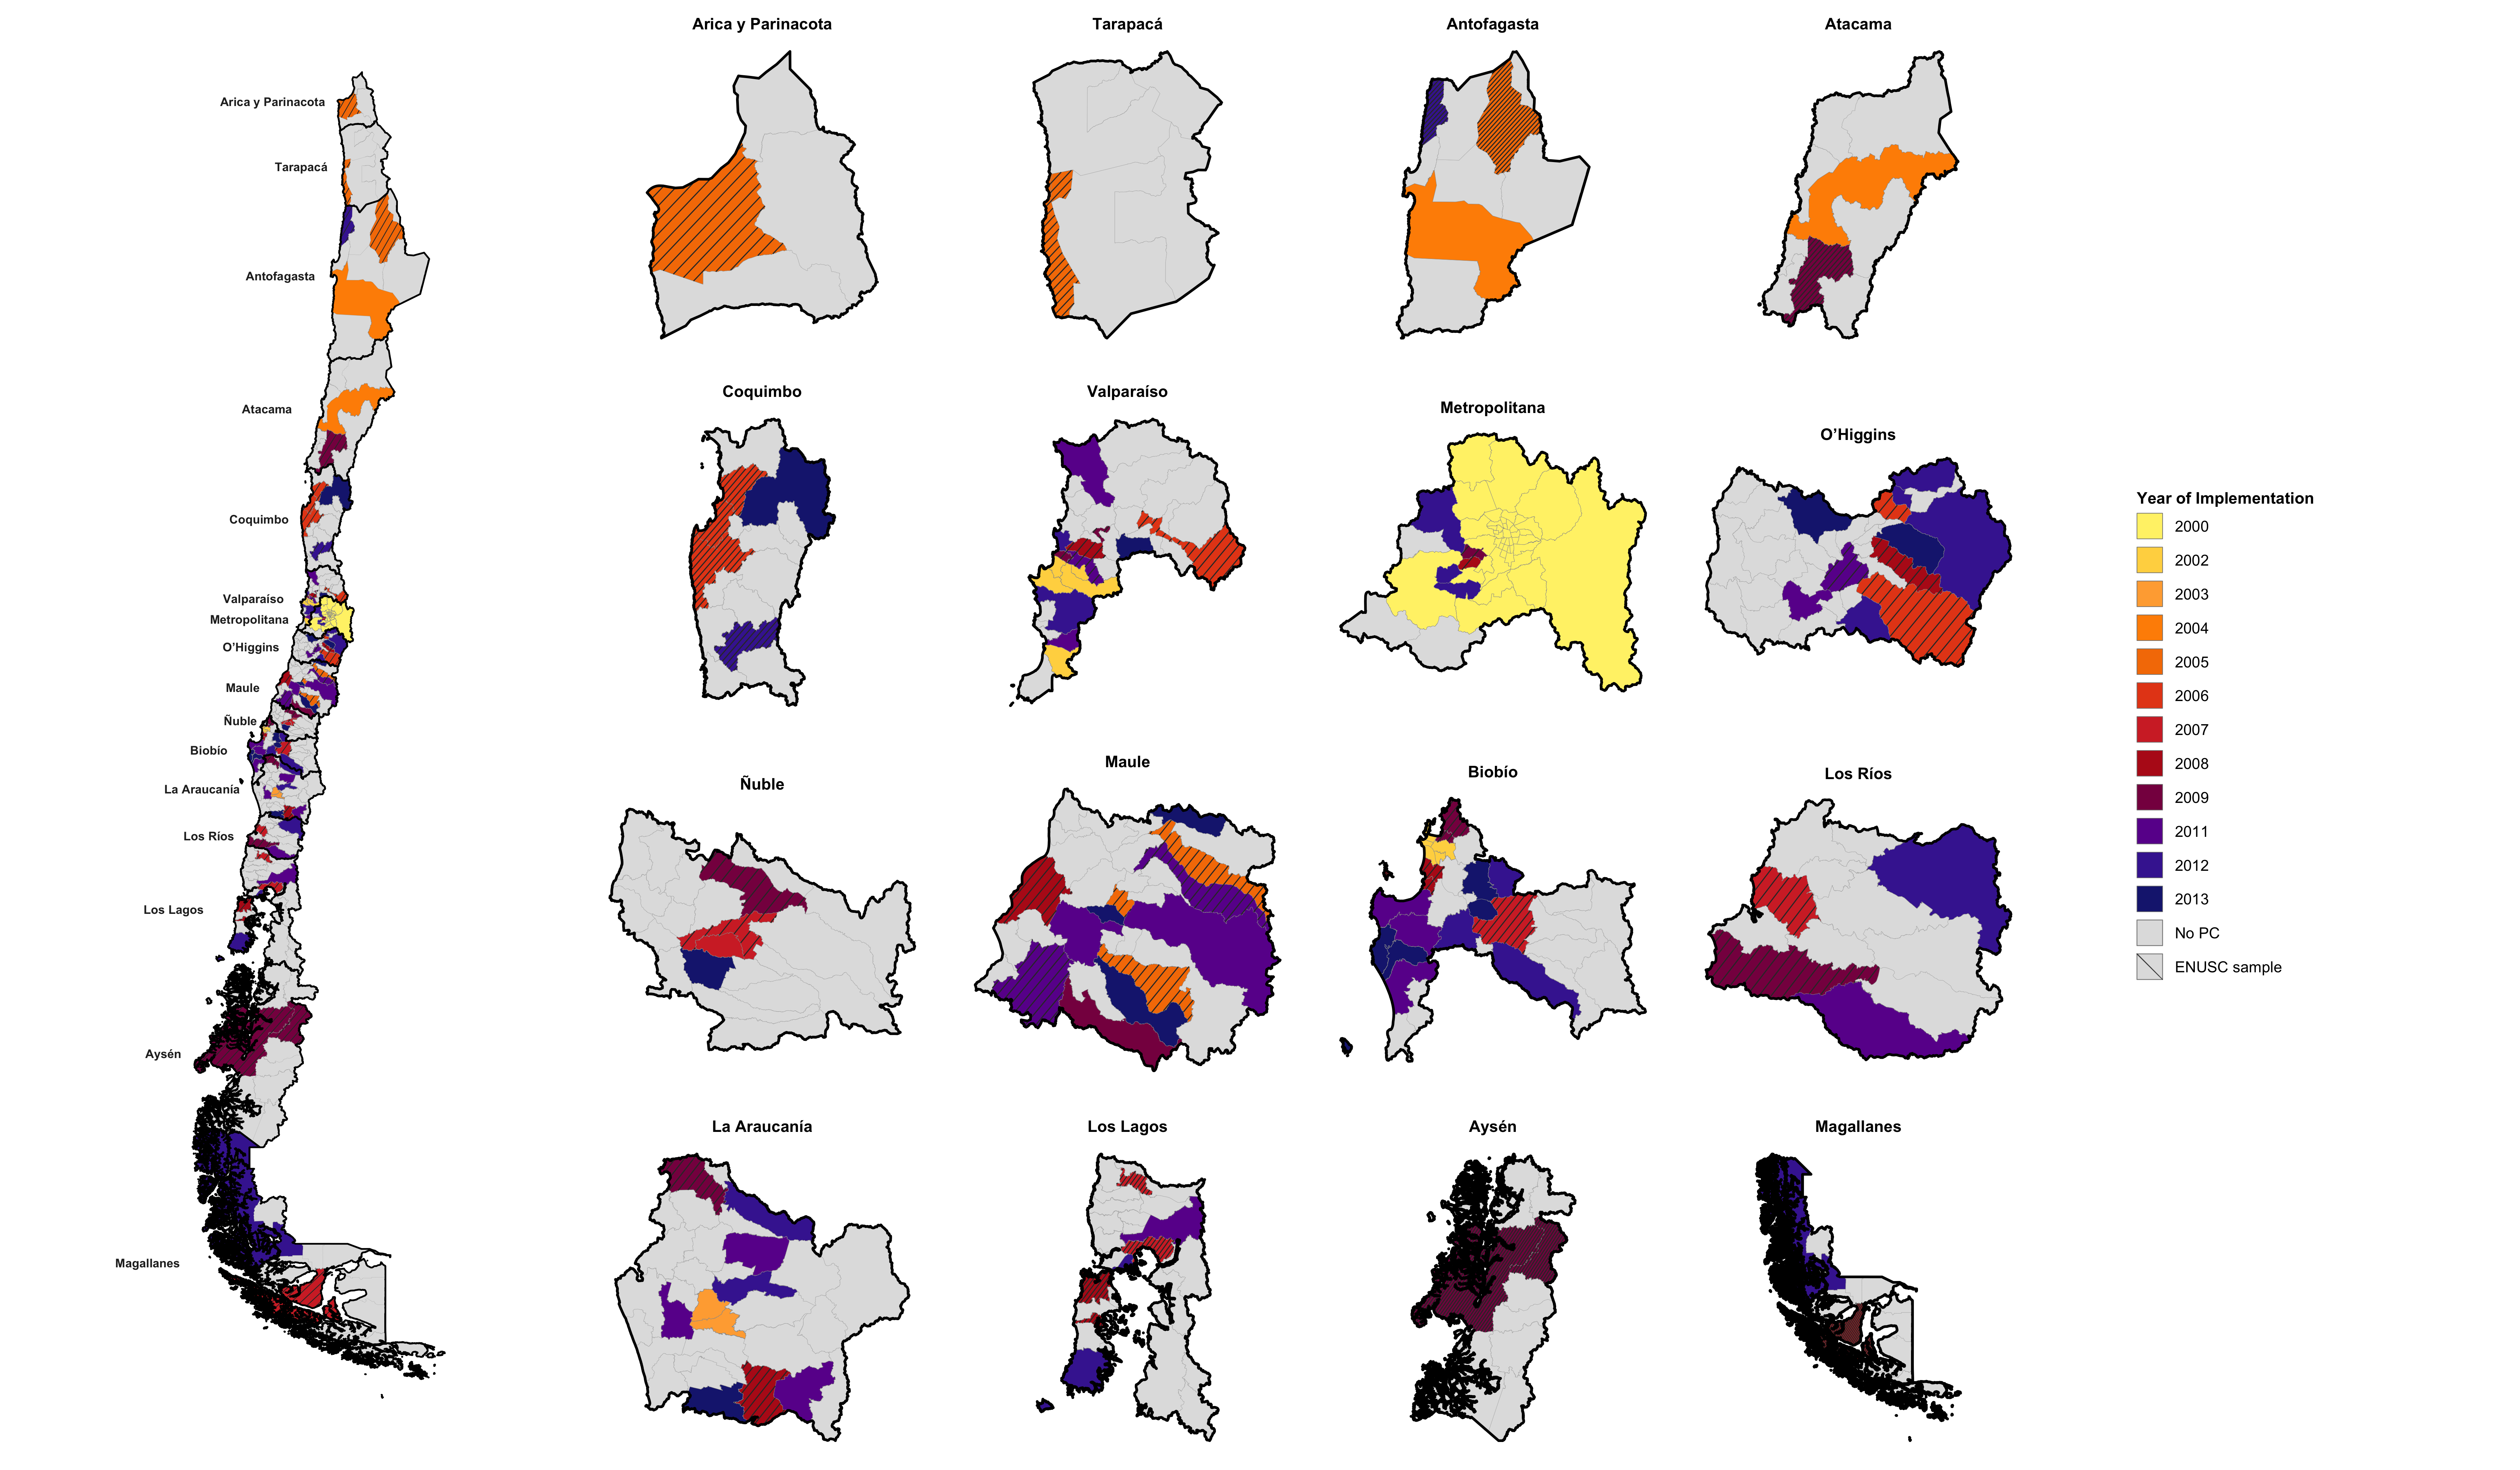
\includegraphics[width=\textwidth]{../manuscript/Graphs/mapa_PCSP_Chile_combinado.png}
    \begin{minipage}{0.95\textwidth}
    \footnotesize
    Notes: This figure shows the spatial rollout of \emph{Plan Cuadrante} across Chilean municipalities. The national map (left) is displayed alongside the 16 regional maps (right) for closer inspection. The color of each treated municipality indicates its year of program adoption, ranging from 2000 (lightest) to 2013 (darkest), following the legend. Municipalities shown in light grey were never treated under PC. Diagonal hatching identifies the 46 treated municipalities in the analytical sample used to estimate the effects on ENUSC outcomes.
    \end{minipage}
\end{figure}
}

\clearpage

{\renewcommand{\thetable}{B.1}
\begin{table}[H]
\caption{Baseline characteristics by subsample}
\label{tab:comparing_samples}
\begin{center}
\resizebox{\textwidth}{!}{
\begin{threeparttable}
\begin{tabular}{l cccccc}
\toprule
&  & \multicolumn{4}{c}{PC municipalities}  & \\
\cmidrule(lr){3-6}
& (1) & (2) & (3) & (4) & (5) & (6) \\
& All & All PC & Always- & Treated & Treated & Never- \\
& municipalities & municipalities & treated & ENUSC & admin.\ data & treated \\
\midrule
Reported crime (per 100k pop.) &     1,650.23 &     2,132.29 &     2,437.25 &     2,202.06 &     1,976.59 &     1,282.47 \\
Arrests (per 100k pop.)        &       267.62     &       442.08     &       606.01     &       459.05     &       358.11     &       134.11     \\
Poverty rate (\%)              &        23.73     &        20.50     &        14.88     &        21.73     &        23.96     &        26.82     \\
Pop.\ density (pop./km$^2$)   &       870.28 &     1,904.14 &     4,593.32 &       215.52 &       134.50 &        27.02 \\
Population                     &    57,857.22         &   117,975.43         &   187,558.74         &   113,079.74         &    81,532.84         &    11,612.44         \\
\midrule
Municipalities                 &          346            &          150            &           58            &           46            &           96            &          196            \\
\bottomrule
\end{tabular}
\begin{tablenotes}[flushleft]
\footnotesize{\item Note: Reported crime, poverty rate, population density, and population are measured as of 2003; arrests are measured as of 2005, the first year for which arrest data are available. Column (1) includes all municipalities in Chile. Column (2) includes all PC municipalities. Column (3) restricts to municipalities that adopted \emph{Plan Cuadrante} before 2005, the always-treated in our sample, which are therefore excluded from our estimation samples (as depicted in Figure 1, panel (a)). Column (4) restricts to treated municipalities in the analytical sample using the ENUSC data. Column (5) restricts to treated municipalities included in the analytical sample using the administrative data. Column (6) includes never-treated municipalities.}
\end{tablenotes}
\end{threeparttable}}
\end{center}
\end{table}
}

\clearpage
 
\end{response}
\stepcounter{AnsweredComments}

\begin{refcomment}
\smallskip

2. Online Appendix C has the wrong reference on page 4.

\label{pt:r1_10}
\end{refcomment}

% Our reply to R1 - 10 
\begin{response}
	%Online Appendix C has the wrong reference on page 4.

Thanks for spotting the mistake. We replaced with the correct reference in the updated manuscript. 
\end{response}
\stepcounter{AnsweredComments}

\putbib
\end{bibunit}

%-----------------------------------------------------------------------------------------




